\documentclass[a4paper,11pt,spanish]{book}
%\usepackage[utf8]{inputenc}
\usepackage[utf8x]{inputenc}
\usepackage{url}
\usepackage{makeidx}
\usepackage[procnames]{listings}
\usepackage{color}
\usepackage{graphicx} % graficos
\usepackage{subfig}
\usepackage{tabularx}
%\usepackage{subcaption}
\captionsetup{compatibility=false}
\usepackage[export]{adjustbox}
\usepackage[spanish]{babel}
\usepackage{mathtools}
\usepackage[chapter]{algorithm}
\usepackage{algorithmicx}
\usepackage{algpseudocode}
%\usepackage[options]{natbib}
\usepackage{verbatim, amsmath, amsfonts, amssymb, amsthm} % For code environment and math support

\usepackage{fullpage}


\newcommand*{\FIXME}[1]{{(\textbf{FIXME}) {#1}}}

\iffalse
\let\mylistof\listof
\renewcommand\listof[2]{%
  \mylistof{algorithm}{Lista de Algortimos}%
}
\fi

\iffalse
\title{Transferencia de Estilo en Fotografias utilizando Redes Neuronales Convolucionales}   %note \\[1ex] is a line break in the title

\author{Wolfmann, Ariel Mauricio}             %your name
\college{Facultad de Matemática, Astronomía y Física\\[1ex]
		}  %your college
\university{Universidad Nacional de Córdoba}

%\renewcommand{\submittedtext}{change the default text here if needed}
%\degree{Licenciada en Ciencias de la Computación}     %the degree
\directors{Sanchez, Jorge}
\fi

\makeindex



\begin{document}
\definecolor{keywords}{RGB}{255,0,90}
\definecolor{comments}{RGB}{0,0,113}
\definecolor{red}{RGB}{160,0,0}
\definecolor{green}{RGB}{0,150,0}

\lstset{language=Python,
        basicstyle=\ttfamily\small,
        keywordstyle=\color{keywords},
        commentstyle=\color{comments},
        stringstyle=\color{red},
        showstringspaces=false,
        identifierstyle=\color{green},
        procnamekeys={def,class}}


\begin{titlepage}
  \begin{center}
  \vspace*{1in}
    \begin{Huge}
    \textbf{Trabajo Final}\\
    \textbf{Transferencia de Estilo en Fotografias utilizando Redes Neuronales Convolucionales} \\
    \end{Huge}
  \end{center}
  \begin{center}
    \begin{large}
      \vspace*{1in}
      Autor: Wolfmann, Ariel Mauricio\\
      Director: Sanchez, Jorge\\
    \end{large}
    \vspace*{0.15in}
     Marzo de 2017\\
    \vspace*{0.15in}
    Universidad Nacional de Córdoba\\
    \vspace*{0.15in}
    Facultad de Matemática, Astronomía y Física\\
    \vspace*{0.6in}
  \end{center}
\end{titlepage}

\iffalse
\maketitle                  % create a title page from the preamble info
\include{abstract}          % include the abstract
\include{dedication}        % include a dedication.tex file
\include{acknowlegements}   % include an acknowledgements.tex file

\begin{romanpages}          % start roman page numbering
\tableofcontents            % generate and include a table of contents
\listoffigures              % generate and include a list of figures
\end{romanpages}            % end roman page numbering
\fi

\tableofcontents
%\listoffigures
%\listofalgorithms

\chapter{Introducción}
  \section {Contexto}
    En los últimos años las fotografías están pasando a ser un objeto digital en lugar de físico, de la mano del gran aumento en el uso de los dispositivos móviles.
    Cualquier persona puede tomar miles de fotografías en un instante de tiempo, y compartirlas en las redes sociales, desde su propio dispositivo.
    A partir de esto, se han desarrollado muchas aplicaciones entorno a las fotografías ya sea, desde redes sociales masivamente utilizadas hasta aplicaciones que aplican efectos
    o filtros a la fotografía para transformarla en un retrato en blanco y negro o sepia por ejemplo.

    Muy recientemente se han comenzado a desarrollar aplicaciones que logran transferir el estilo de una obra de arte a una fotografía. Esto es posible gracias al incremento
    del poder de cómputo y al descenso del precio de los nuevos dispositivos, ya que las técnicas computacionales empleadas para lograr esto, requieren un cómputo mucho mas complejo
    y demandante.

    La transferencia de estilo requiere de la interacción de 2 de las principales áreas de las Ciencias de la Computación, de gran auge en la actualidad: Visión por Computadoras y Aprendizaje Automático,
    mas específicamente Aprendizaje Profundo.
    Hasta hace un tiempo estas areas fueron evolucionando en paralelo, independientemente una de la otra. Hoy en día se han logrado resultados completamente disruptivos, al aplicar
    Aprendizaje Profundo para algunas de las principales tareas de Visión por Computadoras, como lo son la clasificación de imágenes, detección y reconocimiento de objetos.

    \paragraph{Aprendizaje Automático}
      El área de Aprendizaje Automático es el área de las Ciencias de la Computación que explora el estudio y la construcción de algoritmos que pueden aprender y hacer predicciones
      sobre los datos de entrada.
      Tales algoritmos logran aprender a inferir caracteristicas que poseen los datos, a traves de la construcción de un modelo de predicción, en la etapa de entrenamiento del modelo.
      Cuando finaliza esta etapa, el modelo debe ser capaz de predecir caracteristicas de una muestra nueva, nunca antes vista, en base a lo aprendido en el entrenamiento.

      El principal objetivo de un sistema de aprendizaje es generalizar desde su experiencia o conocimiento previo. Generalizar en este contexto es la habilidad del sistema de realizar
      predicciones con precisión sobre un ejemplo nuevo no visto antes, luego de aprender sobre el conjunto de entrenamiento. Estos ejemplos de entrenamiento provienen de un espacio
      con probabilidad de distribución desconocida del cual es considerado representativo. El sistema de aprendizaje debe construir un modelo o función sobre el espacio total que le permita realizar
      predicciones lo suficientemente precisas sobre nuevos ejemplos. El modelo aprende una función de predicción $F$, a partir del conjunto de instancias de entrenamiento,
      cada una de ellas, representada por un vector de características.  Durante el entrenamiento, $F$  \emph{aprende a predecir}, ajustandose a estos vectores.
      Segun Mitchell, considerado uno de los impulsores del uso masivo del aprendizaje automático, “Un modelo que aprende no asume nada acerca de la identidad del concepto objetivo,
      no tiene ninguna base racional para clasificar cosas que nunca vio” \cite{Mitchell:1997:ML:541177}.

      El aprendizaje automático esta ideado para ser empleado en una serie de tareas informáticas en las que el diseño y la programación de algoritmos explícitos son inviables,
      como por ejemplo para la detección de Spam, el reconocimiento óptico de caracteres y los motores de búsqueda \cite{Bishop:MachineLearning}.

      Dentro del Aprendizaje Automático, existe un subdominio llamado Aprendizaje Profundo, que ataca problemas complejos en los cuales representar una instancia no es una tarea sencilla.
      Por ejemplo para representar una imagen se suelen utilizar sus pixeles o pequeñas subregiones de pixeles, sin embargo estas representacion no logran capturar caracteristicas de
      alto nivel, como es el caso de detectar si existe o no un ojo dada una subregion de pixeles de la imagen.

      Dado a que en este tipo de problemas no hay representacion intuitiva clara de los datos, los algoritmos de aprendizaje automático aprenden no solo a realizar predicciones, sino
      que tambien aprenden a representar los datos de entrada, capturando caracteristicas de alto nivel, de forma tal que la predicción en base a estas representaciones sea lo mas precisa posible \cite{Goodfellow-et-al-2016}.

      Para el caso de los problemas relacionados con imagenes, la tecnica de aprendizaje profundo mayormente utilizada es la de Redes Neuronales Convolucionales.
      Estas redes, son un tipo especifico de Redes Neuronales Artificiales, que asumen explicitamente que los datos de entrada seran imagenes, lo cual permite implementar
      ciertas optimizaciones dentro del algoritmo. Todos estos conceptos seran posteriormente explicados en detalle a lo largo del siguiente capítulo.

      Un ejemplo de amplia investigación y desarrollo en la actualidad, es el de los vehiculos autonomos,
      los cuales emplean estas técnicas de aprendizaje profundo dentro de sus procesos para la detección de objetos en tiempo real, como se puede observar en la figura \ref{fig:car_detection}.

      \begin{figure}[h]
	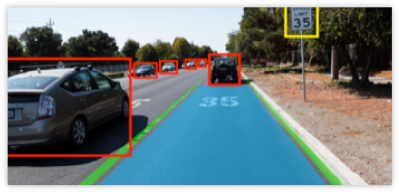
\includegraphics[width=0.9\linewidth]{./img/nvidia_car_detection.png}
	\caption{Vehiculo conducido automaticamente, detectando objetos en tiempo real mediante Redes Neuronales Convolucionales}
	\label{fig:car_detection}
      \end{figure}

    \paragraph{Visión por Computadoras}
      El área de Visión por Computadoras es el área de las Ciencias de la Computación encargado de lograr que las computadoras pueden lograr obtener una comprensión de alto nivel de imágenes digitales o vídeos.
      Desde la perspectiva de la ingeniería, busca automatizar tareas que el sistema visual humano puede hacer. Para lograr este nivel de comprensión, en primer lugar emplea métodos de bajo nivel relacionados
      con el Procesamiento de Imagenes para adquirir, procesar, analizar y comprender las imágenes del mundo real con el fin de producir información numérica o simbólica para que
      puedan ser tratados por una computadora. Generalmente la salida de estos metodos suele ser una imagen preprocesada o un conjunto de parametros calculados que sirven como entrada
      para que los metodos de Visión por Computadoras obtengan información de alto nivel a partir de estos.
      El objetivo principal de esta area es reducir la distancia
      entre lo que un humano interpreta a partir de una imagen y la forma en la que las computadoras representan esa misma imagen \cite{Szeliski:ComputerVision}.

      La transferencia de estilo en fotografías es considerado un problema complejo dentro del area de vision por computadoras, por lo que, luego de realizar diferentes investigaciones se
      decidio atacarlo utilizando las Redes Neuronales Convolucionales, como lo hace Gatys et. al \cite{Gatys:Neural_Style}.
      Para introducir al lector en el tema en la figura \ref{fig:style_transfer_candy_tower} se puede observar un ejemplo del resultado de aplicar la transferencia de estilo en fotografias:
      Como imagen de estilo se eligio una imagen abstracta \ref{fig:candy} y como imagen de contenido una fotografia de un paisaje \ref{fig:tower}, obteniendo como resultado de la
      transferencia de estilo una imagen en la cual se mantienen las estructuras de la imagen de contenido pero con los colores y trazos de la imagen de estilo \ref{fig:candy_tower}
      \begin{figure}[h]
	\subfloat[Imagen de Estilo]{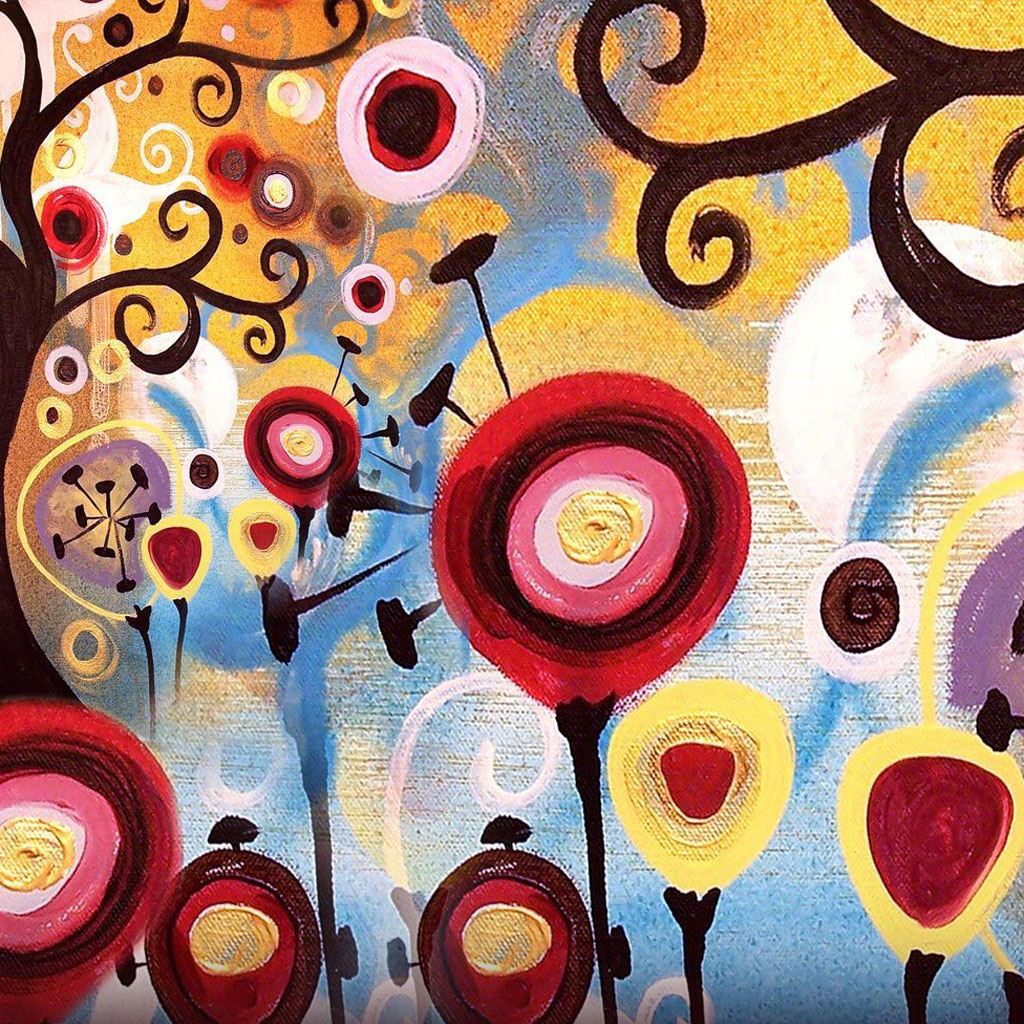
\includegraphics[height=0.27\textheight]{./img/jhonson_style_candy.jpg}\label{fig:candy}}
	\subfloat[Imagen de Contenido]{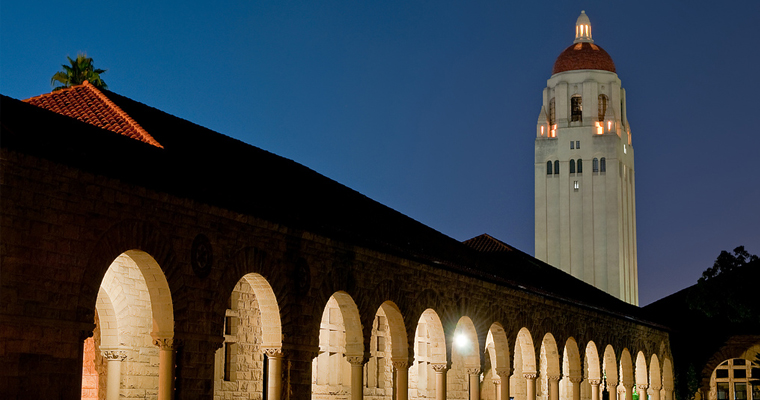
\includegraphics[height=0.27\textheight]{./img/jhonson_content_tower.jpg}\label{fig:tower}}
	\subfloat[Resultado obtenido transfiriendo el estilo de la obra de arte a la imagen de contenido]
	{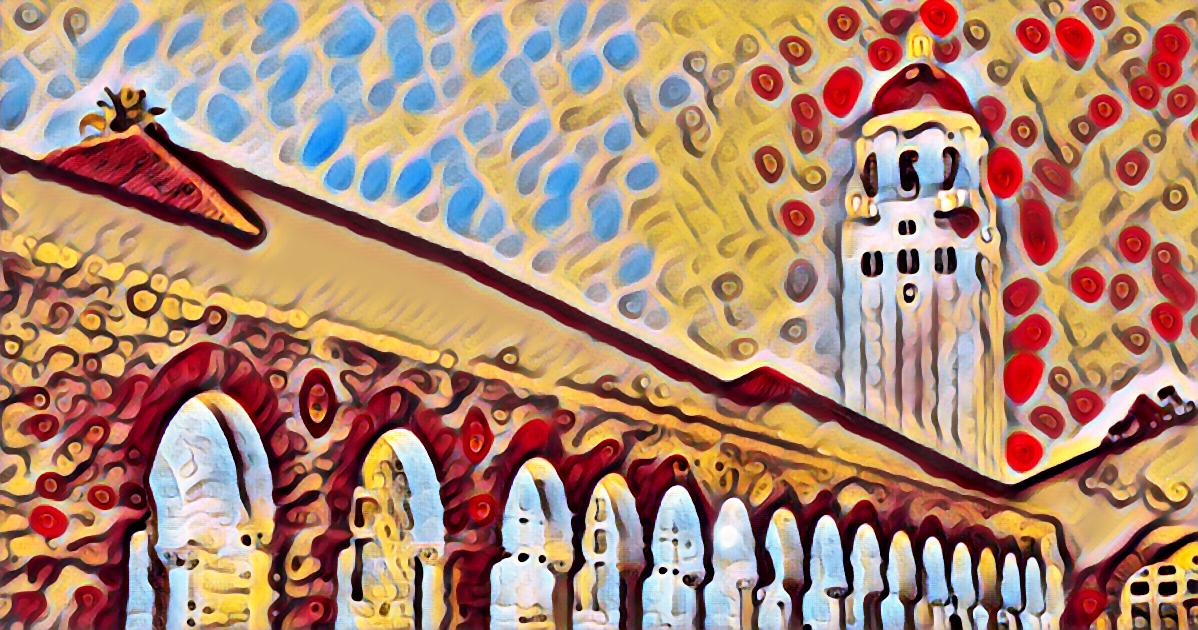
\includegraphics[height=0.27\textheight]{./img/jhonson_result_tower_candy.jpg}\label{fig:candy_tower}}
	\caption{Ejemplo de transferencia de estilo}
	\label{fig:style_transfer_candy_tower}
      \end{figure}
  \section {Motivación}
    Una imagen, digitalmente, es representada por un arreglo de 2 dimensiones donde cada valor representa la intensidad captada por un sensor
    de un determinado punto espacial, representados como píxeles. La representación de los píxeles es muy sensible a cambios en la iluminación, ángulo, contraste y tamaño que pueda existir.

    Existen artículos de investigación en los cuales se definen algoritmos para la transferencia de estilos artísticos en fotografías, en los cuales, para efectuar el aprendizaje
    por parte del modelo, emplean tecnicas estocásticas para lograr el objetivo deseado. Ademas, estos algoritmos requieren una gran cantidad de hiper-parámetros predefinidos
    empíricamente, es decir parámetros que deben ser ajustados previo a la ejecución del algoritmo, que influyen en gran manera sobre el resultado.

    El principal objetivo de este trabajo es poder realizar una optimización de los hiperparámetros automáticamente. Principalmente el número de iteraciones, el cual, determina
    el tiempo que se debe ejecutar el algoritmo y la calidad del resultado obtenido. La idea de optimizar este hiperparametro es obtener un resultado deseable, en el menor tiempo posible.

    Determinar cuando un resultado logra ser aceptable requiere definir una métrica cuantitativa que evalue la calidad del resultado. Sin embargo, las obras de arte, suelen ser calificadas
    con métricas cualitativas. La metrica cuantitativa que se decidió utilizar en este trabajo es el nivel de pertenencia que tiene el resultado con respecto al estilo que se le transfirio.
    Para medir esta metrica se entreno una red neuronal convolucional que reconoce estilos artisticos y el nivel de pertenencia esta dado por el nivel de confianza que obtiene la imagen resultante
    al ser evaluada en esta red. En base al puntaje obtenido se determina si el numero de iteraciones es suficiente o si es necesario seguir ejecutando el algoritmo.


  \section {Estructura del trabajo}
    A lo largo de este trabajo se hará un recorrido por los principales conceptos para comprender tanto el problema como la solución y las técnicas empleadas para la transferencia
    de estilos artísticos en fotografías.

    El capítulo 2 desarrolla el marco teórico y cuestiones formales requeridas, principalmente orientado al aprendizaje Automático y a las Redes Neuronales Convolucionales.
    En el capitulo 3 se hace un recorrido por los principales artículos de investigación y los algoritmos empleados en las técnicas de transferencia estilos artísticos en fotografías.
    Para luego, en el capítulo 4 abordar en detalle la solución propuesta, junto con un análisis y evaluación empírica de la misma.

    En el capítulo 5 contiene los experimentos realizados y los resultados obtenidos. Finalmente en el capitulo 6 se  presentan las conclusiónes obtenidas acerca del trabajo realizado,
    junto con las perspectivas y posibles tareas a futuro.

\chapter{Marco Teórico}

%Material para revisar
%http://cs231n.github.io/
%Capítulo 2 del Mitchel (1997), Capítulos 3 y 6 del Mitchel (1997)
%Wolpert, D.H., Macready, W.G. (1997), "No Free Lunch Theorems for Optimization," IEEE Transactions on Evolutionary Computation 1, 67
%http://en.wikipedia.org/wiki/Inductive_bias
%http://en.wikipedia.org/wiki/Overfitting
%http://en.wikipedia.org/wiki/SURF
%Capítulo 5 del Marlsand (2009) "Machine Learning, an Algorithmic Perspective"
%Capítulo 5 del Smola & Vishwanathan (2008) "Introduction to Machine Learning"
%http://en.wikipedia.org/wiki/Logistic_regression
%http://en.wikipedia.org/wiki/Linear_regression
%Capítulo 13 del Owen et al. (2012), Capítulo 2 y 4 del Owen et al. (2012)
%http://ufal.mff.cuni.cz/~zabokrtsky/courses/npfl104/html/feature_engineering.pdf
%http://aprendizajengrande.net/cronograma.html
%http://www.deeplearningbook.org/
%Bishop



  \section{Aprendizaje Automático}
    \subsection{Introducción}
      El Aprendizaje Automático (o machine learning, por su denominación en inglés) es un campo que se encuentra en la intersección de las ciencias de la computación
      y el aprendizaje estadístico. Tiene por objetivo dotar a las computadoras con la habilidad de aprender o inferir reglas que no fueron explícitamente programadas, a partir
      de los datos que le sean provistos.

      Tom M. Mitchell elaboró una definición más formal de este concepto de aprendizaje: “se dice que un programa de computadora aprende de una experiencia E con respecto a una clase
      de tarea T y medición de desempeño P, si su desempeño en la tarea T, medido por P, mejora con la experiencia E” \cite{Mitchell:1997:ML:541177}. Por ejemplo, una posible experiencia
      E, podria ser observar muchos ejemplos de elementos asociados con su respectiva etiqueta, donde la tarea T sea clasificar a los elementos por etiquetas y P sea el grado de precision
      con la que el programa clasifica a los elementos con su etiqueta correctamente. De esta forma, el programa aprende a clasificar elementos por etiqueta si el grado de precisión mejora
      a partir de observar ejemplos previamente.

    \subsection{Clasificación de algoritmos de aprendizaje automático}
      Dentro del aprendizaje automático, los algoritmos se pueden clasificar en algoritmos de aprendizaje supervisados, no supervisados o semi supervisados,
      según el grado de control humano que requieren de los datos que provistos para lograr aprender a inferir patrones. A continuación se detallan cada uno de estos tipos de algoritmos.

      \subsubsection{Aprendizaje Supervisado} \label{sec:supervisado}
	Los algoritmos de aprendizaje supervisado emplean como conjunto de entrenamiento ejemplos que consisten de entradas $x$ y etiquetas $y$, es decir
	aprenden una función de predicción, a partir de datos de entrenamiento etiquetados. Cada ejemplo del conjunto de entrenamiento suele ser un par
	compuesto de un objeto de entrenamiento y una etiqueta, que seria el valor de salida deseado.
	A partir de los objetos y etiquetas con las que se entrenó, aprende a predecir la etiqueta de un nuevo objeto nunca antes visto. Un ejemplo de esta clase de algoritmos es el de
	las maquinas de vector soporte.

	Las maquinas de vector soporte se utilizan para clasificar objetos, con su respectiva etiqueta, dividendo el espacio de entrada en regiones de decisión, cuyos límites
	se denominan vectores soporte, ilustrado en la figura \ref{fig:svm}. Esta division en distintas regiones la realiza en base a los datos observados durante el aprendizaje.

	\begin{figure}[H]
	  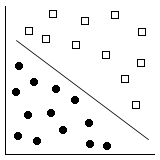
\includegraphics[scale=0.5]{./img/linear_svm.png}
	  \caption{Datos clasificados mediante una Maquina de Vector Soporte Lineal}
	  \label{fig:svm}
	\end{figure}

      \subsubsection{Aprendizaje No Supervisado}
	  Los algoritmos de aprendizaje No Supervisado se caracterizan por aplicarse a conjuntos de datos a los cuales, durante la etapa de entrenamiento no se les conoce su etiqueta
	  de salida, es decir, a diferencia de los algoritmos de aprendizaje supervisado, estos solo de los objetos para el entrenamiento, en lugar de disponer
	  de objetos y etiquetas. Estos algoritmos se emplean para detectar patrones o similaridades entre los datos que eran desconocidas.

	  Un ejemplo de esta clase de algoritmos es el algoritmo \emph{K-Means} empleado para el problema de Agrupamiento (Clustering en la literatura en inglés) de datos en distintas clases.
	  Este algoritmo consiste en reunir objetos de en K grupos, en el que cada observación es asignada al grupo para el cual su valor medio es mas cercano, ilustrado en la figura \ref{fig:clustering}.
	  De esta forma el concepto de distancia entre objetos cobra mucha importancia en este tipo de algoritmos.

	  \begin{figure}[H]
	    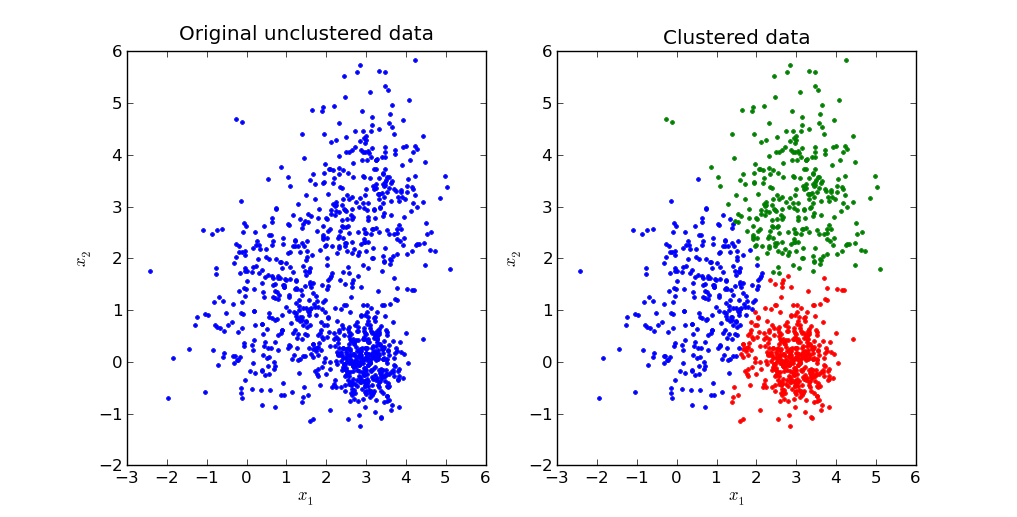
\includegraphics[scale=0.5]{./img/stackoverflow_clustering.png}
	    \caption{Datos no etiquetados agrupados mediante K-means}
	    \label{fig:clustering}
	  \end{figure}

      \subsubsection{Aprendizaje Semi-Supervisado}
	Estos algoritmos se caracterizan por utilizar una pequeña cantidad de datos etiquetados y otro gran conjunto de datos no etiquetados. Un ejemplo de esta clase de algoritmos
	es el filtrado colaborativo, utilizado para recomendar elementos a usuarios.

	El problema de recomendación consiste en tratar de predecir la preferencia que un usuario podría hacer por un artículo. El enfoque mayormente utilizado para realizar una
	recomendación es el de filtrado colaborativo, que se basa en la recolección y el análisis de una gran cantidad de información sobre los usuarios,
	los comportamientos, actividades o preferencias. La predicción de un posible articulo de interes para un usuario, se realiza basada en la similitud de este usuario con
	otros, de los cuales se les conoce mas información. Por ejemplo para recomendar una pelicula a un usuario, utilizando información de las peliculas ya observadas, se puede
	establecer una similtud de intereses con otros usuarios, que ademas vieron otras peliculas, las cuales son recomendadas a este usuario.

    \subsection{Representación de la Información en Aprendizaje Automático}
      Para que un modelo pueda aprender, es necesario lograr una representacion adecuada de los objetos sobre los cuales se desea asimilar información.
      Dependiendo de la información que se desee aprender, estas representaciones pueden ir variando. Si se desea entender sobre el riesgo crediticio de un usuario,
      la información que represente a este usuario sera diferente a la representación de ese mismo usuario si se desea  sobre sus intereses gastronomicos.

      Definir la representación de un objeto de forma precisa, tal que le permita al modelo capturar toda la información requerida puede llegar a ser la tarea mas importante de todo el 
      proceso de aprendizaje.
      Estas representaciones suelen estructurarse como un vector de características (\emph{features} en inglés) que el modelo deberá obtener a partir de las instancias de entrenamiento.
      Una \emph{feature} puede ser cualquier dato asociado a la instancia, que podría ser útil al modelo para realizar una predicción mas precisa.

      Por ejemplo para representar un conjunto de datos conformado por documentos de texto, el método comunmente utilizado es la bolsa de palabras (\emph{Bag of Words} en la literatura en inglés). 
      Este metodo emplea una estructura de datos auxiliar conocida como ``vocabulario'' o ``diccionario'', que contiene todas las palabras utilizadas en el conjunto de datos. 
      Cada documento se representa como un histograma de ocurrencias respecto de las palabras del vocabulario. 
      La dimensionalidad de la representación es igual al número de palabras que componen dicha estructura.

      Para representar una imagen, el método más sencillo es usar directamente el valor de los píxeles. No obstante, para que una representación de una imagen sea lo suficientemente
      descriptiva respecto al contenido de la misma, debe superar ciertos desafios, ilustrados graficamente en la figura \ref{fig:stanford_challenges}:
      \begin{itemize}
	\item Variación del punto de vista: Una simple instancia de un objeto puede estar orientada de muchas formas frente a la camara que toma la imagen.
	\item Variación de escala: Las clases visuales suelen exhibir variaciones en su tamaño en el mundo real y no solo en lo referido a la imagen.
	\item Deformación: Muchos objetos de interes no tienen un cuerpo rigido y pueden ser deformados de muchas formas
	\item Oclusión: Los objetos de interes pueden estar ocluidos y solo una pequeña porcion del objeto puede ser visible.
	\item Condiciones de iluminación: Los efectos de la iluminación pueden influir de forma drástica a nivel de píxeles.
	\item Influencia del fondo: los objetos de interés pueden estar inmersos en un ambiente en el cual sean dificiles de identificar.
	\item Variaciones intra clase: Existen muchos instancias completamente distinta de una misma categoría de objetos.
      \end{itemize}
      
      \begin{figure}[h]
	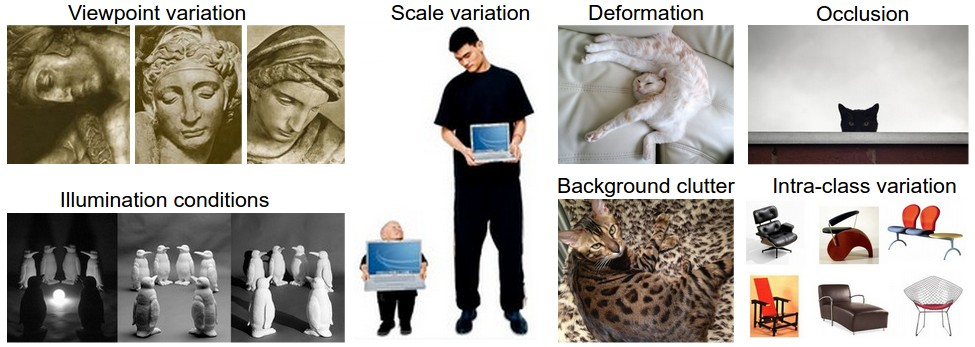
\includegraphics[scale=0.5]{./img/stanford_challenges.jpeg}
	\caption{Desafios que debe superar la representación de una imagen}
	\label{fig:stanford_challenges}
      \end{figure}

      A lo largo del desarrollo de la visión por computadora se distinguen dos enfoques para la generación de representaciones que permitan reconocer características de una imagen:
      El enfoque basado en técnicas superficiales (o “shallow” en inglés) y el enfoque de aprendizaje profundo (o “deep” en inglés).

      \subsubsection{Enfoque Clásico}
	En el enfoque clásico (o arquitecturas Shallow, como se conocen en la literatura en ingles), se busca generar una representación invariante a la posición, iluminación, fondo, etc.
	que describan regiones locales de la imagen, de forma robusta. Para ello se utilizan principalmente técnicas estadísticas a partir de conocimiento anterior del objeto y del contexto,
	con lo cual dependen en cierta forma de una decisión manual de quien construye el algoritmo.
	El conjunto de estas representaciones locales se codifican y agregan en una representación vectorial de dimensionalidad fija, la cual se emplea como
        entrada a los algoritmos de aprendizaje subsiguientes. Un ejemplo de esta clase de representaciones es el modelo de bolsas de palabras
        visuales el cual, en analogía al modelo para texto, recurre a una estuctura auxiliar para construir un histograma de ocurrencias de
        ``palabras visuales''. Este concepto se ilustra en la figura \ref{fig:bovw} en donde se intenta reconocer un rostro,
	una bicicleta y una guitarra, basandose en las palabras visuales que contiene su ``Diccionario''.

	\begin{figure}[h]
	  \begin{center}
	    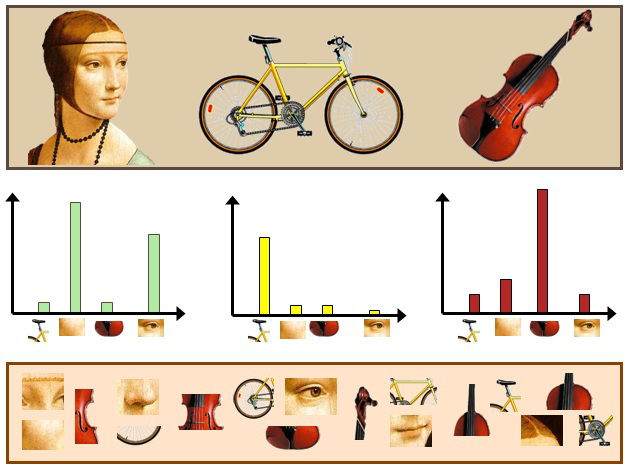
\includegraphics[scale=0.5]{./img/bag_of_visual_words.jpg}
	    \caption{Ejemplo de Bolsa de Palabras visuales}
	    \label{fig:bovw}
	  \end{center}
	\end{figure}

      \subsubsection{Enfoque de Aprendizaje Profundo}
	Este enfoque tiene como objetivo lograr una representación composicional de la imagen. Consta de un único algoritmo que, a diferencia del enfoque clasico, aprende a realizar 
	la representación por si mismo, en lugar de depender de decisiones externas.
	El contenido representado dependerá de la información que tenga como objetivo aprender el modelo. Por ejemplo, suponiendo que una misma imagen contenga un gato y un perro,
	si el modelo debe reconocer perros, la representacion contiene información relevante al perro, en cambio si el modelo debe reconocer animales, la representación incluye
	información de ambos animales.

	El problema asociado a este enfoque es que se desconoce cuales serán las \emph{features} que el modelo aprendera a representar durante el entrenamiento.
	Sin embargo, se puede establecer que las \emph{features} aprendidas tienen en cierto modo una especie de jerarquía, es decir que las \emph{features} de bajo nivel aprendidas desde los píxeles
	alimentan el aprendizaje de otras \emph{features} que aprenden a reconocer contornos y bordes, y así sucesivamente hasta llegar a las \emph{features} de mas alto nivel
	que logran reconocer estructuras y objetos. Debido a esto, las estructuras de aprendizaje profundo contemplan esta particularidad organizándose en diferentes capas,
	donde la salida de una capa es la entrada a la capa siguiente. Las Redes Neuronales Convolucionales soportan el aprendizaje de este tipo \emph{features}
	y es el modelo empleado en este trabajo. 

	En la figura \ref{fig:shallow_deep} se realiza una comparacion entre los enfoques clasicos y el enfoque de aprendizaje profundo.  En las 3 primeras opciones del diagrama se
	pueden observar las distintas formas de representar imágenes mediante técnicas de aprendizaje automático tradicional,
	donde, en todos los casos, las representaciones estan predefinidas antes de entrenar el modelo. Para mejorar estas representaciones se van agregando modulos 
	que permiten mejorar la prediccion.
	En cambio para las técnicas de aprendizaje profundo, las representaciones son directamente aprendidas durante el entrenamiento del modelo.

	\begin{figure}[h]
	  \begin{center}
		  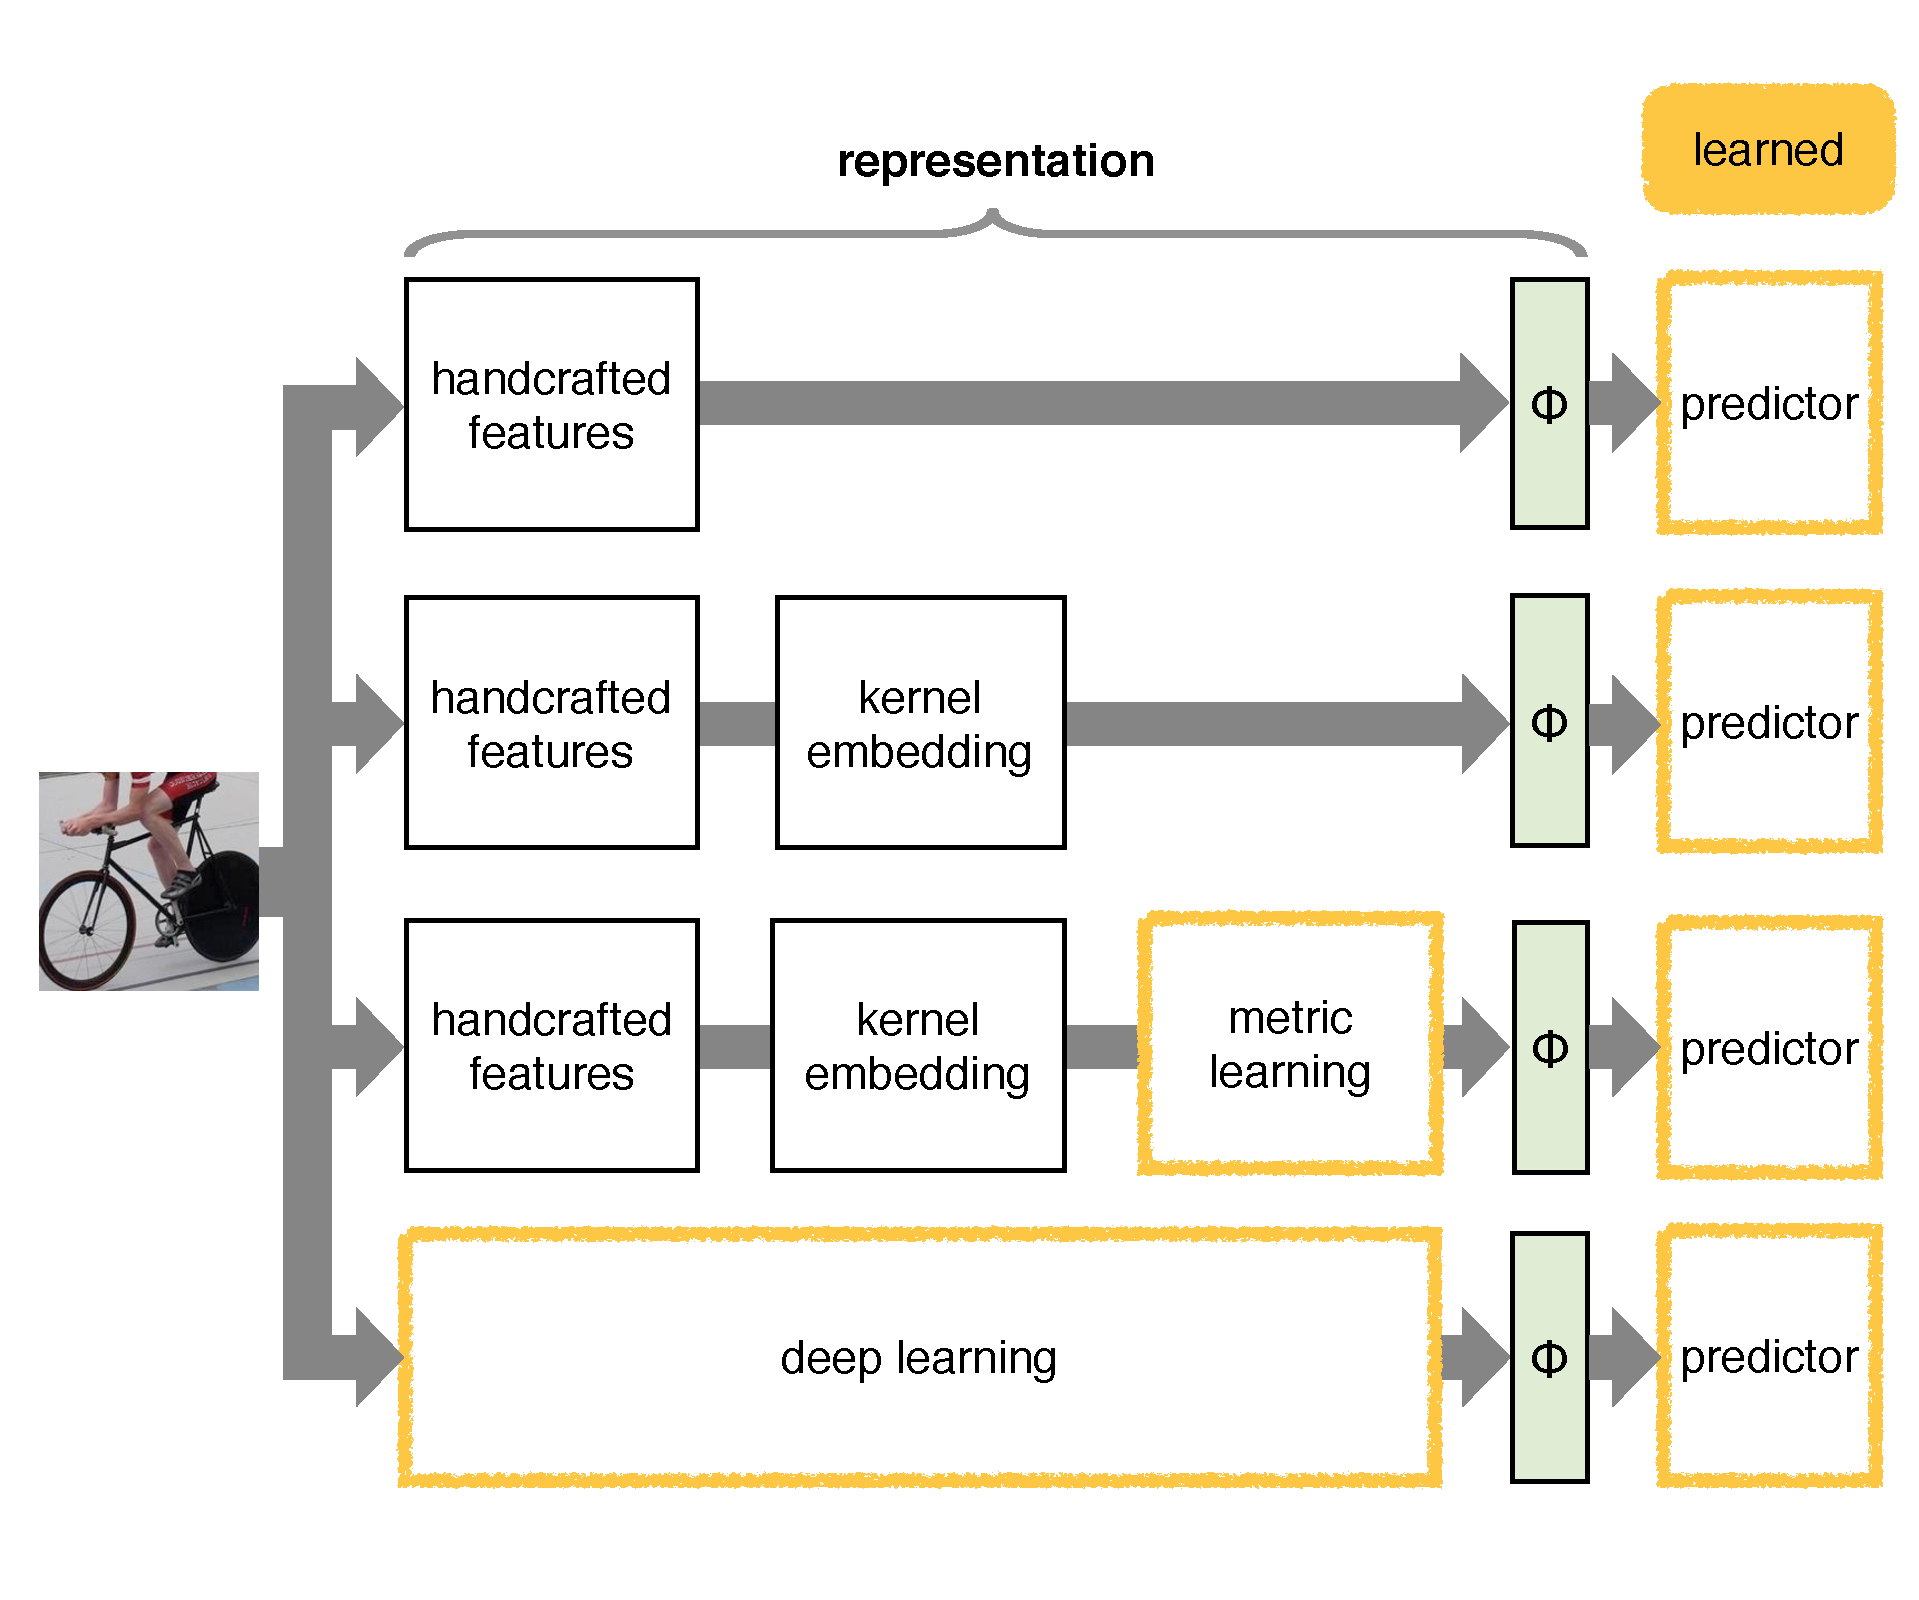
\includegraphics[width=0.9\linewidth]{./img/vedaldi_shallow_deep.pdf}
	  \caption{Comparacion de los distintos enfoques clasicos frente al enfoque de aprendizaje profundo}
	  \label{fig:shallow_deep}
	  \end{center}
	\end{figure}

        \subsection{Aprendizaje} \label{sec:aprendizaje}

	  Tanto en las representaciones ``shallow'' como en aquellas  basadas en arquitecturas ``deep'', el concepto de ``aprendizaje a
          partir de ejemplos'' requiere la introducción de dos conceptos fundamentales: el de función de predicción y el de función
          de perdida. Mediante la primera se define un modelo que, una vez ajustados sus parámetros, se utiliza para realizar predicciones sobre
          entradas no vistas durante el entrenamiento. La segunda define el criterio a partir del cual se deben ajustar los parámetros
          de la anterior. 
          
          Para facilitar la exposición, se abordará el problema de clasificación mediante funciones de predicción lineales. En la
          sección \ref{sec:redes_neuronales} se tratará el caso de funciones de predicción más complejas, en particular el caso de redes neuronales artificiales y
          sus particularidades.

	  Una función de predicción en clasificación se puede representar en términos generales como un mapeo $f_{\theta}: \mathcal{X}
          {\rightarrow} \{1,\dots,K\}$ con parámetros $\theta$, del conjunto del espacio de entrada $\mathcal{X}$ (en nuestro caso las imágenes o sus
          representaciones) al un conjunto discreto de categorías o clases ($\{1,\dots,K\}$). Al utilizar modelos lineales, la función de predicción toma la forma:
          \begin{equation} \label{eq:linear_classifier}
            f(x) = W x + b
          \end{equation}
          en donde $\theta=\{W, b\}$, con $W\in\mathbb{R}^{K \times D}$ y $b\in\mathbb{R}^K$.
          El objetivo del aprendizaje es estimar $\theta$, a partir de un conjunto de $N$ pares de entrenamiento $\{(x_i, y_i)\}_{i=1}^N$, $y_i \in \mathcal{X}$, $y_i\in\{1,\dots,K\}$
          donde $x_i$ hace referencia a la representación de la i-esima imagen del conjunto e $y_i$ es la respectiva categoría asociada.
	  A modo de ilustración, en la figura \ref{fig:linear_classifier} se puede observar graficamente como funciona un clasificador lineal que distingue aviones, autos y ciervos en imagenes.
	  \begin{figure}[ht]
	    \begin{center}
	     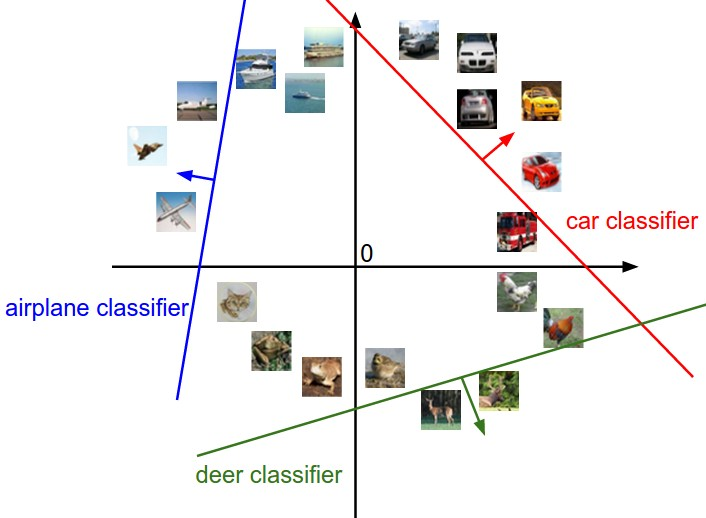
\includegraphics[width=0.8\linewidth]{./img/stanford_linear_class.jpeg}
	    \end{center}
	    \caption{Ejemplo de clasificador lineal que utiliza una función de puntuación lineal para clasificar entre autos, aviones y ciervos}
	    \label{fig:linear_classifier}
	  \end{figure}

\iffalse	  
	  Una predicción puede tener un resultado binario (0 o 1) o puede devolver un puntaje por lo general con valores continuos entre 0 y 1, indicando un cierto valor de confianza
	  de la predicción. Para el caso de un problema de clasificación de imágenes, el modelo dado una imagen, puede otorgar un puntaje a cada una de las $K$ clases posibles,
	  y la que obtenga el mayor puntaje será la clase asignada para esa imagen. Para poder realizar una predicción es necesaria una función de puntuación $f:R^D {\rightarrow} R^K$
	  donde $D$ es la dimensionalidad del vector de entrada (representación de la imagen) que toma $f$.

	  Además, es necesario una función de decisión $H$. Para el caso de clasificación $H:R^K{\rightarrow}\{1,..,K\}$ que toma el resultado de $f$ y decide a cual de las $K$ clases pertenece.
	  Un ejemplo de función de puntuación:
	  Suponiendo que tenemos $x$ una imagen de entrada, que la queremos asociar a una clase $y_{j}$ de las $K$ clases posibles , sea $D$ la dimensionalidad de $x$, $x \in R^D$,
	  $j \in 1..K$, entonces $f$ es una función: $f:R^D {\rightarrow} \{1,..,K\}$. El caso mas simple es el de una clasificador lineal, como se expresa en la ecuacion \eqref{eq:linear_classifier}.
	  \begin{equation}\label{eq:linear_classifier}
	    f(x, W, b) = W x + b
	  \end{equation}
	  Donde $W \in R^{K \times D}$, $b \in R^{K \times 1}$ son los parámetros de la función. 
	  Algunas cosas a tener en cuenta:
	  \begin{itemize}
	   \item Los datos de entrada $(x, y_{j})$  se consideran prefijados, pero los parámetros contenidos en $\theta$ son ajustables.
		 El objetivo del aprendizaje será establecerlos de tal manera que las puntuaciones computadas coincidan con las etiquetas correctas sobre todo conjunto de entrenamiento.
		 Intuitivamente, se desea que la clase correcta tenga una puntuación más alta que las puntuaciones de las clases incorrectas.
	   \item Una ventaja de este enfoque es que los datos de entrenamiento se utilizan para aprender los parámetros $W$ y $b$, pero una vez que el aprendizaje es completo,
		podemos descartar el conjunto de entrenamiento completo y sólo mantener los parámetros aprendidos, para evaluar una nueva instancia. Esto se debe a que una nueva imagen nunca vista puede ser
		simplemente reenviada a través de la función y clasificada en base a las puntuaciones computadas. En cambio, existen otros algoritmos de aprendizaje automático, que requieren
		mantener información de cada una de las instancias de entrenamiento para poder realizar la evaluación de una nueva instancia,
		como por ejemplo el algoritmo de K vecinos mas cercanos (\emph{K nearest neighbours} en la literatura en ingles).
	  \end{itemize}
\fi

	  El problema de estimar los parámetros de un modelo, se resuelve optimizando una función de costo expresada en la ecuacion \eqref{eq:perdida}.
          \begin{equation}\label{eq:perdida}
	    L = \frac{1}{N}\sum_{i=1}^{N} L_i(y_i, f(x_i, W, b)) + \lambda \Omega(W)
          \end{equation}
          Con $L:\mathcal{Y}\times \mathcal{Y}\rightarrow\mathbb{R}_+$, donde $\mathcal{Y}$ en el caso de la clasificación seria ${1,..,K}$.
          Esta ecuación contiene 2 términos: Un termino relacionado a las funciones de pérdida de cada imagen $L_i(y_i, f(x_i, W, b))$
          y un coeficiente de regularización $\lambda \Omega(W)$ que penaliza a los modelos complejos, $\lambda$ es un hiper-parámetro que define cuanto influye la regularización
          sobre el resultado final y $N$ es la cantidad de datos de entrenamiento.
	  Una función de pérdida es una función real, no negativa $L({\widehat y}, y)$, que mide cuán diferente es la predicción ${\widehat y}$ obtenida, con respecto a la
	  salida esperada $y$. Existen diversas funciones de pérdida que se utilizan en distintos contextos. A continuación se mencionan algunas que se aplican usualmente:
	  \begin{itemize}
	    \item Función de Pérdida 0-1:
	      \begin{equation*}
		L({\widehat y}, y) =  \begin{cases}
					    1 & \text{si ${\widehat y} = y$} \\
					    0 & \text{en caso contrario.}
		                      \end{cases}
	      \end{equation*}
	    \item Función de Pérdida Hinge:
	      \begin{equation*}
		L({\widehat y}, y) =  max(0, 1 - {\widehat y}y)
	      \end{equation*}
	      Esta funcion es ampliamente utilizada para algoritmos de Maquina de Vector Soporte, mencionados en la seccion \ref{sec:supervisado}.
	      Es una función convexa y continua pero no es derivable por lo tanto no se puede utilizar en métodos como el Descenso por el Gradiente.
	    \item Función de Pérdida Logística:
	      \begin{equation*}
		L({\widehat y}, y) =  {\log(1+ {\exp^{-{\widehat y}y}})}
	      \end{equation*}
	      Similar a la función Hinge, pero al ser derivable, puede utizarse para aplicar Descenso por el gradiente.
	    \item Función de Pérdida de Entropía Cruzada
	      \begin{equation} \label{eq:cross_entropy}
		L({\widehat y}, y) = -y{\log({\widehat y}}) - (1-y) {\log(1-{\widehat y})}
	      \end{equation}
	      Es una función continua, convexa y derivable que se adapta a métodos de Descenso por el gradiente, se utiliza en Redes Neuronales Profundas.

	  \end{itemize}
\iffalse
	\subsubsection {Sobreajuste y Regularización}
	  Uno de los principales objetivos de los algoritmos de aprendizaje automático es su capacidad de generalizar a ejemplos nunca antes vistos. Sin embargo, si la fase
	  de aprendizaje se realiza durante demasiado tiempo o si los ejemplos del conjunto de entrenamiento son raros, el modelo aprendido podría ajustarse específicamente
	  a ciertas características aleatorias de estos datos, que en realidad no contribuyen a la generalización. Esto se conoce como sobreajuste (overfitting en la literatura en inglés),
	  y es un problema importante y ampliamente discutido en el campo de aprendizaje automático. En el proceso de sobre ajuste, el desempeño del algoritmo en el
	  conjunto de entrenamiento sigue mejorando, pero en el conjunto de evaluación empeora.\\
	  Una técnica para evitar el sobre ajuste de modelos es utilizar regularización. Esencialmente, consiste en penalizar los parámetros del modelo para evitar su
	  crecimiento desmedido, agregando un regularizador($\Omega(W)$) a la Función de Pérdida. \\
	  La función de regularización mas comúnmente utilizada es la norma $L2$, definida como:
	   \begin{equation*}
	    \Omega(W) = \frac{1}{2} {\sum_{k} {\sum_{l}} W_{k,l}^2}
	   \end{equation*}
\fi
    \subsubsection{Optimización} \label{sec:optimizacion}
      Minimizar la función de pérdida \eqref{eq:perdida} puede considerarse un problema de optimización, con lo cual se pueden aplicar las técnicas empleadas en este tipo de problemas, para resolverlo.
      El objetivo de la optimización es encontrar el vector de pesos $W$ que minimice la función de pérdida.
      
      La estrategia de optimización mas utilizada para este tipo de problemas es la de seguir la dirección del gradiente (también llamado derivada) de la función de pérdida.
      En este caso que la función toma como entrada un vector de números, se aplican las derivadas parciales y el gradiente es el vector resultante de calcular las derivadas parciales
      en cada dimensión.La idea de principal de este método es el refinamiento iterativo, se evalúa el resultado del calculo del gradiente y se actualizan los parámetros repetidamente,
      toma un hiper-parámetro $\eta$ llamado tasa de aprendizaje que define el tamaño de cada paso en la iteración.
      Sea $F$ la función de pérdida, $w$ el vector de pesos, $N$ el numero de datos de entrenamiento, cada iteración consiste de:

      \begin{equation}\label{eq:gradient_descent}
	w_{n+1} = w_n - \eta \nabla L(w_n)  = w_n - \eta \sum_{i=1}^{N} \nabla L_i(w_n)
      \end{equation}

      Un problema recurrente en el aprendizaje automático es que para una buena generalización, son necesarios grandes conjuntos de entrenamiento,
      pero grandes conjuntos de entrenamiento también son más costosos desde el punto de vista computacional.
      En aplicaciones de gran escala, el conjunto de entrenamiento puede ser del orden de los millones de ejemplos, por lo que computar la función de
      pérdida completa sobre todo el conjunto para actualizar un solo parámetro, como ocurre en el caso de \eqref{eq:gradient_descent}, seria algo impracticable.
      
      Un enfoque común que se aplica a este problema es computar el gradiente sobre pequeños lotes del conjunto de entrenamiento,
      que permite lograr una buena aproximación al objetivo completo con una convergencia mucho mas rápida, es decir se reduce $N$ a un pequeño subconjunto, de esta forma se
      reduce el numero de cálculos realizados en cada iteración. Este método se lo conoce como \emph{Descenso por el gradiente estocástico} y es el mas utilizado para optimizar
      funciones de pérdida en las Redes Neuronales.

	\begin{algorithm}[ht]
	  \caption{Descenso por el gradiente estocástico}
	  \label{SGD}
	  \begin{algorithmic}
	    \State Elegir una tasa de aprendizaje $\eta$
	    \State Elegir un vector de pesos inicial $w_0$
	    \State Elegir un numero de iteraciones $J$
	    \State Ordenar aleatoriamente
	    \State $w \gets w_0$
	    \For{$j=1,..J$}
	      \ForAll {$i=1,..,N$}
		$sum_{gradiente} \gets sum_{gradiente} + \nabla L_i(w_n)$
	      \EndFor
	      \State $w \gets w - \eta sum_{gradiente}$
	    \EndFor
	  \end{algorithmic}
	\end{algorithm}
\iffalse
    \subsection{Resumen: Ciclo del Aprendizaje Automático}
      Luego de explicar todos los conceptos relevantes al Aprendizaje automático, podemos resumir al ciclo común a todos los algoritmos de Aprendizaje automático a lo siguiente:
      \begin{enumerate}
	\item Recopilación de datos:
	  El recopilado de datos es crucial, puede requerir mucho esfuerzo y cambio de procesos complejos,
	  Anotación, Muchas veces la clase objetivo tiene que ser calculada a mano por grupos de personas designadas para la tarea.
	\item Preprocesamiento de datos: Una vez obtenidos los datos, es necesario preprocesarlos para lograr tener datos limpios y útiles. Esta fase puede contener una etapa
	  de exploración y análisis, la cual permite conocer el dominio de donde provienen los datos.
	\item Definición de características: Para definir las características que el modelo debe aprender, en muchas ocasiones es necesario tener conocimiento del dominio a partir del cual provienen los datos.
	  La ingeniería de features ayuda a obtener características que provean información relevante a la hora de predecir.
	\item Entrenamiento:
	  \subitem Antes de comenzar el entrenamiento el conjunto de datos se divide en 2 subconjuntos, un conjunto de datos de entrenamiento y un conjunto de datos de prueba.
	  \subitem Para entrenar el modelo solo se utiliza el conjunto de datos de entrenamiento, el conjunto de datos de prueba se separa.
	  \subitem Determinar la estructura del modelo de aprendizaje, en base al tipo de problema y a la forma en la que se representan las características de los datos.
	  \subitem En algunos modelos, a partir del conjunto de datos de entrenamiento, se realiza otra partición de un pequeño subconjunto llamado conjunto de datos de validación, este conjunto sirve
	  para afinar ciertos hiper-parámetros del modelo.
	  \subitem Entrenar el modelo elegido sobre el conjunto de datos de entrenamiento
	\item Evaluación: Se aplica el modelo entrenado a los datos del conjunto de prueba, y se aplican métricas para poder establecer que tan bien predice el modelo entrenado para datos nunca antes vistos.
      \end{enumerate}



    \section{Clasificación de imágenes mediante Aprendizaje
      Supervisado}\FIXME{REMOVE. DEJARLO EN SUSPENSO PARA VER DONDE VA MÁS ADELANTE}
      \subsection{Introducción}
	La clasificación de imágenes es un problema que consiste en asignar a una imagen de entrada, una etiqueta de categoría a partir de un conjunto prefijado de categorias.
	Es uno de los principales problemas del area de visión por computadoras, pero que a pesar de su simplicidad tiene una gran cantidad y variedad de aplicaciones practicas,
	al punto de que otros problemas provenientes del area de visión por computadores pueden ser como detección de objetos o segmentacion pueden ser reducidos a clasificación de imágenes.
	El objetivo de presentar este problema es motivar el uso de las redes neuronales convolucionales en las siguientes secciones.
	\begin{figure}[h]
	  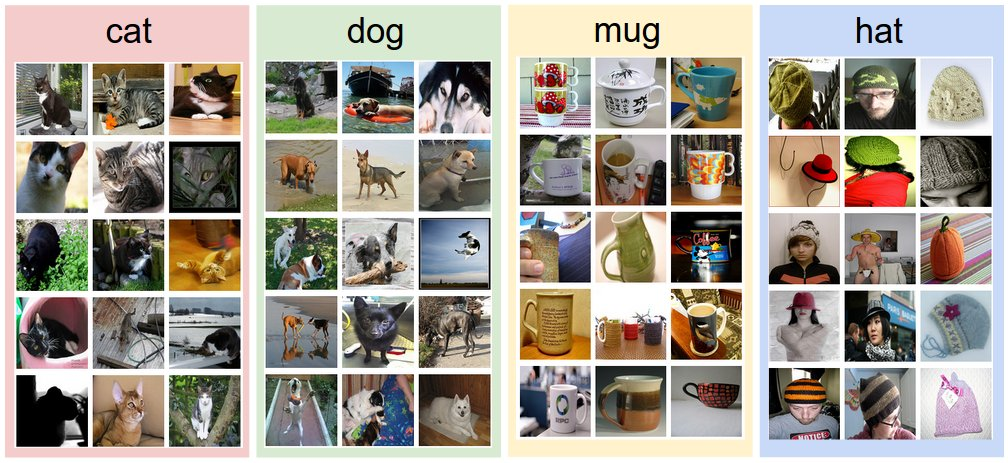
\includegraphics[scale=0.5]{./img/stanford_img_class.jpg}
	  \caption{Clasificación de imagenes en categorias: Perros, Gatos, Tazas y Gorros}
	  \label{fig:stanford_img_class}
	\end{figure}

	\subsubsection {Desafios}
	  Debido a que la tarea de reconocer un concepto visual es relativamente trivial para que lo realice una persona, vale la pena considerar los desafios involucrados desde la perspectiva de
	  un algoritmo de Visión por computadoras, teniendo en cuenta que la representacion pura de una imagen es un arreglo de 3 dimensiones que contiene valores de brillo. A continuacion de mencionan
	  algunos de los principales desafios
	  \begin{itemize}
	    \item Variación del punto de vista: Una simple instancia de un objeto puede estar orientada de muchas formas frente a la camara que toma la imagen.
	    \item Variación de escala: Las clases visuales suelen exhibir variaciones en su tamaño en el mundo real y no solo en lo referido a la imagen.
	    \item Deformación: Muchos objetos de interes no tienen un cuerpo rigido y pueden ser deformados de muchas formas
	    \item Oclusión: Los objetos de interes pueden estar ocluidos y solo una pequeña porcion del objeto puede ser visible.
	    \item Condiciones de iluminación: Los efectos de la iluminación pueden influir de forma drástica a nivel de píxeles.
	    \item Influencia del fondo: los objetos de interés pueden estar inmersos en un ambiente en el cual sean dificiles de identificar.
	    \item Variaciones intra clase: Existen muchos instancias completamente distinta de una misma categoría de objetos.
	  \end{itemize}
	  Un buen modelo de clasificación de imágenes debe ser tolerante a todos estos desafios presentados.
	  \begin{figure}[h]
	    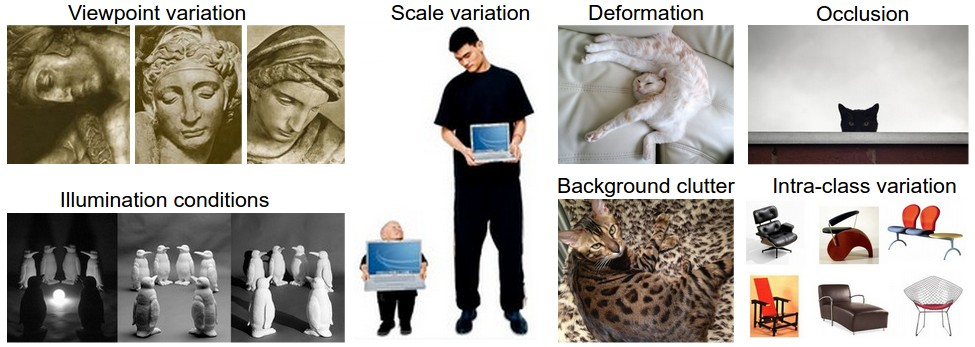
\includegraphics[scale=0.5]{./img/stanford_challenges.jpeg}
	    \caption{Aqui se pueden observar graficamente los desafios enumerados anteriormente}
	    \label{fig:stanford_challenges}
	  \end{figure}

	\subsubsection {Ciclo de Clasificación de Imágenes}
	  \begin{itemize}
	    \item Conjunto de datos de entrada: El conjunto de datos de entrada es un conjunto de N imágenes, cada una etiquetada con una de las K diferentes categorias.
	    \item Aprendizaje: En base al conjunto de datos de entrenamiento, el sistema debe aprender como identificar las caracteristicas de cada categoría para asi establecer un modelo clasificador.
	    \item Evaluación: Finalmente se evalua la calidad del modelo clasificador haciendo que prediga las etiquetas para un conjunto (de prueba) nuevo de imágenes que no habia visto antes, comparando las
	    etiquetas correctas con las etiquetas predecidas por el clasificador se puede establecer una metrica de calidad, intuitivamente se espera que las etiquetas predecidas coincidan en la mayoria
	    de los casos con las etiquetas correctas.
	  \end{itemize}
\fi


    \section{Redes Neuronales Artificiales}\label{sec:redes_neuronales}

      \subsection{Introducción}
	Un algoritmo de aprendizaje de red neuronal artificial, usualmente llamado ``red neuronal", es un algoritmo de aprendizaje que sirve como herramienta de modelado de datos
	en forma no lineal. Usualmente se usan para modelar relaciones complejas entre entradas y salidas,
	para encontrar patrones en los datos, o para capturar la estructura estadística en una distribución de probabilidad conjunta desconocida entre las variables observadas.
	Una red neuronal, basicamente es una version compleja del clasificador lineal, pero que utiliza los mismos conceptos de funciones de perdida y funcion de prediccion.
	  
	Las redes neuronales se pueden modelar como un conjunto de unidades de computo (neuronas) conectadas en un grafo acíclico, que se suelen organizar por capas, las neuronas de una capa
	se conectan con neuronas de sus capas adyacentes pero nunca se conectan 2 neuronas de una misma capa, como se puede observar en la figura \ref{fig:neural_network}.
	Toda red neuronal tiene una capa de entrada, una capa de salida y un número determinado de capas ocultas, que pueden ser de distintos tipos. En la caso de la figura \ref{fig:neural_network}
	la red neuronal que se ilustra, esta conformada por:
	\begin{itemize}
	 \item Una capa de entrada ($x_i$ con $i \in \{0,...,D\}$, donde $x_0$ corresponde al sesgo)
	 \item Una capa oculta ($z_m$ con $m \in {0,..,M}$ donde $z_0$ corresponde al sesgo). En el caso de que la red tenga mas de una capa oculta, $M$ puede ser distinto para cada una de ellas.
	 \item Una capa de salida ($y_j$ con $j \in \{1,...,K\}$)
	 \item Conexiones entre neuronas de capas adyacentes, las cuales contienen un peso $w^{(l)}_{se}$ donde $(l)$ es el numero de capa, $e$ es la neurona de entrada de la conexion y
	 $s$ la neurona de salida.
	\end{itemize}

	Una de las principales razones por la cual las redes neuronales están organizadas en capas, es que este tipo de estructura permite evaluar una red, muy simple y eficientemente realizando
	operaciones matriciales vectoriales, una red neuronal puede ser pensada como una serie de multiplicaciones de matrices entrelazadas con funciones de activaciones no lineales.
	Las redes neuronales utilizadas en la actualidad tienen alrededor de 100 millones de parámetros distribuidos entre 10-20 capas.

	\begin{figure}[ht]
	  \begin{center}
	    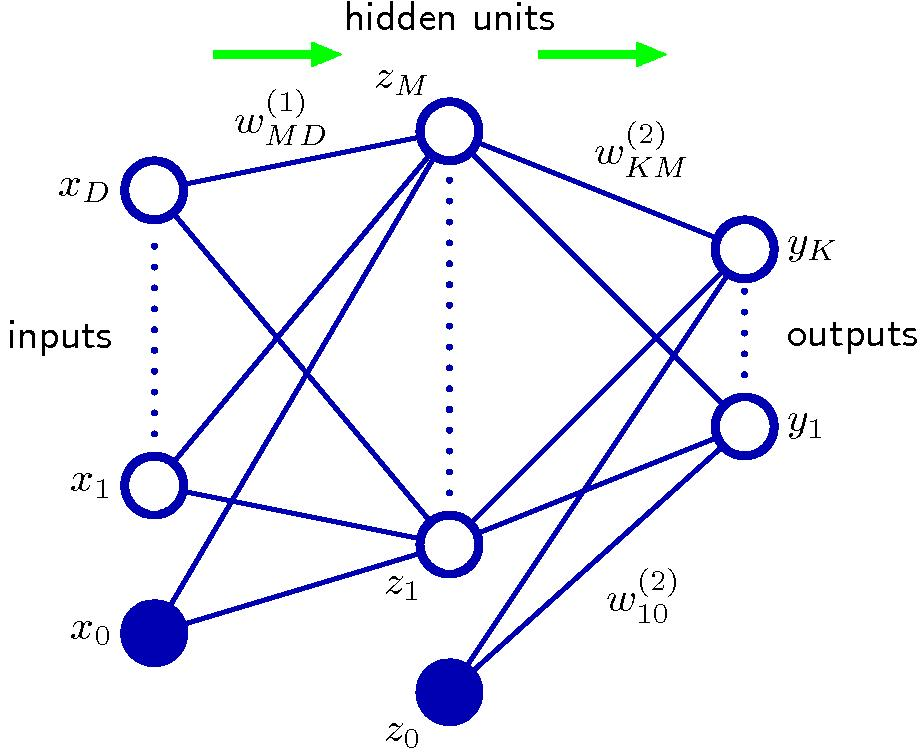
\includegraphics[width=0.8\linewidth]{./img/bishop_neural_network.jpg}
	  \end{center}
	  \caption{Red Neuronal Artificial}
	  \label{fig:neural_network}
	\end{figure}

	La unidad de procesamiento de una red neuronal es una neurona. La misma toma como parametros un vector de entrada, un vector de pesos, un valor de sesgo. El computo realizado
	en una neurona puede separarse en 2 etapas.
	\begin{enumerate}
	  \item En la primer etapa se realiza la suma de los productos punto a punto de los vectores de entrada, adicionandole finalmente el sesgo.
	    Sea $X$ el vector de entrada, de $D$ dimensiones, $W$ el vector de pesos y $w_0$ el sesgo, se puede formalizar de la siguiente forma:
	    \begin{equation} \label{eq:neurona_lineal}
	      a = \sum_{i=1}^{D} w_{i} x_i + w_{0}
	    \end{equation}
	    Donde $x_i$ es cada uno de los valores del vector $X$ y $w_{i}$ los valores del vector $W$. El valor $a$ se conoce como el valor de \emph{activación}.
	  \item En la segunda etapa se realiza una transformacion no lineal del valor de activación, obtenido en la etapa anterior, dada por la funcion de activación $h$,es decir:
	    \begin{equation}\label{eq:neurona_nolineal}
	      z = h(a)
	    \end{equation}
	\end{enumerate}
	La unidad aqui descripta pertenece a la primer capa oculta de la red, ya que en \eqref{eq:neurona_lineal} se interactua	con los valores del vector de entrada de la red, 
	en caso de que no pertenezca a la primer capa oculta, se reemplazan los $x_i$ por los correspondientes $z_i$
	obtenidos en la capa anterior. Finalmente cuando la unidad pertenece a la capa de salida, el valor obtenido en \eqref{eq:neurona_nolineal} termina siendo el valor de salida
	de la prediccion es decir $y$.
	
	Al utilizar una red neuronal como modelo de aprendizaje automatico para clasificación, primero es necesario configurar la arquitectura de la red para luego comenzar con la etapa de aprendizaje.

\iffalse
      \subsection{Aprendizaje basado en el Gradiente}
	El diseño y entrenamiento de una red neural no es muy diferente de la formación de cualquier otro modelo de aprendizaje automático con descenso por el gradiente.
	La diferencia más grande entre los modelos lineales y las redes neuronales es que la no linealidad de una red neuronal hace que las funciones de pérdida
	más interesantes se vuelvan no convexas. Esto significa que las redes neuronales suelen ser entrenadas mediante el uso de optimizadores iterativos basados ​​en gradientes
	que simplemente minimizan la función de costo, en lugar de los solucionadores de ecuaciones lineales usados ​​para entrenar modelos de regresión lineal. Para el caso de las
	redes neuronales, la técnica ampliamente utilizada es la de retropropagación del error que se detalla luego en la seccion \ref{sec:backpropagation}.
\fi

      \subsection{Configuracion y Diseño}
	En la etapa de configuracion y diseño de una red neuronal es donde se define la arquitectura de la red, es decir cuantas capas tendra, cuantas neuronas tendra cada una de las capas
	y cuales seran las funciones de activacion que estas utilizaran.
	Ademas en esta etapa se define cual sera la funcion de perdida que se utilizara para calcular el error durante el entrenamiento.

      \subsection {Aprendizaje}
	Una vez finalizada la etapa de configuracion y diseño es necesario inicializar los pesos, comunmente inicializados con valores aleatorios cercanos a 0, para luego comenzar con la etapa
	de entrenamiento de la red.
	El entrenamiento de una red neuronal consiste en realizar un ciclo de entrenamiento durante un cierto numero de iteraciones, utilizando el conjunto de datos de entrenamiento,
	de forma tal que se reduzca el error obtenido por la funcion de perdida, al comparar la predicción obtenida con el valor correcto de la etiqueta para esa instancia.
	El ciclo de entrenamiento se compone de 2 pasos: paso hacia adelante, y paso de retropropagación del error.
	\begin{enumerate}
	  \item En el paso hacia adelante se evalúa la red y se obtiene el resultado de salida, con el cual se mide el error, utilizando la función de perdida elegida.
	  \item En el paso de retropropagación del error se calcula el gradiente para luego ajustar los pesos internos de la red en base al resultado del gradiente,
	    desde las capas finales de la red hasta las capas iniciales.
	\end{enumerate}
	\begin{figure}[h]
	  \begin{center}
	  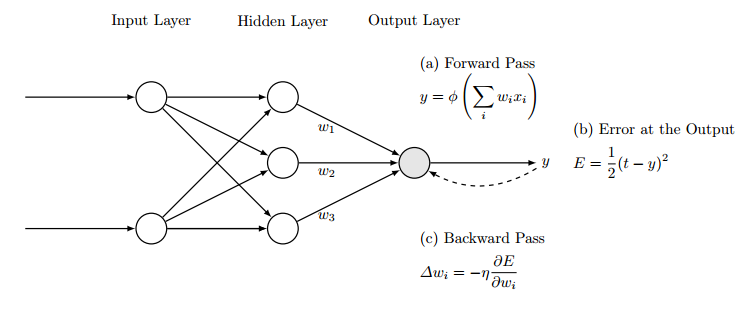
\includegraphics[width=0.8\linewidth]{./img/backprop.png}
	  \end{center}
	  \caption{ Descripción de la retropropagación. (a) El entrenamiento es alimentado hacia delante, generando de salida correspondiente. (b) Error entre la salida real y la salida deseada
	  se calcula. (c) El error se propaga hacia atrás, a través de actualizaciones donde una proporción del gradiente ($ \frac{\partial E}{\partial w_i}$ ) es la resta de cada peso. $x_i$, $w_i$, $\phi$ son las entradas,
	  la entrada de pesos, y la función de activación de una neurona. Error $E$ se calcula a partir de la salida $y$ de salida deseado $t$. $\eta$ es la tasa de aprendizaje.
	  \cite{Automatic_differentiation_ML} }
	  \label{fig:backprop}
	\end{figure}

      \subsection{Retropropagación del Error} \label{sec:backpropagation}
	La mayoría de los algoritmos de aprendizaje implican un procedimiento iterativo para la minimización de una función de perdida o error, en el cual ajustan los pesos mediante
	una secuencia de pasos. En cada paso, se pueden distinguir dos etapas bien diferenciadas. En la primera etapa, las derivadas de la función de error con
	respecto a los pesos deben ser evaluados. En la segunda etapa, las derivadas son utilizadas para calcular los ajustes que se les deben efectuar a los pesos, en cada una
	de las capas de la red. La importante contribución de la retropropagación (propagar el error hacia atras, a traves de la red) es la de proveer un
	método computacionalmente eficiente para evaluar las derivadas requeridas en la primer etapa. A lo largo de esta sección, iremos desarrollando las ideas fundamentales de dicho
	método.

	Como hemos visto, la función de perdida total, definida en \eqref{eq:perdida} se calcula midiendo el error en cada una de las $N$ instancias pertenecientes al conjunto de datos.
	Una forma simplificada de considerar \eqref{eq:perdida} es:
	\begin{equation} \label {eq:perdida_simplificada}
	  L(W) = \frac{1}{N}\sum_{n=1}^{N} L_n(Y_n, f(X_n, W)) + \lambda \Omega(W)
	\end{equation}
	donde el sesgo $b$ se considera parte del vector $W$. Ademas, como $(X_n, Y_n)$ estan predefinidas, podemos considerar que cada $L_n$ solo depende de $W$.
	Debido a todo esto, para calcular el gradiente de la funcion de perdida total, debemos evaluar $\nabla L_n(W)$ para cada término en la función de error. 
	Esto puede ser usado directamente para la optimización secuencial,o los resultados pueden ser acumulados a lo largo  del conjunto de entrenamiento en el caso de los métodos de optimización por lotes.
	
	Consideremos, en primer lugar de un simple modelo lineal en el que las salidas $y_k$ son combinaciones lineales de las variables de entrada $x_i$, es decir:
	\begin{equation*}
	  y_k = \sum_i W_{ki} x_i
	\end{equation*}
	Por simplicidad de decidió utilizar la función error cuadratica medio, que aunque no aplica para el caso de clasificación, facilita los calculos y puede
	ser reemplazada facilmente por otras funciones de error como por ejemplo Entropía Cruzada \eqref{eq:cross_entropy}. 
	Esta función para un determinado valor de entrada $n$, toma la forma:
	\begin{equation*}
	  L_n = \frac{1}{2} \sum_k (y_{nk}-Y_{nk})^2   % log-loss
	\end{equation*}
	donde $y_{nk} = y_{k} (X_n , W)$.
	
	El gradiente de esta función de error con respecto a un peso $w_{ji}$ está dada por:
	\begin{equation*}
	  \frac{\partial L_n}{\partial w_{ji}} = (y_{nj} − Y_{nj}) x_{ni}
	\end{equation*}
	que puede ser interpretado como un 'computo local' que involucra el producto entre un "error" $y_{nj} − Y_{nj}$ asociado a la de salida del enlace $w_{ji}$ y la variable $x_{ni}$
	asociada a la variable de entrada del enlace.
	Veremos ahora cómo este simple resultado se extiende hasta el escenario más complejo de redes neuronales artificiales.

	En una red neuronal cada unidad de computo, calcula una suma pesada de sus valores de entrada, de la forma:
	\begin{equation} \label{eq:unidad_computo}
	  a_j = \sum_{i} w_{ji} z_i
	\end{equation}
	Donde $z_i$ es el valor de entrada, $a_j$ es el valor que le envia a la unidad $j$ y $w_{ji}$ es el peso asociado a esa conexion.
	La suma obtenida en \eqref{eq:unidad_computo} es luego transformada por una funcion no lineal $h(.)$ para calcular el valor correspondiente a la unidad $j$, es decir:
	\begin{equation}\label{eq:nolineal}
	  z_j = h(a_j)
	\end{equation}
	Para cada instancia en el conjunto de entrenamiento, vamos a suponer que hemos suministrado el correspondiente vector de entrada a la red y que se calcula la activación
	de todas unidades en la red mediante aplicaciones sucesivas de \eqref{eq:unidad_computo} y \eqref{eq:nolineal}. Este proceso a menudo se denomina
	propagación hacia adelante porque puede ser considerado como un flujo de avance de la información a través de la red.
	
	Ahora, considere la evaluación de la derivada de $L_n$ con respecto a un peso $w_{ji}$. Los valores de salidas de las distintas unidades dependerá del vector de entrada $n$.
	Sin embargo, en el fin de mantener la notación despejada, vamos a omitir el subíndice $n$ de las variables de red. Primero observamos que $L_n$ depende del peso $w_{ji}$
	sólo a través de la suma de entrada $a_j$ a la unidad $j$. Por lo tanto, podemos aplicar la regla de la cadena para derivadas parciales, con lo cual obtenemos:
	\begin{equation} \label{eq:partial_derivatives}
	  \frac{\partial L_n}{\partial w_{ji}} = \frac{\partial L_n}{\partial a_j} \frac{\partial a_j}{\partial w_{ji}}
	\end{equation}
	Se introduce una notacion util:
	\begin{equation} \label{eq:notation}
	  \delta_j \equiv \frac{\partial L_n}{\partial a_j}
	\end{equation}
	Utilizando \eqref{eq:unidad_computo} podemos escribir:
	\begin{equation} \label{eq:sustitution1}
	  \frac{\partial a_j}{\partial w_{ji}} = z_i
	\end{equation}
	Substituyendo \eqref{eq:notation} y \eqref{eq:sustitution1} en \eqref{eq:partial_derivatives} obtenemos:
	\begin{equation} \label{eq:sustitution2}
	  \frac{\partial L_n}{\partial w_{ji}} = \delta_j z_i
	\end{equation}
	La ecuación \eqref{eq:sustitution2} nos dice que la derivada se obtiene simplemente multiplicando el valor de $\delta$ para la unidad en el extremo de salida del peso
	por el valor de$z$ para la unidad en el extremo de entrada del peso. Tenga en cuenta que esto lleva de la misma forma como para el simple modelo lineal considerado al inicio de esta sección.
	Por lo tanto, con el fin de evaluar los derivados, sólo tenemos que calcular el valor de $\delta_j$ para cada unidad oculta y de salida  en la red y, a continuación, aplicar \eqref{eq:sustitution2}.
	Dado que para las unidades de salida  utilizamos el enlace canonico \FIXME{REVISAR}, tenemos
	\begin{equation} \label{eq:delta_salida}
	  \delta_k = y_k - Y_k
	\end{equation}
	Para evaluar las $\delta$ para las unidades ocultas, volvemos a hacer uso de la regla de la cadena para derivadas parciales:
	\begin{equation}\label{eq:chain_rule}
	  \delta_j \equiv \frac{\partial L_n}{\partial a_j} = \sum_k \frac{\partial L_n}{\partial a_k} \frac{\partial a_k}{\partial a_j}
	\end{equation}
	
	\begin{figure}[ht]
	  \begin{center}
	  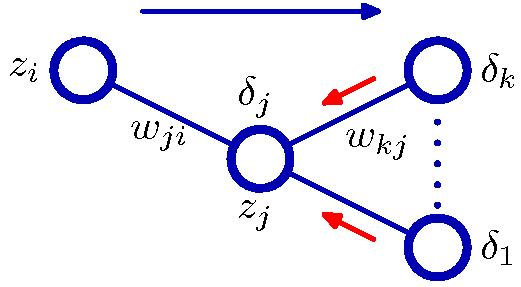
\includegraphics[width=0.5\linewidth]{./img/bishop_backpropagation.jpg}
	  \end{center}
	  \caption{Ilustración del cálculo de $\delta_j$ de la unidad oculta  $j$ por retropropagación de la $\delta 's$ a partir de las $k$ unidades para las cuales la unidad $j$ envía
	    conexiones. La flecha azul indica el la dirección del flujo de la información durante la propagación hacia adelante, y las flechas rojas indican la propagación
	    hacia atrás de la información de error.}
	  \label{fig:backpropagation}
	\end{figure}
	
	Donde la suma se ejecuta sobre todas las unidades $k$ donde la unidad $j$ envía conexiones. La disposición de las unidades y pesos se ilustra en la Figura \ref{fig:backpropagation}
	Notar que las unidades etiquetadas k podrían incluir otras unidades ocultas y/o de salida. En la escritura de la ecuacion \eqref{eq:chain_rule}, estamos haciendo uso del hecho
	de que las variaciones en un j dan lugar a variaciones en la función de error sólo a través de las variaciones en las variables de k. Si ahora sustituimos la definición
	de $\delta$ dada por \eqref{eq:notation} dentro de \eqref{eq:chain_rule}, y hacemos uso de \eqref{eq:unidad_computo} y \eqref{eq:nolineal}, obtenemos la siguiente fórmula de retropropagación
	\begin{equation}\label{eq:backpropagation}
	  \delta_j = h'(a_j) \sum_k w_{kj} \delta_k
	\end{equation}
	donde $h'$ es la función derivada a partir de $h$. La ecuacion \eqref{eq:backpropagation} nos dice que el valor de $\delta$ para una determinada unidad oculta se puede obtener mediante la propagación de la $\delta$'s hacia atrás a partir de unidades
	de más adelante en la red, como se ilustra en la figura \ref{fig:backpropagation}.
	Como ya conocemos los valores de los $\delta$'s para las unidades de salida, podemos aplicar de forma recursiva \eqref{eq:backpropagation} para evaluar los $\delta$'s
	para todas las unidades ocultas en una red, independientemente de su arquitectura.
	Por lo que la retropropagación del error se puede resumir en los siguientes pasos:
	\begin{enumerate}
	  \item Aplicar un vector de entrada $x_n$ a la red y  propagarlo hacia adelante a través de la red utilizando \eqref{eq:unidad_computo} y \eqref{eq:nolineal} para encontrar
	  las activaciones de todas las unidades ocultas y de salida.
	  \item Evaluar las $\delta_k$ para todas las unidades de salida utilizando \eqref{eq:delta_salida}.
	  \item Propagar hacia atras los $\delta$'s usando \eqref{eq:backpropagation} para obtener el $\delta_j$ de cada unidad oculta de la red.
	  \item Utilizar \eqref{eq:sustitution2} para evaluar las derivadas requeridas.
	\end{enumerate}

	\subsection {Funciones de Activación comúnmente utilizadas}
	  Como hemos visto en la seccion \ref{sec:redes_neuronales}, cada unidad de computo requiere de una funcion de activacion, la toma un único número como entrada,
	  realiza un operación matemática predefinida, no lineal y devuelve el resultado obtenido. En esta seccion se analizan las principales funciones de activacion utilizadas.
	  \subsubsection {Sigmoide}

	    La función sigmoide proyecta el dominio al rango (0,1) y su ecuación es:
	    \begin{equation*}
	     f(x) = \frac{1}{1+\exp^{-x}}
	    \end{equation*}
	    Ha tenido un uso frecuente desde el punto de vista histórico, ya que tiene una interpretación similar a la tasa de activación de una neurona:
	    de no activarse en absoluto (0) a activarse completamente a una frecuencia máxima asumida (1), como puede observarse en la figura \ref{fig:sigmoid}. En la práctica, la función sigmoide recientemente ha dejado de utilizarse,
	    ya  que tiene dos inconvenientes principales:
	    \begin{itemize}
	     \item Se satura y anula el gradiente. Una propiedad muy indeseable de la sigmoide es que cuando la activación de la neurona se satura en cualquiera de las dos puntas de 0 o 1,
	      el gradiente en estas regiones es casi cero. Esto hace que en la retropropagación, la información deje de retropropagarse hacia atras, (cuando se topa con un gradiente 0, cualquier
	      valor multiplicado por 0 es 0).
	     \item Las salidas no están centradas en cero. Esto es indeseable ya que las neuronas en capas posteriores de procesamiento en una Red Neuronal estarían recibiendo
	      datos que no están centrados en cero. Esto tiene implicaciones en la dinámica durante el descenso del gradiente, porque si los datos que llegan a una neurona
	      son siempre positivos, entonces el gradiente en los pesos durante la retropropagación o bien serán todos positivos o todos negativos.
	    \end{itemize}
	    \begin{figure}[ht]
	      \begin{center}
	       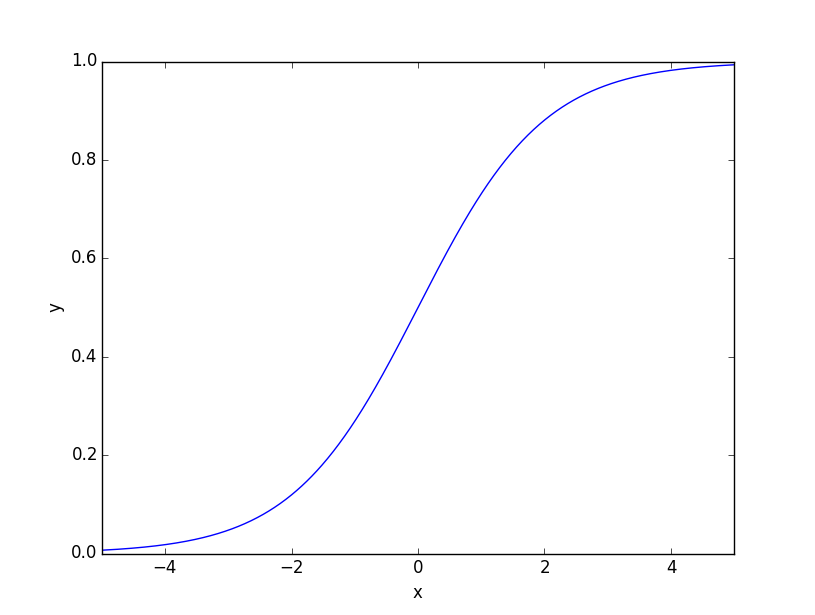
\includegraphics[width=0.4\linewidth]{./img/sigmoid.png}
	      \end{center}
	      \caption{Gráfico de la función Sigmoide}
	      \label{fig:sigmoid}
	    \end{figure}

	  \subsubsection {Tangente hiperbólica}
	    \begin{figure}[ht]
	      \begin{center}
	       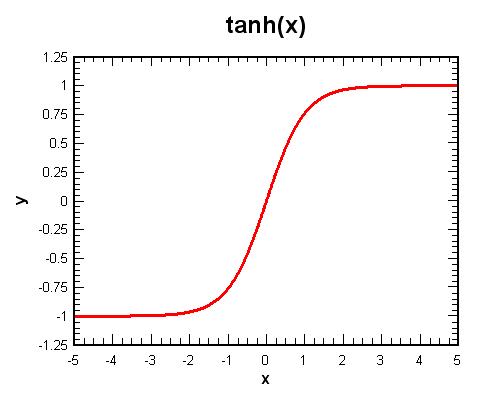
\includegraphics[width=0.4\linewidth]{./img/tanh.png}
	      \end{center}
	      \caption{Gráfico de la función Tangente hiperbólica}
	      \label{fig:tanh}
	    \end{figure}
	    Proyecta el dominio al rango [-1,1], como se muestra en la figura \ref{fig:tanh}. Al igual que la neurona sigmoide, sus activaciones saturan, pero a diferencia
	    de la neurona sigmoide su salida esta centrada en cero. Por lo tanto, en la práctica la tanh siempre es preferida sobre sigmoide.
	    \begin{equation*}
	     f(x) = \frac{\exp^x - \exp^{-x}}{\exp^x + \exp^{-x}}
	    \end{equation*}

	  \subsubsection {ReLU}
	    La Unidad Rectificada Lineal (Rectified Linear Unit en la literatura en inglés) se ha vuelto muy popular en los últimos años. Toma el máximo entre el valor y cero, es decir
	    simplemente le agrega un umbral igual a 0, su gráfico se puede ver en la figura \ref{fig:relu}.
	    \begin{equation}
	     f(x) = max(0,x)
	    \end{equation}
	    \begin{figure}[ht]
	      \begin{center}
	       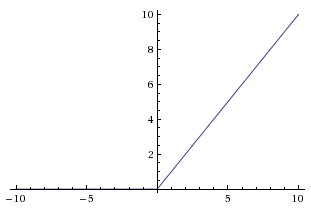
\includegraphics[width=0.4\linewidth]{./img/relu.jpeg}
	      \end{center}
	      \caption{Gráfico de la función ReLU}
	      \label{fig:relu}
	    \end{figure}

	    Las unidades lineales rectificadas son fáciles de optimizar porque son muy similares a las unidades lineales.
	    La única diferencia entre una unidad lineal y una unidad lineal rectificada es que una unidad lineal rectificada da salida a cero a través de la mitad de su dominio.
	    Esto hace que las derivadas a través de una unidad lineal rectificada permanezcan grandes siempre que la unidad esté activa.
	    Los gradientes no sólo son grandes sino también consistentes.

	    Algunas ventajas de utilizar ReLUs:
	    \begin{itemize}
	      \item Se encontró que aceleran en gran medida la convergencia del descenso del gradiente en comparación con las funciones sigmoides/tanh, esto se debe a su forma lineal, sin saturarse.
	      \item En comparación con las funciones tanh/sigmoide que implican operaciones caras, la ReLU puede implementarse simplemente marcando una matriz de activaciones a cero.
	    \end{itemize}

	    Existen varias generalizaciones de unidades lineales rectificadas. La mayoría de estas generalizaciones se comportan de forma comparable a las unidades lineales rectificadas
	    y, en ocasiones, tienen un mejor desempeño. Un inconveniente para las unidades lineales rectificadas es que no pueden aprender a través de métodos basados ​​en
	    gradiente en ejemplos para los cuales su activación es cero. Una variedad de generalizaciones de unidades lineales rectificadas garantizan que reciben gradiente en
	    todas partes. Existen generalizaciones sobre esta, que agregan un parámetro de regularización:
	    \begin{itemize}
	      \item Leaky ReLU: Agrega un parámetro de fuga $\alpha$, fijándolo en un valor pequeño como por ejemplo 0.01.
		\begin{equation}
		  f(x)=1(x<0)(\alpha x)+1(x>=0)(x)
		\end{equation}
	      \item ReLU Paramétrica: Trata el parámetro de fuga como un parámetro aprendible. \FIXME{AGREGAR FORMULA}
	    \end{itemize}

      \subsection {Regularización: Marginación}
	\FIXME{DESARROLLAR MAS, EXPLICAR COMO SE HACE, QUE EFECTO TIENE SI SACAMOS OVERFITING Y REGULARIZACION SACARLO}
	A la hora de definir la configuracion de una red, es posible agregar capas de marginación las cuales se emplean como
	técnica de regularización para reducir la saturación en redes neuronales previniendo el sobreajuste. Estas capas de marginación se encargan de
	\emph{silenciar} algunas neuronas, aleatoriamente, es decir toman valores de entrada, que para el caso de las neuronas elegidas a ser silenciadas, se ignoran
	sin generar valores de salida, como se puede observar en la figura \ref{fig:dropout}. Esto permite que durante el entrenamiento se evite el sobreajuste y la red aprenda
	a predecir correctamente aun sin disponer de toda la información, lo que termina produciendo una mejor generalización.
	\begin{figure}[ht]
	  \begin{center}
	   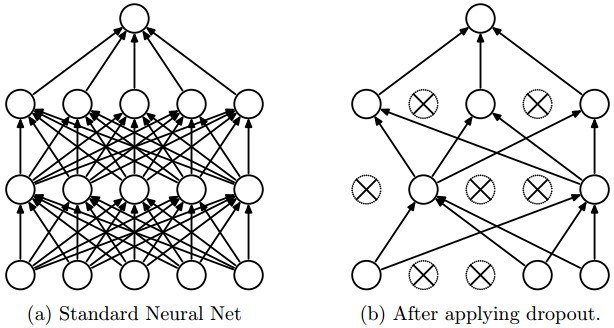
\includegraphics[width=0.6\linewidth]{./img/dropout.jpeg}
	  \end{center}
	  \caption{Durante el entrenamiento, la Marginación puede ser interpretada como tomar una subred Neuronal dentro de toda la Red Neuronal, y sólo actualizar los parámetros
	  de las subred basado en los datos de entrada. \cite{Srivastava:Dropout} }
	  \label{fig:dropout}
	\end{figure}
\iffalse
  \section {Aprendizaje Profundo}
    La caída de los precios de hardware y el desarrollo de GPUs para uso personal en los últimos años y la gran disponibilidad de datos, han contribuido al desarrollo del
    concepto de aprendizaje profundo (Deep Learning en ingles)
    que consiste de redes neuronales artificiales, que poseen mas de una capa oculta (se considera capa oculta a toda capa que no sea la de entrada ni salida). Este enfoque trata de
    modelar la forma en que el cerebro humano procesa luz y sonido en visión y audición.
    Algunas aplicaciones exitosas del aprendizaje profundo son la visión por computadora y el reconocimiento del habla.

    \subsection {Motivación}
      Los algoritmos simples de aprendizaje automático funcionan muy bien en una amplia variedad de problemas importantes.
      Sin embargo, no han logrado resolver los problemas centrales de Inteligencia Artificial, como reconocer el habla o reconocer objetos.
      El desafío de generalizar a nuevos ejemplos se vuelve más difícil cuando se trabaja con datos de gran dimensión y los mecanismos utilizados para lograr la generalización
      en el aprendizaje  automático tradicional son insuficientes para aprender funciones complicadas en espacios de alta dimensión.
      Tales espacios también suelen imponer altos costos computacionales. El aprendizaje profundo fue diseñado para superar estos y otros obstáculos.
\fi
  \section {Redes Neuronales Convolucionales} \label{sec:redes_convolucionales}
      Las redes neuronales convolucionales (Convolutional Neural Networks en ingles, o CNN) son muy similares a las redes neuronales antes vistas en la seccion \ref{sec:redes_neuronales}.
      La principal diferencia es que la arquitectura de una red neuronal convolucional asume explícitamente que el conjunto de entrada son imágenes. 
      Esto le permite codificar ciertas propiedades de las imagenes dentro de la arquitectura, obteniendo una mejor representación de las mismas.
      Están inspiradas en las redes neuronales tradicionales, incorporando operaciones no-lineales de manipulación de imágenes como la convolucion.
      
      En el area del procesamiento de imagenes, la convolución es una tecnica de proposito general para transferir el efecto a una imagen, utilizando el valor de sus pixeles,
      mediante una pequeña matriz comunmente llamada filtro (por lo general de $3\times3$ o $5\times5$).
      Al realizar la convolucion sobre una imagen, se aplica un filtro, obteniendo como resultado otra imagen nueva. Cada uno de los pixeles de esta nueva imagen se calcula de la siguiente forma:
      El filtro actua determinando el valor del pixel central donde se esta aplicando, sumando los valores de los pixeles vecinos pesados por el valor correspondiente de la matriz para
      cada pixel. En la figura \ref{fig:convolution}, se puede observar la aplicación de un filtro de $3\times3$. El caculo realizado es (40*0)+(42*1)+(46*0) + (46*0)+(50*0)+(55*0) + (52*0)+(56*0)+(58*0) = 42,
      por lo que el valor obtenido para ese pixel es 42.
      Este filtro se va desplazando sobre todos los pixeles de la imagen de entrada hasta lograr calcular el valor todos los pixeles de la imagen de salida. Para el caso de los pixeles 
      correspondientes a los bordes de la imagen, que no disponen de pixeles vecinos en alguna de las posiciones donde se aplica el filtro, existen diversas formas de completarlo. 
      Una forma de completar el calculo es considerando que donde hay pixeles ausentes su valor es cero, otra es considerar que tiene el mismo valor que el pixel mas cercano.
      \begin{figure}[h]
	\begin{center}
	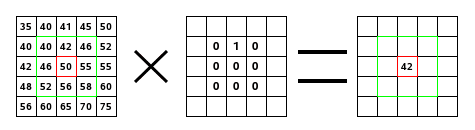
\includegraphics[width=0.8\linewidth]{./img/convolution.png}
	\end{center}
	\caption{Convolucion}
	\label{fig:convolution}
      \end{figure}

      Muchos de los enfoques modernos en Visión por Computadoras explotan la propiedad de que píxeles cercanos están más correlacionados entre ellos 
      que a los píxeles mas distantes. Esto se realiza mediante la extracción de características locales que dependen sólo pequeñas subregiones de la imagen. La información de tales características pueden entonces ser combinados
      en etapas posteriores de procesamiento con el fin de detectar de características de alto nivel hasta finalmente proveer información de la imagen completa. Además, las características
      locales que son útiles en una región de la imagen, probablemente sean útiles en otras regiones de la imagen.
      Estas nociones son incorporadas a las redes neuronales convolucionales mediante 3 mecanismos: (i) campos receptivos locales, (ii) compartir pesos y (iii) realizar submuestreos o agrupaciones.
      La estructura de una CNN se ilustra en la Figura \ref{fig:bishop_cnn}. En una capa convolucional, las unidades se organizan en 3 dimensiones, donde los distintos planos generados,
      utilizando la dimensiones alto y ancho se llaman mapa de caracteristicas.

      Las unidades en un mapa de caracteristicas toman como entradas solo una pequeña subregión de la imagen, y todas las unidades de un mismo mapa de caracteristicas se
      ven obligadas a compartir los mismos valores de peso. Por ejemplo, una mapa de caracteristicas puede consistir de 100 unidades dispuestas en una de cuadrícula 10x10,
      donde cada unidad  toma de entradas una porcion de 5x5 pixeles de la imagen. El mapa de caracteristicas completo tiene entonces 25 parametros de pesos ajustables,
      más uno de sesgo. Los valores de entrada de cada porcion de imagen son linealmente combinados utilizando los pesos y el sesgo, y el resultado es transformado por una funcion 
      no lineal como la funcion sigmoide.

      Si consideramos a las unidades como detectores de caracteristicas, entonces, todas las unidades en un mismo mapa de caracteristicas detectan el mismo patrón, pero en diferentes
      ubicaciones en la imagen de entrada. Debido a que comparten los pesos, la evaluación de las activaciones de estas unidades es equivalente a  realizar una operación de convolución
      sobre la intensidad de los pixeles de la imagen con un filtro compuesto por los parámetros de peso.
      
      \begin{figure}[h]
	\begin{center}
	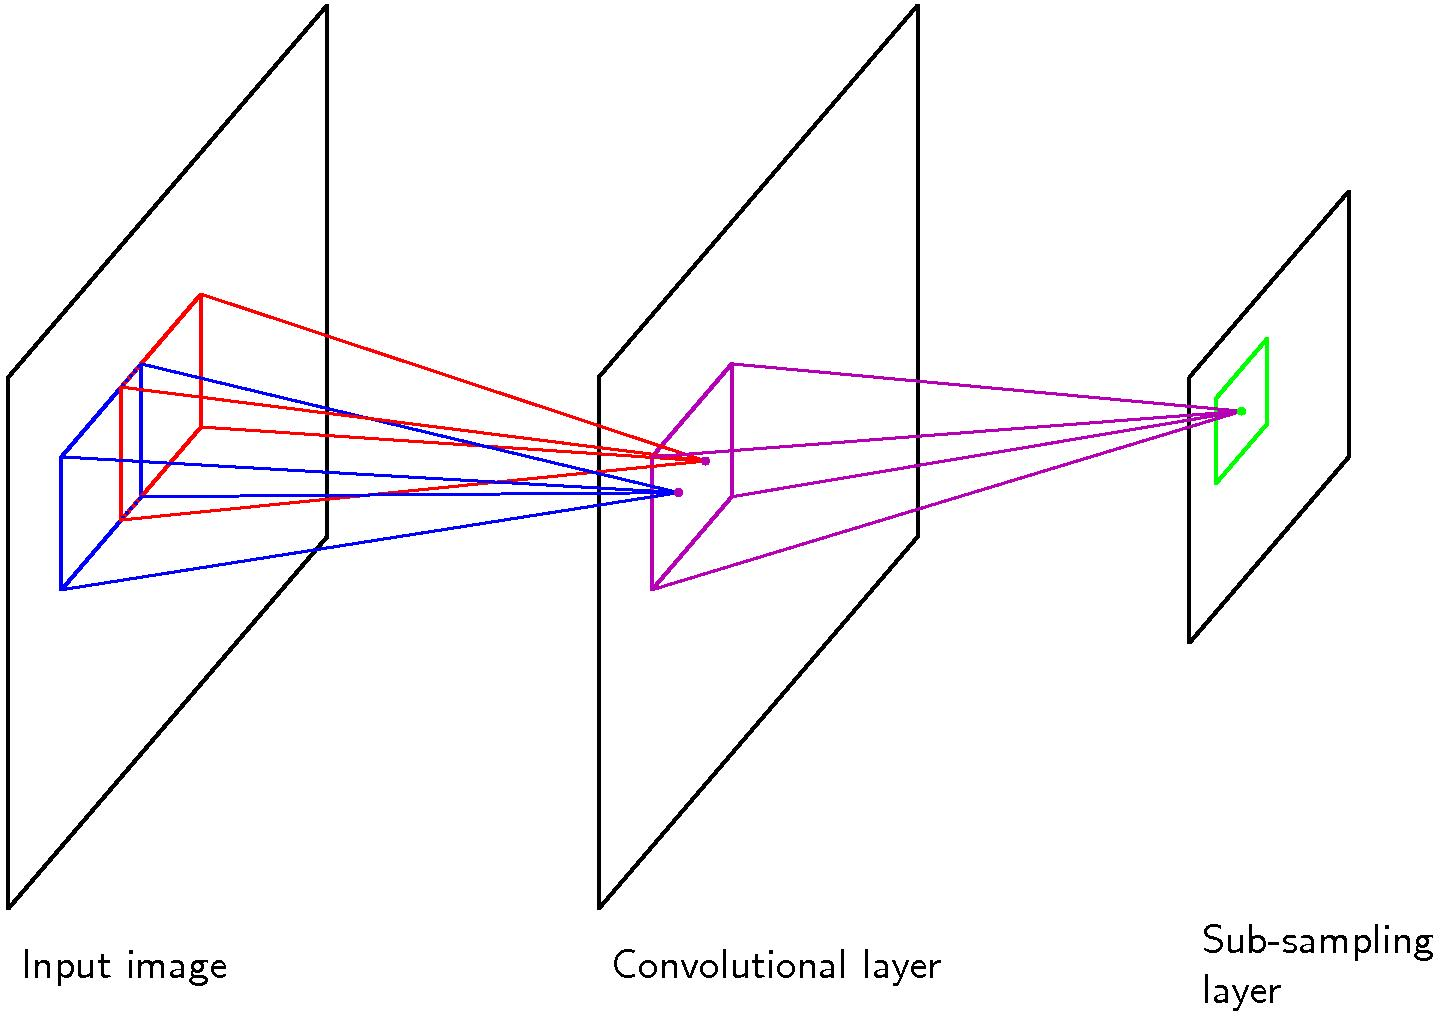
\includegraphics[width=0.8\linewidth]{./img/bishop_cnn.jpg}
	\end{center}
	\caption{Diagrama que ilustra parte de una CNN, mostrando una capa convolucional, seguido por una capa de agrupación.}
	\label{fig:bishop_cnn}
      \end{figure}
      
      Lograr diseñar una red convolucional que funcione correctamente, no es una tarea simple. Ademas, una red neuronal convolucional moderna requiere entre 2 y 3 semanas para entrenarse, 
      utilizando multiples GPUs para el conjunto de datos ImageNet \cite{imagenet_cvpr09}. Debido a estos motivos, en la actualidad un practica comun es adaptar
      redes famosas ya preentrenadas, realizando sobre estas ajuste fino (''Finetuning`` en la literatura en ingles), detallado en la seccion \ref{sec:finetuning}.

\iffalse
    \subsection {Arquitectura de una red neuronal convolucional}
      En las redes neuronales convolucionales, las unidades dentro de una capa se organizan en 3 dimensiones: alto, ancho y profundidad, como se ilustra en la figura \ref{fig:cnn}.
      Cada capa acepta un volumen de 3 dimensiones como entrada y lo transforma en un volumen de salida de 3 dimensiones a través de una función diferenciable.
      La entrada y salida de cada una de estas capas son conjuntos de arreglos llamados mapas de caracteristicas.
      En el caso mas simple de arquitectura, la red transforma el volumen de una imagen de entrada en un volumen de salida, conteniendo los puntajes de cada clase para el problema de clasificación.
      Típicamente, las CNNs suelen además organizarse por etapas, cada etapa consiste de una capa convolucional, una no lineal y una de agrupamiento.
      A continuación se detallan estos tipos de capas.
      \begin{figure}[H]
	\begin{center}
	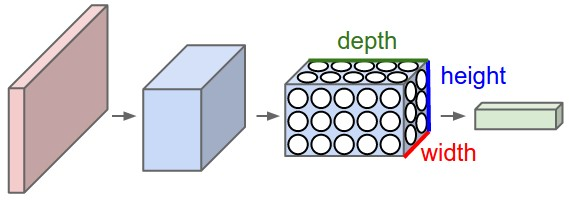
\includegraphics[width=0.8\linewidth]{./img/stanford_cnn.jpeg}
	\end{center}
	\caption{Una CNN ordena a sus neuronas en tres dimensiones (ancho, alto, profundidad), como se visualiza en una de
	  las capas. Cada capa de una CNN transforma un volumen 3D de entrada a un volumen 3D de salida. En este ejemplo, en la capa de entrada se encuentra la imagen, por lo que su ancho y su altura
	  serían las dimensiones de la imagen, y la profundidad sería 3 (los canales Rojo, Verde, Azul). \cite{Karpathy:Stanford}}
	\label{fig:cnn}
      \end{figure}
\fi

    \subsection {Tipos de Capas}
      \subsubsection{Capa Convolucional} \label{}
	Los parámetros consisten en un conjunto de filtros aprendibles. Cada filtro es pequeño espacialmente (alto y ancho) pero se extiende sobre toda la profundidad del volumen de entrada.
	Durante el paso hacia adelante, se desliza o convoluciona el filtro a través del alto y ancho del volumen de entrada y se computa el producto punto entre los valores del filtro y los valores
	del volumen de entrada. A medida que se va deslizando el filtro sobre el ancho y el alto del volumen de entrada, se va generando un mapa de caracteristicas de 2 dimensiones que contiene los
	valores de respuesta de ese filtro en cada posición espacial.

	Intuitivamente, la red aprenderá los filtros que se activan cuando ven algún tipo de característica visual como un borde de cierta orientación o una mancha de algún color en la
	primera capa, o eventualmente panal entero o patrones de rueda en las capas más altas de la red. Dado que tendremos un conjunto de filtros en cada capa Convolucional,
	y cada uno de ellos producirá un mapa de activación bidimensional separado, estos se apilaran a lo largo de la dimensión de profundidad para producir el volumen de salida.

	\begin{figure}[H]
	  \begin{center}
	   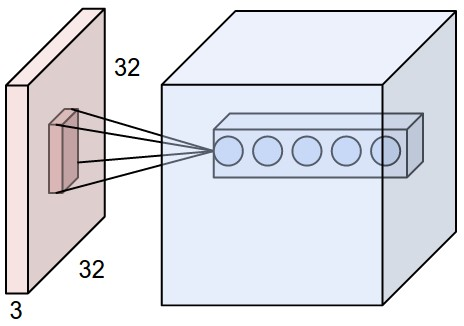
\includegraphics[width=0.8\linewidth]{./img/stanford_conv_layer.jpeg}
	  \end{center}
	  \caption{Un ejemplo del volumen de entrada (por ejemplo, un volumen de 32x32x3), y un ejemplo de volumen de neuronas en la primer capa Convolucional.
	    Cada neurona de la capa convolucional está conectada sólo a una región local en el volumen de entrada espacialmente, pero a la profundidad total (es decir, todos
	    los canales de color). Notar que hay múltiples neuronas (5 en este ejemplo) a lo largo de la profundidad, todos mirando en la misma región en la entrada.
	    A la derecha: Las neuronas de la Red Neuronal se mantienen sin cambios: Se calcula un producto punto de su peso con el de entrada seguido de una no-linealidad,
	    pero su conectividad está ahora restringida a ser local en el espacio. \cite{Karpathy:Stanford}}
	  \label{fig:conv_layer}
	\end{figure}

      \subsubsection{Capa de Agrupación}
	Su función es reducir progresivamente el tamaño espacial de la representación para reducir la cantidad de parámetros y de cálculo en la red, y por lo tanto también para controlar
	el sobreajuste. La capa de Agrupación (Pooling en la literatura en ingles) funciona independientemente en cada segmento de profundidad de la entrada y la redimensiona espacialmente, utilizando la operación de máximo,
	también se suele utilizar la operación de promedio o la norma L2.

	\begin{figure}[H]
	  \begin{center}
	   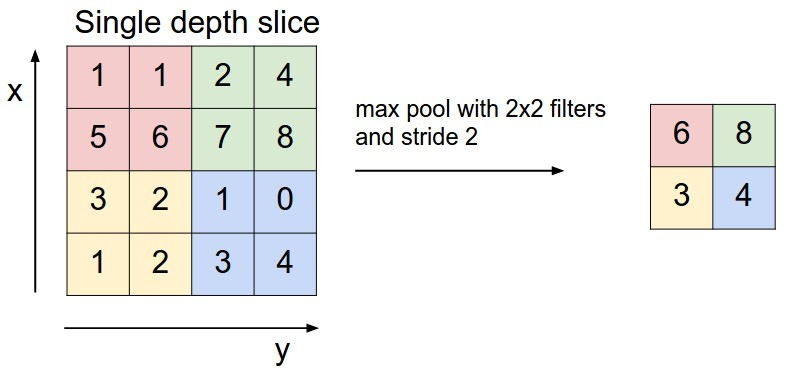
\includegraphics[width=0.8\linewidth]{./img/stanford_maxpool.jpeg}
	  \end{center}
	  \caption{La capa agrupación reduce el volumen espacialmente, de forma independiente en cada una profundidad de la entrada de volumen.
	    A la izquierda: En este ejemplo, el volumen de entrada de tamaño [224x224x64] es agrupado con un filtro de tamaño 2 y salto 2 en un volumen de salida de tamaño [112x112x64].
	    Observe que la profundidad del volumen se conserva. A la Derecha: la forma más común de reducción de tamaño de la operación de máximo, dando lugar agrupación por máximo,
	    que aquí se muestra, con un salto de 2. Es decir, cada operación se toma con 4 números (pequeño cuadrado de 2x2). \cite{Karpathy:Stanford}}
	  \label{fig:maxpool_layer}
	\end{figure}

      \subsubsection{Capa Completamente Conectada}
	Una capa completamente conectada toma todas las neuronas de la capa anterior y las conecta a cada una de las neuronas que posee, es decir,
	mediante una capa completamente conectada, las neuronas entre dos capas adyacentes están completamente conectadas de a pares, de esta forma, se pierde la localidad espacial,
	por lo que este tipo de capas suelen estar al final de la red.

    \section {Ajuste fino} \label{sec:finetuning}
      El ajuste fino (Finetuning en inglés), es una tecnica que toma un modelo ya entrenado, con sus respectivos pesos,  y consiste en adaptar la arquitectura
      del modelo inicial, para el problema al cual se quiere emplear, brindando un conjunto de datos de entrenamiento con el cual se entrena la red adaptada,
      pero la inicializacion de los pesos coincide con los pesos obtenidos del modelo preentrenado.
      Por ejemplo una red fue entrenada para reconocer distintas razas de perros en imagenes, y ahora se desea clasificar gatos segun su raza. En lugar de entrenar una
      red desde un estado aleatorio inicial, se puede utilizar la red preentrenada para perros, reemplazando la ultima capa completamente conectada por otra que
      tenga la cantidad de salidas igual a la cantidad de razas de gato que se desean reconocer.
      Para el entrenamiento de esta red adaptada se le da como entrada un conjunto de imagenes, de gatos de las distintas razas, de esta forma los  pesos se van
      ajustando para lograr reconocer este nuevo tipo de conceptos en las imagenes.
      
      \subsection{Redes Convolucionales Famosas y Modelos preentrenados} \label{sec:cnn_famosas}
	Como mencionamos anteriormente, una practica usual es reentrenar modelos preentrenados, adaptandolos a las necesidades especificas. Existen modelos de redes convolucionales
	que reconocidos por haber ganado competencias orientadas a la clasificacion de imagenes, los cuales son de disponibilidad publica. Estos modelos suelen ser empleados como base 
	preentrenada. A continuación se mencionan algunos de los mas famosos:
	
	\subsubsection{LeNet}
	  El primer éxito en las aplicaciones de Redes Neuronales Convolucionales, fue desarrollado por Yann LeCun \cite{Lecun:LeNet} en la década de 1990.
	  La aplicación mas conocida que utiliza la arquitectura LeNet es para leer los códigos postales, números, etc. Esta arquitectura es de las mas rudimentarias y 
	  solo contiene 5 capas de las cuales 2 son capas convolucionales como se ilustra en la figura \ref{fig:lenet}. 
	  
	  \begin{figure}[h]
	    \begin{center}
	    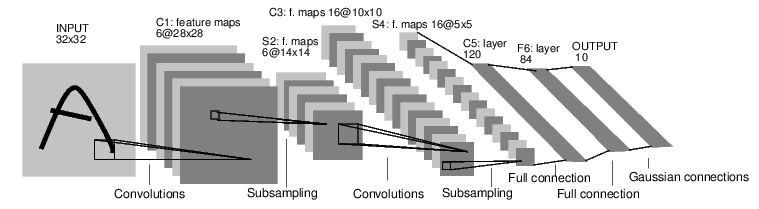
\includegraphics[width=0.6\linewidth]{./img/lenet.png}
	    \end{center}
	    \caption{Arquitectura de la red LeNet}
	    \label{fig:lenet}
	  \end{figure}

	\subsubsection{AlexNet}
	  La primera obra que popularizó las Redes Neuronales Convolucionales en Visión por Computadoras fue el AlexNet  \cite{AlexNet}, desarrollada por Alex Krizhevsky, Ilya Sutskever y Geoff Hinton.
	  La red AlexNet fue presentada al desafío ImageNet ILSVRC  en 2012 y obtuvo el primer puesto superando significativamente al segundo (top 5 de error de 16\% en comparación con el
	  subcampeón con el 26\% de error). La red tenía una muy arquitectura similar a LeNet, pero era más profunda, con más  capas convolucionales apiladas una encima de la otra
	  (anteriormente era común tener solo una capa convolucional siempre seguida inmediatamente por una capa de agrupación). La arquitectura de esta red se puede observar en la figura 
	  \ref{fig:alexnet}.
	  
	  \begin{figure}[h]
	    \begin{center}
	    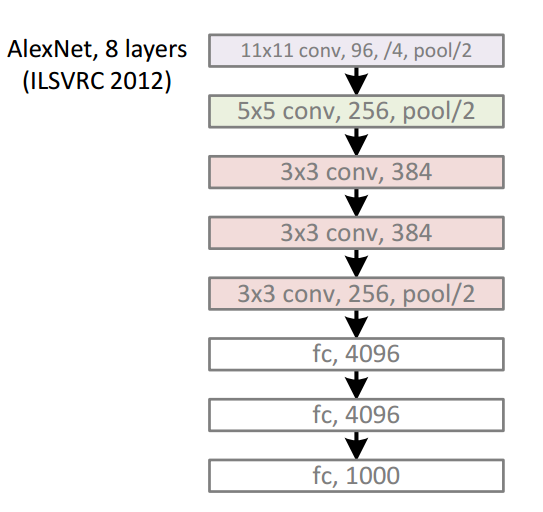
\includegraphics[width=0.6\linewidth]{./img/alexnet.png}
	    \end{center}
	    \caption{Arquitectura de la red AlexNet}
	    \label{fig:alexnet}
	  \end{figure}	  

	\subsubsection{GoogLeNet}
	  El ganador de ILSVRC 2014 fue la Red Convolucional de Szegedy \cite{Szegedy:Convolutions}, proveniente de Google. Su contribución principal fue el desarrollo de un 
	  módulo de ``Inception'' que reduce drásticamente el número de parámetros de la red (4M, en comparación con AlexNet con 60M). 
	  Este modulo basicamente actua como multiples filtros de convolucion
	  procesados sobre el mismo dato de entrada. Todos los resultados obtenidos son concatenados, lo cual le permite al modelo extraer caracteristicas de multiples niveles sobre
	  cada entrada. Por ejemplo puede extraer caracteristicas generales (filtros de 5x5) y locales (1x1) en el mismo momento. En la figura \ref{fig:inception} se ilustra la arquitectura
	  de este modulo graficamente.

	  \begin{figure}[h]
	    \begin{center}
	    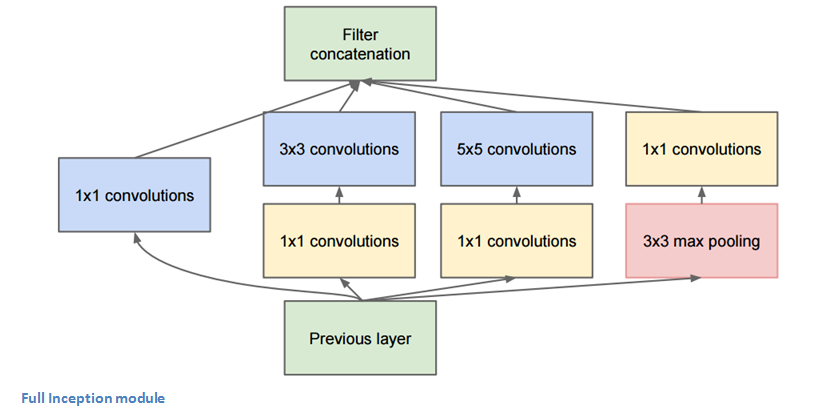
\includegraphics[width=0.6\linewidth]{./img/googlenet_inception_module.png}
	    \end{center}
	    \caption{Bloque ``Inception'' de la red GoogLeNet}
	    \label{fig:inception}
	  \end{figure}	  

	\subsubsection{VGG}
	  El segundo puesto en ILSVRC 2014 fue la red de Karen Simonyan y Andrew Zisserman que llegó a ser conocido como VGG \cite{SimonyanVGG}. 
	  Su contribución principal fue demostrar que la profundidad de
	  la red es un componente crítico para el buen desempeño. Su version final contiene 19 capas de las cuales 16 son convolucionales. Esta red ofrece una arquitectura 
	  muy homogénea, sólo realiza convoluciones de 3x3 y agrupaciónes de 2x2 desde el principio hasta el final, ilustrado en la figura \ref{fig:vgg}.
	  Una desventaja de la VGG es que es muy cara para evaluar y consume mucha memoria y parámetros (140M). La mayoría de estos parámetros se encuentran en la primera
	  capa totalmente conectada, y desde entonces se ha encontrado que estas capas pueden ser removidos con ningúna disminucion de rendimiento, reduciendo significativamente el
	  número de parámetros necesarios.
	  
	  \begin{figure}[h]
	    \begin{center}
	    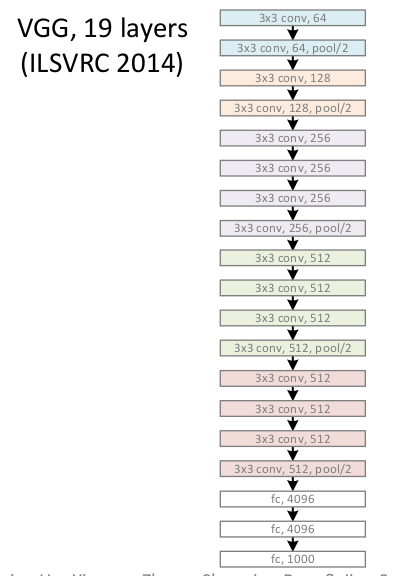
\includegraphics[width=0.6\linewidth]{./img/vgg-19.png}
	    \end{center}
	    \caption{Arquitectura de la red VGG}
	    \label{fig:vgg}
	  \end{figure}	

	\subsubsection{Resnet}
	  Las Redes Residuales (ResNet) fueron desarrolladas por Kaiming He \cite{Kaiming:ResNet}, que fue el ganador de ILSVRC 2015. La caracteristica particular de este tipo de redes 
	  es que utilizan bloques de conexiones salteadas ilustrados en la figura \ref{fig:resnet}. 
	  Esta arquitectura también solo tiene una capa completamente conectada en el extremo final de la red, en las capas intermedias hacen uso intensivo de la normalización por lotes.
	  En cuanto al numero de capas de la red, existen diversas versiones de las ResNet, algunas de las cuales llegan a tener mas de 150 capas.
	
	  \begin{figure}[h]
	    \begin{center}
	    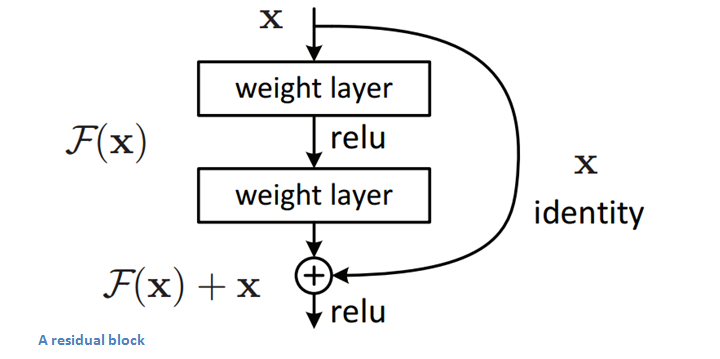
\includegraphics[width=0.6\linewidth]{./img/resnet_block.png}
	    \end{center}
	    \caption{}
	    \label{fig:resnet}
	  \end{figure}	
	
\iffalse
      \paragraph{Como y cuando hacer Reentrenamiento}
      \FIXME{REVISAR SI HACE FALTA PONERLO}
	¿Cómo decidir qué tipo de transferencia de aprendizaje debe realizar en un nuevo conjunto de datos? Esta es una función de varios factores, pero los dos más importantes son el
	tamaño del nuevo conjunto de datos (pequeño o grande), y su similitud con el conjunto de datos original (por ejemplo ImageNet-como en términos de contenido de imágenes y las clases,
	O muy diferentes, tales como imágenes de microscopio). Teniendo en cuenta que las características de CNN son más genéricas en capas tempranas y más específicas del conjunto de datos
	originales en capas posteriores, aquí hay algunas reglas comunes para navegar por los 4 escenarios principales:
	\begin{itemize}
	  \item El nuevo conjunto de datos es pequeño y similar al conjunto de datos original. Dado que los datos son pequeños, no es una buena idea afinar la red convolucional debido a las
	  preocupaciones excesivas. Dado que los datos son similares a los datos originales, esperamos que las características de mayor nivel en la red convolucional sean relevantes para este
	  conjunto de datos. Por lo tanto, la mejor idea podría ser la de formar un clasificador lineal utilizando las caracteristicas extraidas en la ultima capa de la red.
	  \item El nuevo conjunto de datos es grande y similar al conjunto de datos original. Dado que tenemos más datos, podemos tener más confianza de que no superaremos si intentáramos
	  ajustar a través de la red completa.
	  \item El nuevo conjunto de datos es pequeño pero muy diferente del conjunto de datos original. Dado que los datos son pequeños, lo más probable es que sólo entrenen un clasificador
	  lineal. Dado que el conjunto de datos es muy diferente, puede que no sea mejor entrenar al clasificador en la parte superior de la red, que contiene más características específicas
	  de conjunto de datos. En su lugar, podría funciónar mejor para entrenar el clasificador SVM de las activaciones en algún lugar anterior en la red.
	  \item El nuevo conjunto de datos es grande y muy diferente del conjunto de datos original. Dado que el conjunto de datos es muy grande, podemos esperar que podamos permitirnos
	  entrenar a una red convolucional desde cero. Sin embargo, en la práctica es muy a menudo todavía beneficioso para inicializar con pesos de un modelo pre-entrenado.
	  En este caso, tendríamos suficientes datos y confianza para afinar a través de toda la red.
	\end{itemize}
\fi

\chapter{Algoritmo de Transferencia de estilo}
    \section{Introducción}
      En este capitulo se desarrollan los contenidos específicos relativos al Algoritmo de Transferencia de Estilos artisticos a fotografías. 
      El algoritmo elegido para tal fin es el que presenta Gatys et al. \cite{Gatys:Neural_Style}. 
      
      En lo que al arte respecta, los humanos han desarrollado la capacidad de crear experiencias visuales únicas componiendo una compleja interacción entre el contenido y el estilo de una imagen.
      Sin embargo, las bases algoritmicas de este proceso se desconocen y no existen sistemas artificiales que con capacidades similares. Sin embargo, en otras areas fundamentales
      de la percepcion visual como el reconocimiento de objetos y rostros recientemente se ha alcanzado precisión cercana a la de un humano, utilizando modelos de redes neuronales profundas.
      Aquí se presenta un sistema artificial basado en una Red Neural Profunda que crea imágenes artísticas de alta calidad perceptiva. El sistema utiliza representaciones neuronales
      para separar y recombinar el contenido y el estilo de imágenes arbitrarias, proporcionando un algoritmo para la creación de imágenes artísticas.
      
      La publicación de estos artículos, ha incentivado a muchos investigadores del area a continuar desarrollando estas ideas, a tal punto que hasta el dia de hoy se siguen publicando
      avances el tema, a gran velocidad.


    \section{Contexto}
      Inicialmente, Gatys et al. publica un articulo para sintetizar texturas naturales utilizando Redes Neuronales Convolucionales entrenadas para el reconocimiento de objetos \cite{Gatys:Texture_Synthesis}.
      En este articulo, define a una textura como la correlación entre los distintos mapas de caracteristicas de cada una de las capas de la red. Aplicando este enfoque
      logra obtener resultados muy interesantes como se muestran en la figura \ref{fig:textures}. En la parte inferior de la figura se observa la imagen de muestra y en la parte superior
      se ilusta la reconstrucción de la imagen a partir de los mapas de caracteristicas de una de las ultimas capas de la CNN. Ademas, en la ultima columna se exhibe la representación
      de una imagen que no corresponde a una textura, para dar una mejor intuicion de como se representa la informacion de la imagen.
      
      \textbf{Sintesis de texturas:}
      En el contexto del procesamiento de imagenes el concepto de textura hace referencia a imagenes digitales que se componen por elementos repetitivos a lo largo de la misma.
      La sintesis de texturas es el proceso de construir algoritmicamente una imagen digital de grandes dimensiones basandose en una muestra pequeña, respetando la estructura de su contenido. 
      La sintesis de texturas puede ser utilizada para rellenar agujeros en imágenes (como en los algoritmos de restauración) y la expansión de pequeñas imágenes.
      Los algoritmos de sintesis de texturas tienen como objetivo principal que la imagen generada sea lo mas parecida posible a la imagen de muestra que estan sintetizando.
      
      \begin{figure}[H]
	\begin{center}
	  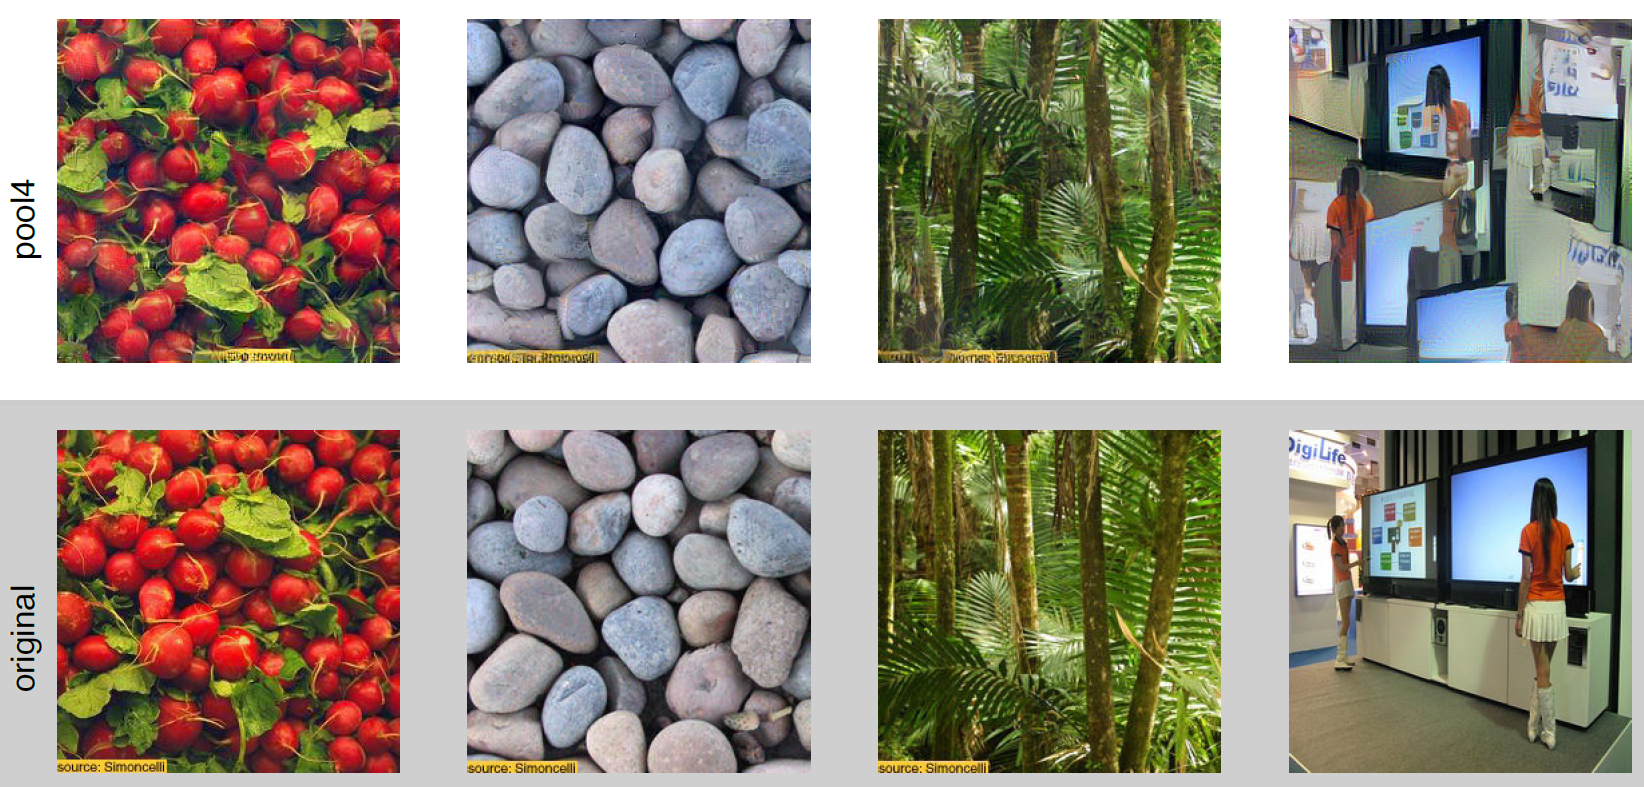
\includegraphics[width=0.8\linewidth]{./img/textures.png}
	\end{center}
	\caption{Ejemplos de sintesis de texturas utilizando Redes Neuronales Convolucionales}
	\label{fig:textures}
      \end{figure}
    
      Transferir el estilo de una imagen a otra puede ser considerado un problema de transferencia de texturas. 
      En la transferencia de texturas el objetivo es sintetizar la textura de la imagen de muestra de forma restringida.
      Estas restricciones permiten preservar el contenido semantico de la imagen a la cual se le desea transferir la textura.
      Teniendo en cuenta todo esto, Gatys et al. adapta su idea propuesta para sintetizar texturas a la Transferencia de Estilos.
      Dicho problema, normalmente se encaraba en una rama de la visión de computadoras llamada representación no fotorrealista \cite{Kyprianidis:ArtisticStylization}.
      
      Existen otros algoritmos que utilizan este enfoque, por ejemplo: 
      Hertzmann \cite{Hertzmann:ImageAnalogies}, el cual utiliza analogias de imagenes para transferir la textura de una imagen de estilo a otra imagen. 
      Ashkimin \cite{Ashikhmin:FastTextureTransfer} se centra en la transferencia de la informacion de alta frecuencia de la textura, preservando la informacion a gruesa escala de 
      la imagen de destino. 
      Efros y Freeman \cite{Efros:ImageQuilting} introduce un mapa de correspondencias que incluye las características de la imagen de destino, tales como la intensidad 
      de la imagen para restringir el proceso de sintetizacion de la textura.
      Lee et al. \cite{Lee:DirectionalTextureTransfer} mejora este algoritmo agregando a la tranferencia de textura, informacion adicional acerca de los contornos y bordes.
      
      Aunque estos algoritmos logran resultados notables, todos ellos sufren de la misma limitación fundamental: usan sólo características de bajo nivel de la imagen de destino para
      informar a la transferencia de textura. Sin embargo, un algortimo de transferencia de estilo debe ser capaz de extraer contenido semántico de la imagen de
      destino (por ejemplo, los objetos y el paisaje general). Luego debe informar al procedimiento de transferencia de textura para que represente lo extraido
      junto con el estilo de la imagen de origen. Por lo tanto, un requisito fundamental es encontrar representaciones de la imagen que modelen independientemente las variaciones
      de contenido semántico de la imagen y el estilo que se les presentan. Dicho requisito se puede lograr utilizando los mapas de caracteristicas de las Redes Neuronales Convolucionales \ref{sec:redes_convolucionales}
      entrenadas en el reconocimiento de objetos. Se ha comprobado que estas logran extraer información semantica de alto nivel del contenido de las imagenes \cite{AlexNet}.


    \section{Sintesis} \label{sec:sintesis}
      El algoritmo desarrollado por Gatys et al. es, conceptualmente un algoritmo de tranferencia de texturas que utiliza mapas de caracteristicas de redes neuronales convolucionales. 
      Dado que la modelizacion de la textura se basa en estas mismas representaciones, el metodo de transferencia de estilo se reduce a un problema
      de optimizacion en una unica red neuronal. Las imagenes son generadas minimizando la distancia entre los mapas de caracteristicas de las imagenes de entrada y los mapas de
      caracteristica de la imagen de salida.
      
      Cuando las Redes Neuronales Convolucionales (CNNs) son entrenadas para el reconocimiento de objetos, desarrollan una representación interna de la imagen.
      Dicha representacion composicional, hace que la información del objeto sea cada vez más concreta a lo largo de la jerarquia de las capas de la red. 
      Por lo tanto, a lo largo de las distintas capas de la red, la imagen de entrada se transforma en representaciones que cada vez más se preocupan 
      por el contenido específico de la imagen en lugar del valor de sus píxeles.
      
      Las capas más altas de la red capturan el contenido de alto nivel en términos de objetos y su ordenamiento en la imagen. 
      En cambio, las reconstrucciones de las capas inferiores simplemente pretenden reproducir los valores exactos de píxeles de la imagen original y algunas formas
      basicas como lineas o curvas. 
      Debido a esto, para representar el contenido de una imagen se utilizaran los mapas de características de las capas superiores de la red.
      Para obtener la representacion del estilo de la imagen, se utiliza un espacio de caracteristicas que fue originalmente diseñado para capturar información de texturas.
      Estas representaciones se obtienen calculando la correlacion entre los mapas de caracteristicas de cada capa de la red. 
      
      Incluyendo las correlaciones de multiples capas, se obtiene una representacion que captura información de la textura pero no del ordenamiento global de la imagen.
      Al reconstruir las imágenes a partir de las representaciones obtenidas, se puede observar que producen una version texturizada de la imagen.
      Estas representaciones, que capturan su apariencia general en terminos de colores y estructuras localizadas, seran llamadas representaciones de estilo.
      
      El principal descubrimiento de Gatys et al. es que la representacion del estilo y del contenido de una imagen pueden ser separadas con una Red Neuronal Convolucional entrenada
      para el reconocimiento de objetos. De esta forma, al manipularse independientemente se pueden generar una nueva imagen desde 2 imágenes de entradas distintas, que 
      simultaneamente se corresponda con la representacion del contenido de una imagen y la respresentacion del estilo de la otra.
      
      \begin{figure}[h]
	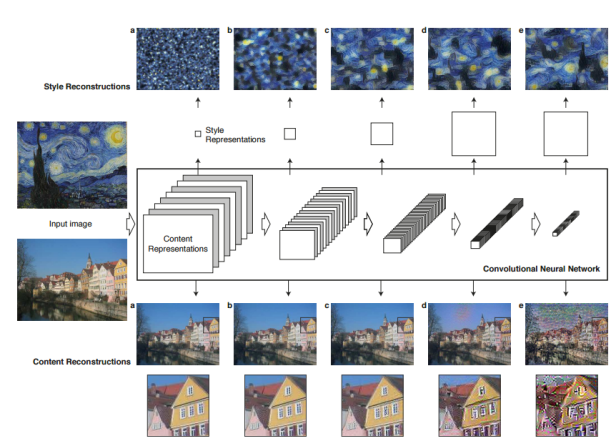
\includegraphics[width=\textwidth]{./img/gatys_1.png}
	\caption{Reconstrucciones del Estilo y Contenido utilizando una CNN}
	\label{fig:gatys_reconstrucciones}
      \end{figure}
	  
      En la figura \ref{fig:gatys_reconstrucciones} se puede observar el resultado de reconstruir el estilo y el contenido utilizando los mapas de caracteristicas que se obtienen al
      realizar una pasada hacia adelante en la red VGG \cite{SimonyanVGG}. Dada una imagen de entrada, en cada capa de la red, ésta se representa como el mapa de caracteristicas en respuesta a los filtros
      que pertenecen a esa capa. Mientras que el número de filtros va aumentando a lo largo de la jerarquía de la red, el tamaño de las representaciones de la imágenes va siendo reducido 
      por algunos mecanismos disminución de resolución(por ejemplo, agrupación) que conduce a una disminución en el número total de unidades por cada capa de la red.
      
      En la parte inferior de la figura \ref{fig:gatys_reconstrucciones} podemos visualizar la información en diferentes etapas de procesamiento en la CNN por la reconstrucción
      de la imagen de entrada solamente conociendo las respuestas de los filtros en una capa en particular. 
      Al reconstruir la imagen de entrada a partir de las capas 'conv1\_1'(a), 'conv2\_1' (b), 'conv3\_1' (c), 'conv4\_1' (d) y 'conv5\_1' (e) de la red VGG,
      se puede observar que la reconstrucción de las capas inferiores es casi perfecta (a,b,c). 
      En cambio, en las capas más altas de la red, información detallada de los píxeles se pierde, mientras que el contenido de alto nivel  de la la imagen se conserva (d,e). 
	
      En la parte superior de la figura \ref{fig:gatys_reconstrucciones} construimos un nuevo espacio de características que captura el estilo de una imagen de entrada.
      La representación de estilo se obtiene calculando las correlaciones entre los mapas de características de diferentes capas de la CNN. Al reconstruir el estilo de la imagen de estilo
      utlizando diferentes subconjuntos de capas de la red ('conv1\_1' (a), "conv1\_1' y 'conv2\_1' (b), 'conv1\_1', 'conv2\_1' y 'conv3\_1' (c),'conv1\_1', 'conv2\_1', 'conv3\_1 ' y 'conv4\_1' (d),
      'conv1\_1', 'conv2\_1', 'conv3\_1', 'conv4\_1' y 'conv5\_1' (e)).
      Esto crea imágenes que coinciden con el estilo de la imagen dada, descartando la información del orden espacial de la escena.
      
      El algoritmo presentado se reduce a un problema de optimización, en el cual se define una funcion de perdida que mide el error entre las representaciones de estilo y contenido 
      de la imagen generada, con las respectivas representaciones de las imagenes de entrada.
      Esta funcion de perdida es una combinación lineal de 2 funciones de perdida distintas, una relacionada al contenido y otra al estilo, las cuales se desarrollan en las secciones \ref{sec:contenido} y \ref{sec:estilo} respectivamente.
      Comenzando desde una imagen de ruido blanco, se va minimizando el valor obtenido por la funcion de perdida, iterativamente, mediante el metodo de descenso por el gradiente, hasta 
      llegar al resultado deseado.
      De esta forma, tanto el estilo como el contenido de la imagen generada se va aproximando al estilo y al contenido de las respectivas imagenes de entrada.
      
      Al ser un algoritmo iterativo, el numero de iteraciones determina el grado de similitud entre la imagen generada con las imagenes elegidas para capturar el contenido y el estilo. 
      La gran influencia de dicho hiperparametro radica en que el mismo determina cuantas veces se minimizara la funcion de perdida mediante el metodo de descenso por el gradiente.
      Ademas, como hemos visto en la seccion \ref{sec:optimizacion}, dicho metodo requiere de otro hiperparámetro llamado tasa de aprendizaje que define el tamaño de cada 
      paso en la iteración.
      Los hiperparámetros requeridos por el metodo de optimización aqui mencionado, son solo algunos de los hiperparámetros exigidos por el algoritmo, en la siguiente seccion se mencionan los demas.
      
    \section{Representacion del Contenido} \label{sec:contenido}
      Generalmente, cada capa de la red define un banco de filtros no lineal cuya complejidad aumenta dependiendo de la jerarquía de la capa en la red.
      Por lo tanto, una imagen de entrada $\overrightarrow{x}$ , se codifica en cada una de las capas de la red convolucional como un mapa de caracteristicas.
      Estos mapas se obtienen a partir de las respuestas de los filtros pertenecientes a dicha capa con respecto a la imagen de entrada.
      Una capa con $N_l$ filtros distintos, tiene $N_l$ mapas de caracteristicas, cada uno de tamaño $M_l$, donde $M_l$ es el ancho por el largo del mapa de caracteristicas.
      Por consiguiente las respuestas de una capa $l$ pueden ser alojadas en una matriz $F^l \in R^{N_l \times M_l}$, donde $F_{i,j}^l$ es la respuesta del $i$-esimo filtro en la posición $j$.
      
      Para visualizar la información codificada en distintas capas de la red, segun su jerarquía, se puede ejecutar descenso por el gradiente a partir de una imagen de ruido blanco
      para encontrar otra imagen que coincida con la respuesta de los filtros de la imagen original. Esto se puede ver en la 
      parte inferior de la figura \ref{fig:gatys_reconstrucciones}.
      Sean $\overrightarrow{p}$ y $\overrightarrow{x}$ la imagen original y la imagen generada, y sean $P^l$ y $F^l$ las respectivas representaciones en la capa $l$.
      La funcion pérdida del contenido se define como el error cuadratico medio entre sus mapas de caracteristicas:
      \begin{equation} \label{eq:perdida_contenido}
       L_{contenido}(\overrightarrow{p},\overrightarrow{x}, l) = \frac{1}{2} \sum_{i,j} (F_{i,j}^l - P_{i,j}^l)^2
      \end{equation}
      El gradiente con respecto a la imagen $\overrightarrow{x}$ puede ser fácilmente calculado utilizando la retropropagación del error, detallada en \ref{sec:backpropagation} (Figura \ref{fig:gatys_generacion} en la parte derecha).
      Por consecuente, se puede ir adaptando la imagen $\overrightarrow{x}$ hasta que genere la misma respuesta que $\overrightarrow{p}$ en una determinada capa de la red.

      
    \section{Representacion del Estilo} \label{sec:estilo}
      Para obtener la representación del estilo de una imagen, se construye un espacio caracteristicas sobre las respuestas de los filtros de cualquier capa de la red. 
      Sobre las respuestas de la CNN en cada capa de la red construimos una representación de estilo que calcula las correlaciones entre las diferentes respuestas de los filtros.
      Estas correlaciones de las caracteristicas estan dadas por la matriz de Gram $G^l \in R^{N_l \times N_l}$, en la cual $G_{i,j}^l$ se calcula como el producto punto entre los vectores
      de los mapas de caracteristicas $i$ y $j$ en la capa $l$:
      \begin{equation}
	G_{i,j}^l = \sum_{k} F_{i,k}^l F_{j,k}^l
      \end{equation}

      Nuevamente, se puede visualizar la informacion capturada por estas caracteristicas construidas, se puede ejecutar descenso por el gradiente a partir de una imagen de ruido blanco
      para encontrar otra imagen que coincida con la representacion de estilo de la imagen original. 
      Esto se hace minimizando la distancia cuadratica media entre las entradas de la matriz de Gram de la imagen
      original y la matriz de Gram de la imagen a generar.
      En la parte superior de la figura \ref{fig:gatys_reconstrucciones} se puede observar la reconstruccion de estilo.
      
      Sean $\overrightarrow{a}$ y $\overrightarrow{x}$ la imagen original y la imagen generada, y sean $A^l$ y $G^l$
      las respectivas representaciones de estilo en la capa $l$, la contribución de esa capa a la función de perdida total del estilo es:
      \begin{equation}
       E_l = \frac{1}{4 N_l^2 M_l^2} \sum_{i,j} (G_{i,j}^l - A_{i,j}^l)^2
      \end{equation}
      De esta forma, la función de pérdida del estilo total queda definida como una combinación lineal de las funciones de perdida de estilo de cada capa:
      \begin{equation}
       L_{estilo}(\overrightarrow{a},\overrightarrow{x}) = \sum_{l=0}^{L} w_l E_l
      \end{equation}
      donde $w_l$ son los factores de peso que tiene cada capa sobre el resultado final, estos factores son introducidos como hiperparámetros del algoritmo. 
      Los gradientes de $E_l$ con respecto a las activaciones de las capas de la red puede ser fácilmente
      calculados utilizando la tecnica retropropagación del error, explicada en la seccion \ref{sec:backpropagation}, (Figura \ref{fig:gatys_generacion} en la parte izquierda).
      
    \section{Transferencia de estilo}
      Para transferir el estilo de una obra de arte $\overrightarrow{a}$ a una fotografia $\overrightarrow{p}$, se genera una nueva imagen
      la cual simultaneamente deba coincidir con la representación de contenido de $\overrightarrow{p}$ y la representación de estilo de $\overrightarrow{a}$ (Figura \ref{fig:gatys_generacion}). 
      Es decir, se minimizan en conjunto la distancia del mapa de caracteristicas de una imagen de ruido con la representacion del contenido de la fotografia
      en una capa y la representacion del estilo de la obra de arte. Por lo tanto la función de perdida total que se minimiza es:
      \begin{equation}\label{eq:objetivo}
       L_{total}(\overrightarrow{p},\overrightarrow{a},\overrightarrow{x}) = \alpha L_{contenido}(\overrightarrow{p},\overrightarrow{x}) + \beta L_{estilo}(\overrightarrow{a},\overrightarrow{x})
      \end{equation}
      Esta funcion combina linealmente las funciones de perdida del contenido y el estilo, por lo que se conforma por 2 terminos principales, uno correspondiente a la funcion de perdida
      del contenido y otro correspondiente a la funcion de perdida del estilo, donde $\alpha$ y $\beta$ son los factores de peso para el contenido y el estilo respectivamente,
      a la hora de combinarlos, los cuales se consideran hiperparámetros. 
      
      \begin{figure}[h]
	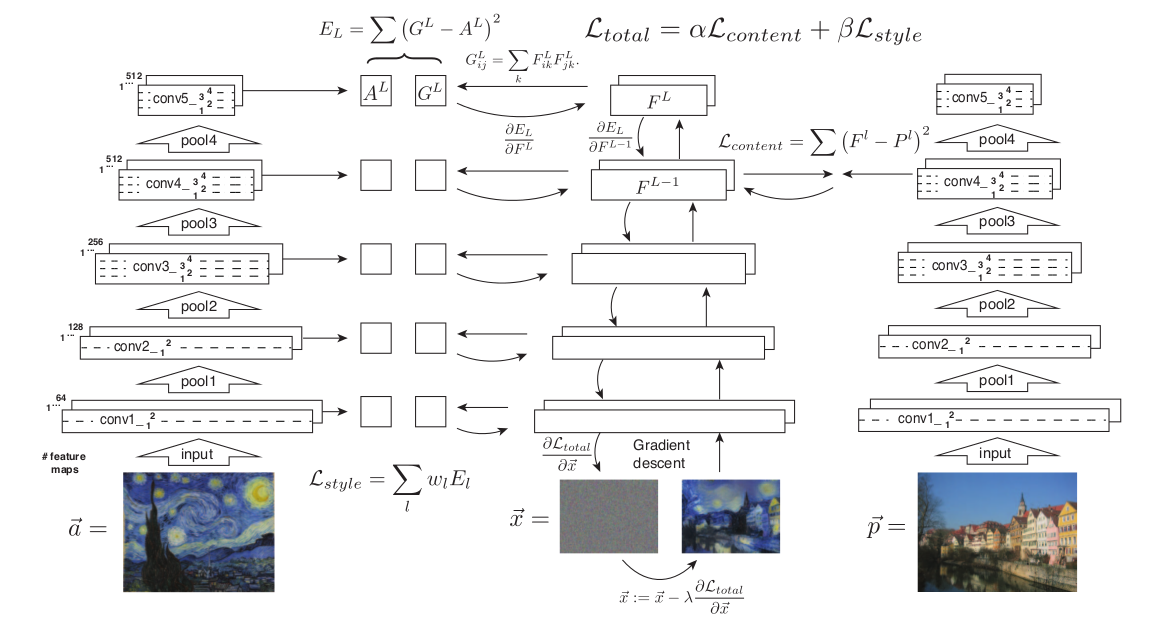
\includegraphics[width=\textwidth]{./img/gatys_method.png}
	\caption{Algoritmo de transferencia de estilo}
	\label{fig:gatys_generacion}
      \end{figure}
      A continuacion se realiza una explicacion detallada de lo que se muestra en la figura \ref{fig:gatys_generacion}:
      
      En primer lugar, las características de contenido y estilo se extraen y almacenan. La imagen de estilo $\overrightarrow{a}$ se pasa a través de la red
      y sus representaciones de estilo $A^l$ en todas las capas incluidas, son calculadas y almacenadas (a la izquierda). La imagen de contenido $\overrightarrow{p}$ pasa a través
      de la red y la representación del contenido $P^l$ en una capa se almacena (a la derecha). Luego a partir de una imagen de ruido blanco $\overrightarrow{x}$ pasa a través de la red y sus
      características de estilo de $G^l$ y sus características de contenido $F^l$ son calculadas.
      
      En cada capa incluida en la representación de estilo, se calcula la diferencia cuadratica media punto a punto entre $G^l$ y $A^l$ para obtener la funcion de perdida del estilo
      $L_{estilo}$ (a la izquierda). Tambien se calcula la diferencia cuadratica media entre $F^l$ y $P^l$ para obtener la funcion de perdida del contenido $L_{contenido}$ (a la derecha).
      La función pérdida total $L_{total}$ es entonces una combinación lineal entre la función de perdida del contenido y la función de pérdida del estilo.
      La derivada de  $L_{total}$ con respecto a los valores de los píxeles pueden ser calculadas con el metodo  de retropropagación del error (en el medio).
      Este gradiente se utiliza de forma iterativa actualizando la imagen $\overrightarrow{x}$ hasta que simultáneamente coincida con las características de estilo de la imagen
      de estilo $\overrightarrow{a}$ y con las características de contenido de la imagen de contenido $\overrightarrow{p}$ (en la parte inferior central).
      
      Finalmente, la salida del algoritmo, a partir de lo enunciado en la ecuación \eqref{eq:objetivo}, sera el argumento $\overrightarrow{x}$
      que minimice la funcion de perdida total, como se puede observar en la ecuacion \eqref{eq:resultante}. 
      \begin{equation} \label{eq:resultante}
       \overrightarrow{x} = \arg\min_{\overrightarrow{x}} L_{total}(\overrightarrow{p},\overrightarrow{a},\overrightarrow{x})
      \end{equation}
      
      \section{Hiperparámetros del algoritmo} \label{sec:hiperparametros}
	A continuación se enumera la lista de hiperparámetros que requiere el algoritmo para ejecutarse y se discute acerca de su influencia en el mismo:
	\begin{itemize}
	 \item Numero de iteraciones: Determina cuantas veces se ejecuta el metodo de descenso por el gradiente para minimizar la funcion de perdida. 
	  A medida que este numero aumenta, mayores son las chances de obtener un resultado aceptado, como se ilustra en la figura \ref{fig:img_iters}.
	  \begin{figure}[h]
	  \begin{center}
	      \begin{tabular}{ccc}
		\subfloat[100 Iteraciones]{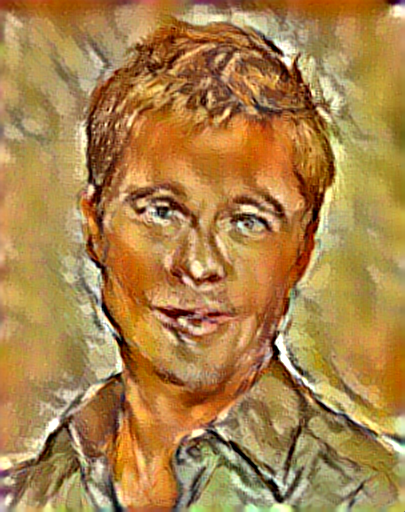
\includegraphics[width=0.2\linewidth]{./img/profile_100.png}}
		& \subfloat[200 Iteraciones]{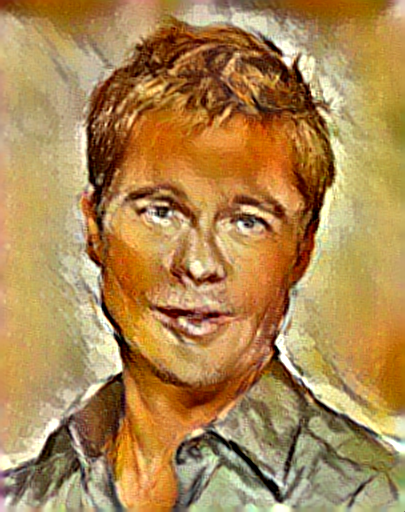
\includegraphics[width=0.2\linewidth]{./img/profile_200.png}}
		& \subfloat[300 Iteraciones]{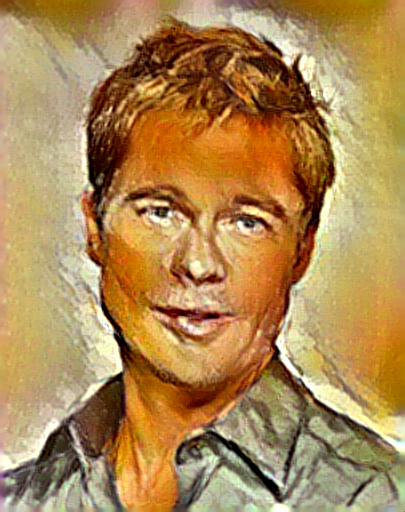
\includegraphics[width=0.2\linewidth]{./img/profile_300.png}}
		\end{tabular}
	    \caption{Ejemplos de obras de arte correspondientes a los estilos seleccionados}
	    \label{fig:img_iters}
	  \end{center}
	\end{figure}
	
	 \item Tasa de aprendizaje: Define el tamaño del paso en cada iteración del descenso por el gradiente. Si esta tasa es muy pequeña, se requieren mayor numero 
	  de iteraciones, sin embargo si es muy grande, se puede caer en un ciclo donde nunca se termine minimizando la funcion de perdida. 
	 \item Red Convolucional: Dependiendo de la red convolucional que se utilice, cambia el tamaño de los mapas de caracteristicas, las capas, etc.
	  Como se menciona en la seccion \ref{sec:cnn_famosas}, existen varias CNNs entrenadas para el reconocimiento de objetos, que tienen arquitecturas
	  muy distintas, al igual que el procesamiento requerido para utilizarlas.
	 \item Capas de la red para la representación de estilo y sus respectivos pesos ($w_l, l \in \{1 \dots L\}$): Como hemos vistos anteriormente en la figura \ref{fig:gatys_reconstrucciones}, 
	 la ubicacion de las capas en la jerarquia de la red, definen distintas experiencias visuales. Como para la representación de estilo se calcula la correlacion entre las capas elegidas,
	 elegir capas intercaladas dentro de toda la jerarquia de la red otorgan una experiencia visual suave y continua.
	 Con respecto a los pesos, por lo general a todas las capas elegidas se les asignada el mismo valor, y a las que no fueron elegidas se les asigna 0.
	 \item Capa de la red para la representacion del contenido: En la figura \ref{fig:content_repr_layers} se analiza la eleccion de la capa $conv2_2$ y la capa $conv4_2$.
	 Al elegir la capa inferior, gran parte de la información detallada de los píxeles en la fotografía y en la imagen generada coincidem (figura \ref{fig:content_repr_layers} al medio).
	 En contraste, al elegir la capa superior, la estructura fina de la imagen se altera, en concordancia con el estilo (figura \ref{fig:content_repr_layers} abajo).
	 \begin{figure}[h]
	    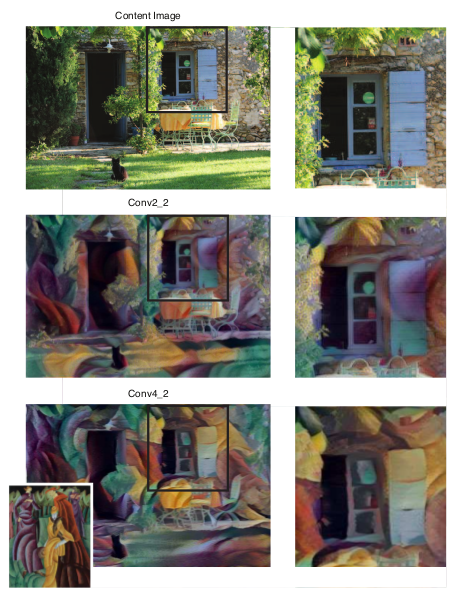
\includegraphics[width=\textwidth]{./img/content_repr_layers.png}
	    \caption{Comparacion de distintas capas de la red para la representación del contenido}
	    \label{fig:content_repr_layers}
	 \end{figure}
	 
	 \item Factores de peso para las funciones de perdida de estilo y contenido en la funcion de perdida total $(\alpha, \beta)$: Esto determina el grado de influencia
	  de cada funcion de perdida. 
	  Un fuerte enfasis sobre el estilo resultara en una imagen que coincida con la apariencia de la obra de arte pero dificilmente se logre observar el contenido de la fotografía 
	  ( $\alpha / \beta = 1 \times 10^{-4}$ figura \ref{fig:ratio_content_style} arriba a la izquierda). Al enfatizar sobre el contenido, se puede visualizar claramente la fotografía,
	  pero el estilo no coincide completamente con la obra de arte ( $\alpha / \beta = 1 \times 10^{-1}$ figura \ref{fig:ratio_content_style} abajo a la derecha).
	  \begin{figure}[h]
	    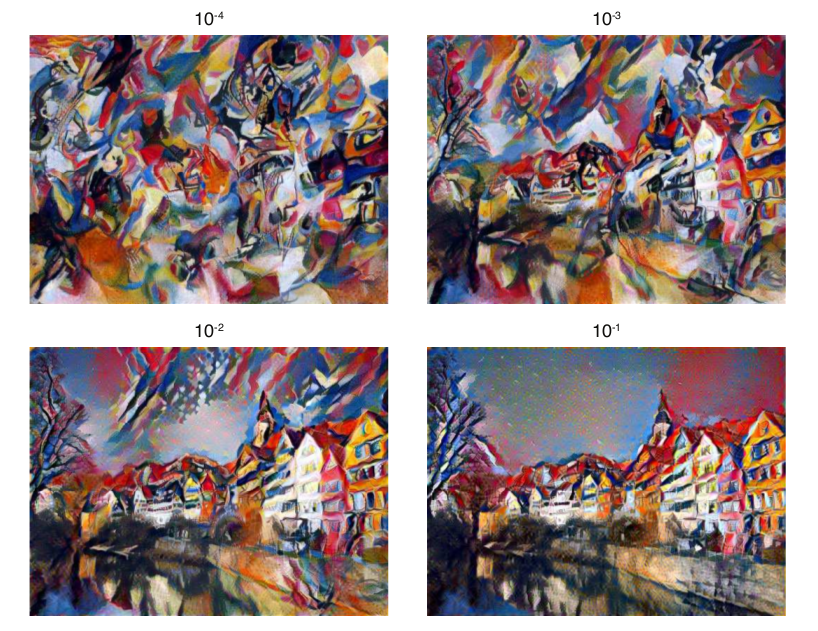
\includegraphics[width=\textwidth]{./img/ratio_content_style.png}
	    \caption{Comparacion de los distintos ratios entre el peso del estilo y el contenido en la funcion de perdida total}
	    \label{fig:ratio_content_style}
	 \end{figure}
	 
	 \item Inicializacion: A pesar de que en las secciones anteriores, en todo momento se comenzo desde una imagen de ruido, el algortimo podria partir desde la imagen
	 de contenido o la de estilo. En las primeras iteraciones se puede observar una inclinacion hacia la imagen de la cual se comienza (comenzar desde ruido o desde la imagen de estilo generan resultado similares) 
	 como muestra la figura \ref{fig:img_init}, pero en el resultado final no termina mostrando una gran influencia.
	  \begin{figure}[h]
	    \begin{center}
		\begin{tabular}{cc}
		  \subfloat[Imagen generada a partir de ruido luego de 100 iteraciones]{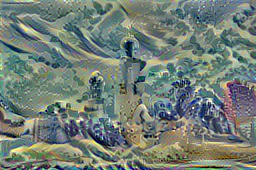
\includegraphics[width=0.4\linewidth]{./img/chicago_wave_100_random.png}}
		  & \subfloat[Imagen generada a partir de la fotografía luego de 100 iteraciones]{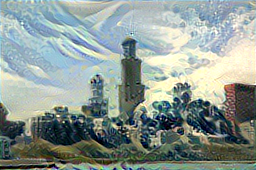
\includegraphics[width=0.4\linewidth]{./img/chicago_wave_100_image.png}}
		  \end{tabular}
	      \caption{Inicializacion del algoritmo}
	      \label{fig:img_init}
	    \end{center}
	  \end{figure}
	
	\end{itemize}

	

\chapter{Elección Automatica de hiperparámetros para Transferencia de estilo}
  \section{Descripción del problema}
    Basado en el algoritmo de transferencia de estilo se pueden obtener resultados muy interesantes, sin embargo, como se menciona en la sección \ref{sec:sintesis}
    es necesario definir el número de iteraciones como un hiperparámetro, que necesita el algoritmo para poder ejecutarse.
    El criterio de elección de este hiperparámetro termina siendo muy influyente en el resultado final. A medida que el número de iteraciones
    aumenta, la función de pérdida del resultado obtenido se va pareciendo cada vez a la función de pérdida calculada a partir de las imagenes de entrada, sin embargo,
    esto influye notablemente en el tiempo de ejecución requerido por el algoritmo.

    \subsection{Evaluación \label{sec:evaluacion}}
      Para poder realizar una comparación entre los distintos resultados generados por el algoritmo, es necesario establecer una métrica, que permita definir si un resultado
      obtenido es mejor que otro, debido a que en lo que respecta a las obras de arte, las evaluaciones suelen ser cualitativas en lugar de cuantitativas.
      Por ello es que se debe buscar una forma de cuantificar estos aspectos cualitativos.

  \section{Solución propuesta \label{sec:solucion}}
    En la solución propuesta en este trabajo se plantea poder definir automáticamente el número de iteraciones que debe ejecutarse el algoritmo hasta lograr obtener un resultado
    aceptable en la minima cantidad de iteraciones posible, reduciendo de esta forma el tiempo de ejecución del algoritmo.
    Con respecto al resto de los hiperparámetros  requeridos por el algoritmo, estos permanecen predefinidos de  antemano.
    La solución consta de 3 módulos principales: un módulo encargado de la generación de la imagen (a partir de una imagen de contenido y otra de estilo), otro módulo encargado de
    evaluar la imagen generada, y un tercer modulo que determina, en base al puntaje de clasificacion obtenido si es necesario continuar el proceso de generacion, como se puede
    observar en la figura \ref{fig:diagrama}.

    \begin{figure}[h]
      \begin{center}
	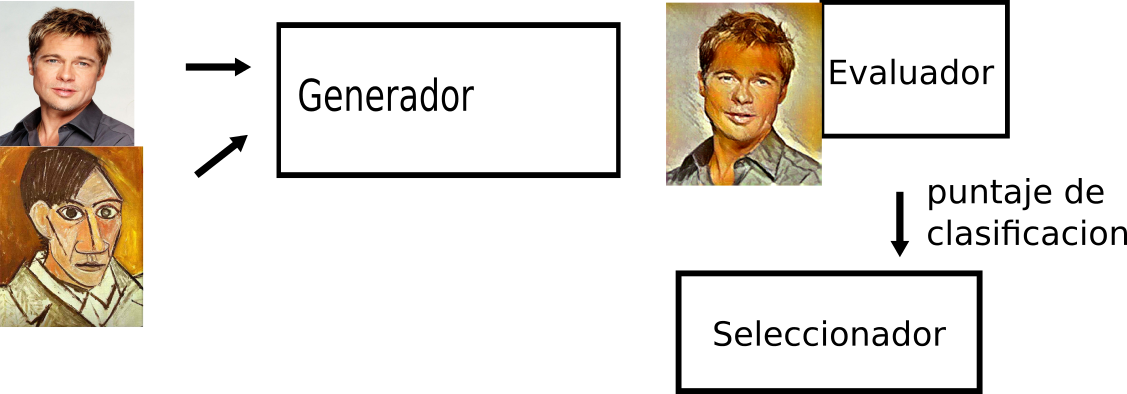
\includegraphics[width=\linewidth]{./img/diagrama.png}
      \end{center}
      \caption{Diagrama de interaccion entre los distintos modulos propuestos}
      \label{fig:diagrama}
    \end{figure}

    \subsection{Módulo de generación de imágenes \label{sec:generador}}
      En este modulo se implementa el algoritmo propuesto por Gatys, para la transferencia de estilo, que requiere como entrada una imagen de estilo,
      una imagen de contenido y como hiperparametro el numero de iteraciones que se ejecutara el optimizador para generar el resultado final.
      La salida de este es una imagen generada donde el contenido se acerca a la imagen de contenido y el estilo se acerca a la imagen de estilo, a medida
      que va aumentando el numero de iteraciones la distancia entre las imagenes de entrada y la imagen generada se va minimizando. Para mas detalles
      acerca del funcionamiento de este modulo, ver figura \ref{fig:gatys_generacion}.

    \subsection{Módulo de evaluación de imágenes: Reconocimiento de estilo \label{sec:evaluador}}
      Como se mencionó en Sec.~\ref{sec:evaluacion}, una de las limitaciones del proceso de transferencia de estilo es que la evaluación de
      la imagen resultante es de carácter cualitativo. A fin de establecer una medida cuantitativa y así controlar el resultado de la generación de
      manera más objetiva, se propone definir un clasificador, que se encargue de reconocer el estilo de una imagen, brindando un puntaje de clasificacion para cada estilo.
      De esta forma la imagen se evalua cuantitativamente segun el puntaje obtenido en el estilo objetivo.
      La entrada de este modulo es la imagen generada y la salida es los puntajes de clasificacion obtenidos por la imagen para cada uno de los estilos.

      A partir de la idea de definir un clasificador de estilos, se realizó una investigación de los posibles metodos para lograr esto. Se decidio basarse en el algortimo presentado en \cite{Karayev:Style_Recognition}.
      Este articulo plantea que los vectores de caracteristicas obtenidos de Redes Neuronales Convolucionales entrenadas para el reconocimiento de objetos, son muy utiles a la hora de
      reconocer estilos, aunque muchos estilos parecieran ser principalmente definidos por las elecciones de colores, los vectores de caracteristicas de las CNN, proveen mucha mas información
      que los vectores obtenidos a partir de histogramas de colores por ejemplo.
      Basado en esta idea, decidimos implementar una version simplificada que consiste en realizar ajuste fino sobre una Red Neuronal Convolucional preentrenda para el reconocimiento de objetos.
      De esta forma se van realizando evaluaciones de la imagen de salida obtenido por el algoritmo generador contra la predicción que realiza el modelo reentrenado para el reconocimiento de estilos.

    \subsection{Módulo de Selección \label{sec:seleccion}}
      Este modulo es el encargado de determinar si es necesario seguir generando imagenes o se acepta la imagen obtenida en la iteracion actual. La entrada de este modulo
      es el vector de puntajes de clasificacion calculados por el modulo generador \ref{sec:generador}, y la salida es un valor binario indicando si se acepta o no la imagen.
      El criterio de selección que se propone para elegir la imagen óptima es el siguiente:
      Basado en la hipotesis de que el resultado generado por el modulo generador \ref{sec:generador} obtenga un puntaje similar que la imagen de estilo en el modulo evaluador
      \ref{sec:evaluador}, se define una tolerancia del $\pm 20\%$ con respecto al puntaje obtenido por la imagen de estilo, en caso de que el resultado obtenga un puntaje que pertenezca
      a este rango, la imagen es aceptada como resultado final, en caso contrario el generador debe seguir iterando hasta obtener un resultado que cumpla con este requisito.


\chapter{Experimentos}
 En este capitulo se exponen los experimentos realizados basados en la solución propuesta en la seccion \ref{sec:solucion}, que permiten validar o rechazar las hipotesis planteadas.
 Para ello se realizaron 2 experimentos principales: El primero consiste en crear un modulo de reconocimiento de estilos artisticos realizando ajuste fino sobre una CNN preentrenada
 para el reconocimiento de objetos. En el segundo experimento se realiza el analisis empirico para la elección del numero de iteraciones mediante el criterio de selección planteado en la
 seccion \ref{sec:seleccion}.

\section{Reconocimiento de estilo}
  Para implementar el modulo de reconocimiento de estilo se decidio realizar ajuste fino sobre una red neuronal convolucional preentrenada para el reconocimiento de objetos.
  A lo largo de esta seccion se detallan las caracteristicas de la implementación de este modulo.
  \subsection{Conjunto de datos}
    El conjunto de datos utilizado para en este trabajo, se construyo a partir del conjunto de datos llamado WikiArt \url{https://www.wikiart.org/}.
    Este conjunto de datos proviene de un proyecto de disponibilidad publica que tiene como objetivo principal hacer accesible el mundo del arte a cualquier persona y en cualquier lugar.
    WikiArt cuenta con una 150.000 obras de arte, de 2.500 artistas. Estas obras se encuentran en museos, universidades y otros edificios civiles de más de 70 países. Aunque la mayoría de estas obras de arte no está en la vista pública.
    Para la implementación de la solución, se utilizo un subconjunto, tomando los 10 estilos que mayor cantidad de obras de arte disponen. A continuacion se enumeran los estilos contemplados:
    \begin{enumerate}
      \item Impresionismo  (14433 obras de arte disponibles)
      \item Realismo (13595 obras de arte disponibles)
      \item Romanticismo (10563 obras de arte disponibles)
      \item Expresionismo (9747 obras de arte disponibles)
      \item Post Impresionismo (7226 obras de arte disponibles)
      \item Surrealismo (6636 obras de arte disponibles)
      \item Modernismo (5969 obras de arte disponibles)
      \item Barroco (5156 obras de arte disponibles)
      \item Simbolismo (4689 obras de arte disponibles)
      \item Neo Clasisimo (3306 obras de arte disponibles)
    \end{enumerate}
      A modo de ejemplo, en la figura \ref{mosaico_estilos} se muestra una imagen correspondiente a cada uno de los estilos elegidos.
	\begin{figure}
	  \begin{center}
	  \def\tabularxcolumn#1{m{#1}}
	  \begin{tabularx}{\textwidth}{@{}cXX@{}}
	  %
	  \begin{tabular}{cc}
	    \subfloat[Modernismo]{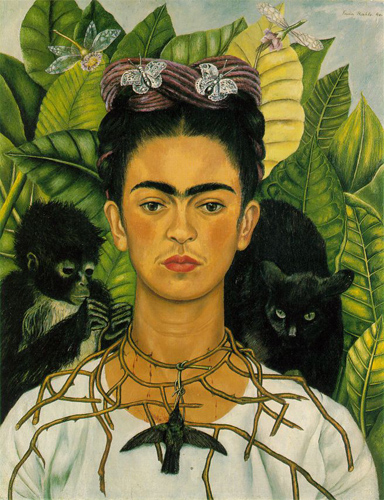
\includegraphics[height=0.15\textheight]{./img/frida_kahlo.jpg}}
	    & \subfloat[Impresionismo]{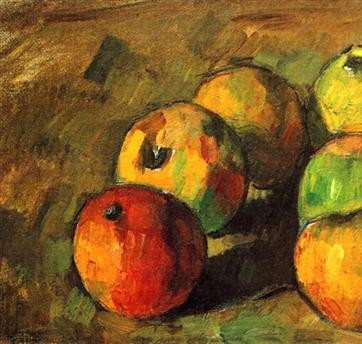
\includegraphics[height=0.15\textheight]{./img/cezanne.jpg}}\\
	    \subfloat[Surrealismo]{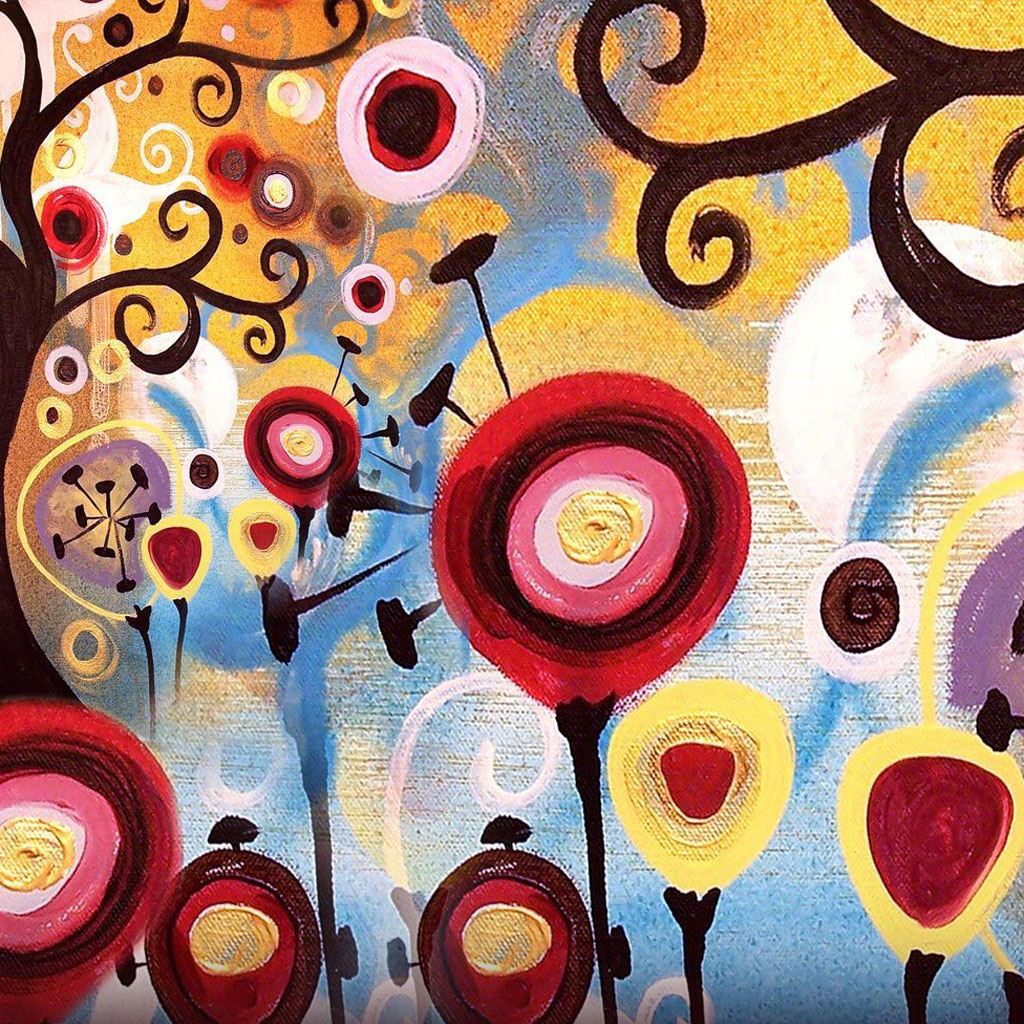
\includegraphics[ height=0.15\textheight]{./img/jhonson_style_candy.jpg}}
	    & \subfloat[Post Impresionismo]{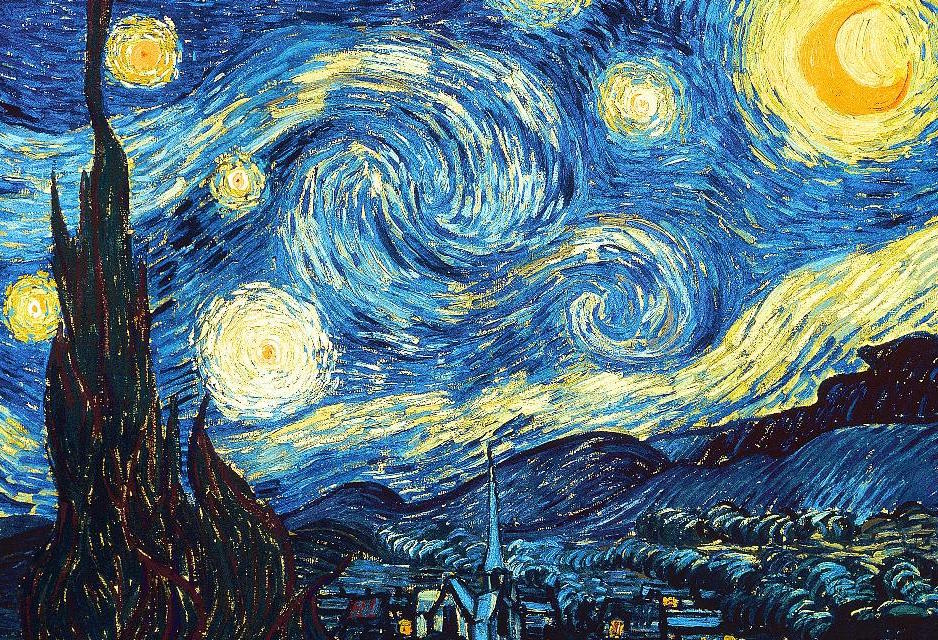
\includegraphics[height=0.15\textheight]{./img/starry_night.jpg}}\\
	    \subfloat[Simbolismo]{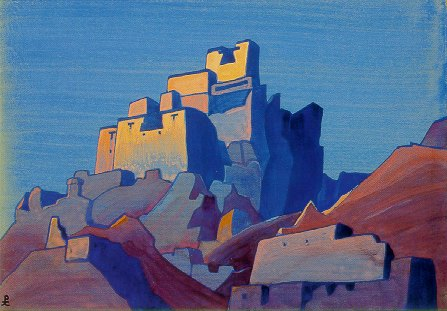
\includegraphics[ height=0.15\textheight]{./img/nicholas-roerich_chiktan-citadel-in-himalayas.jpg}}
	    & \subfloat[Neo Clasisimo]{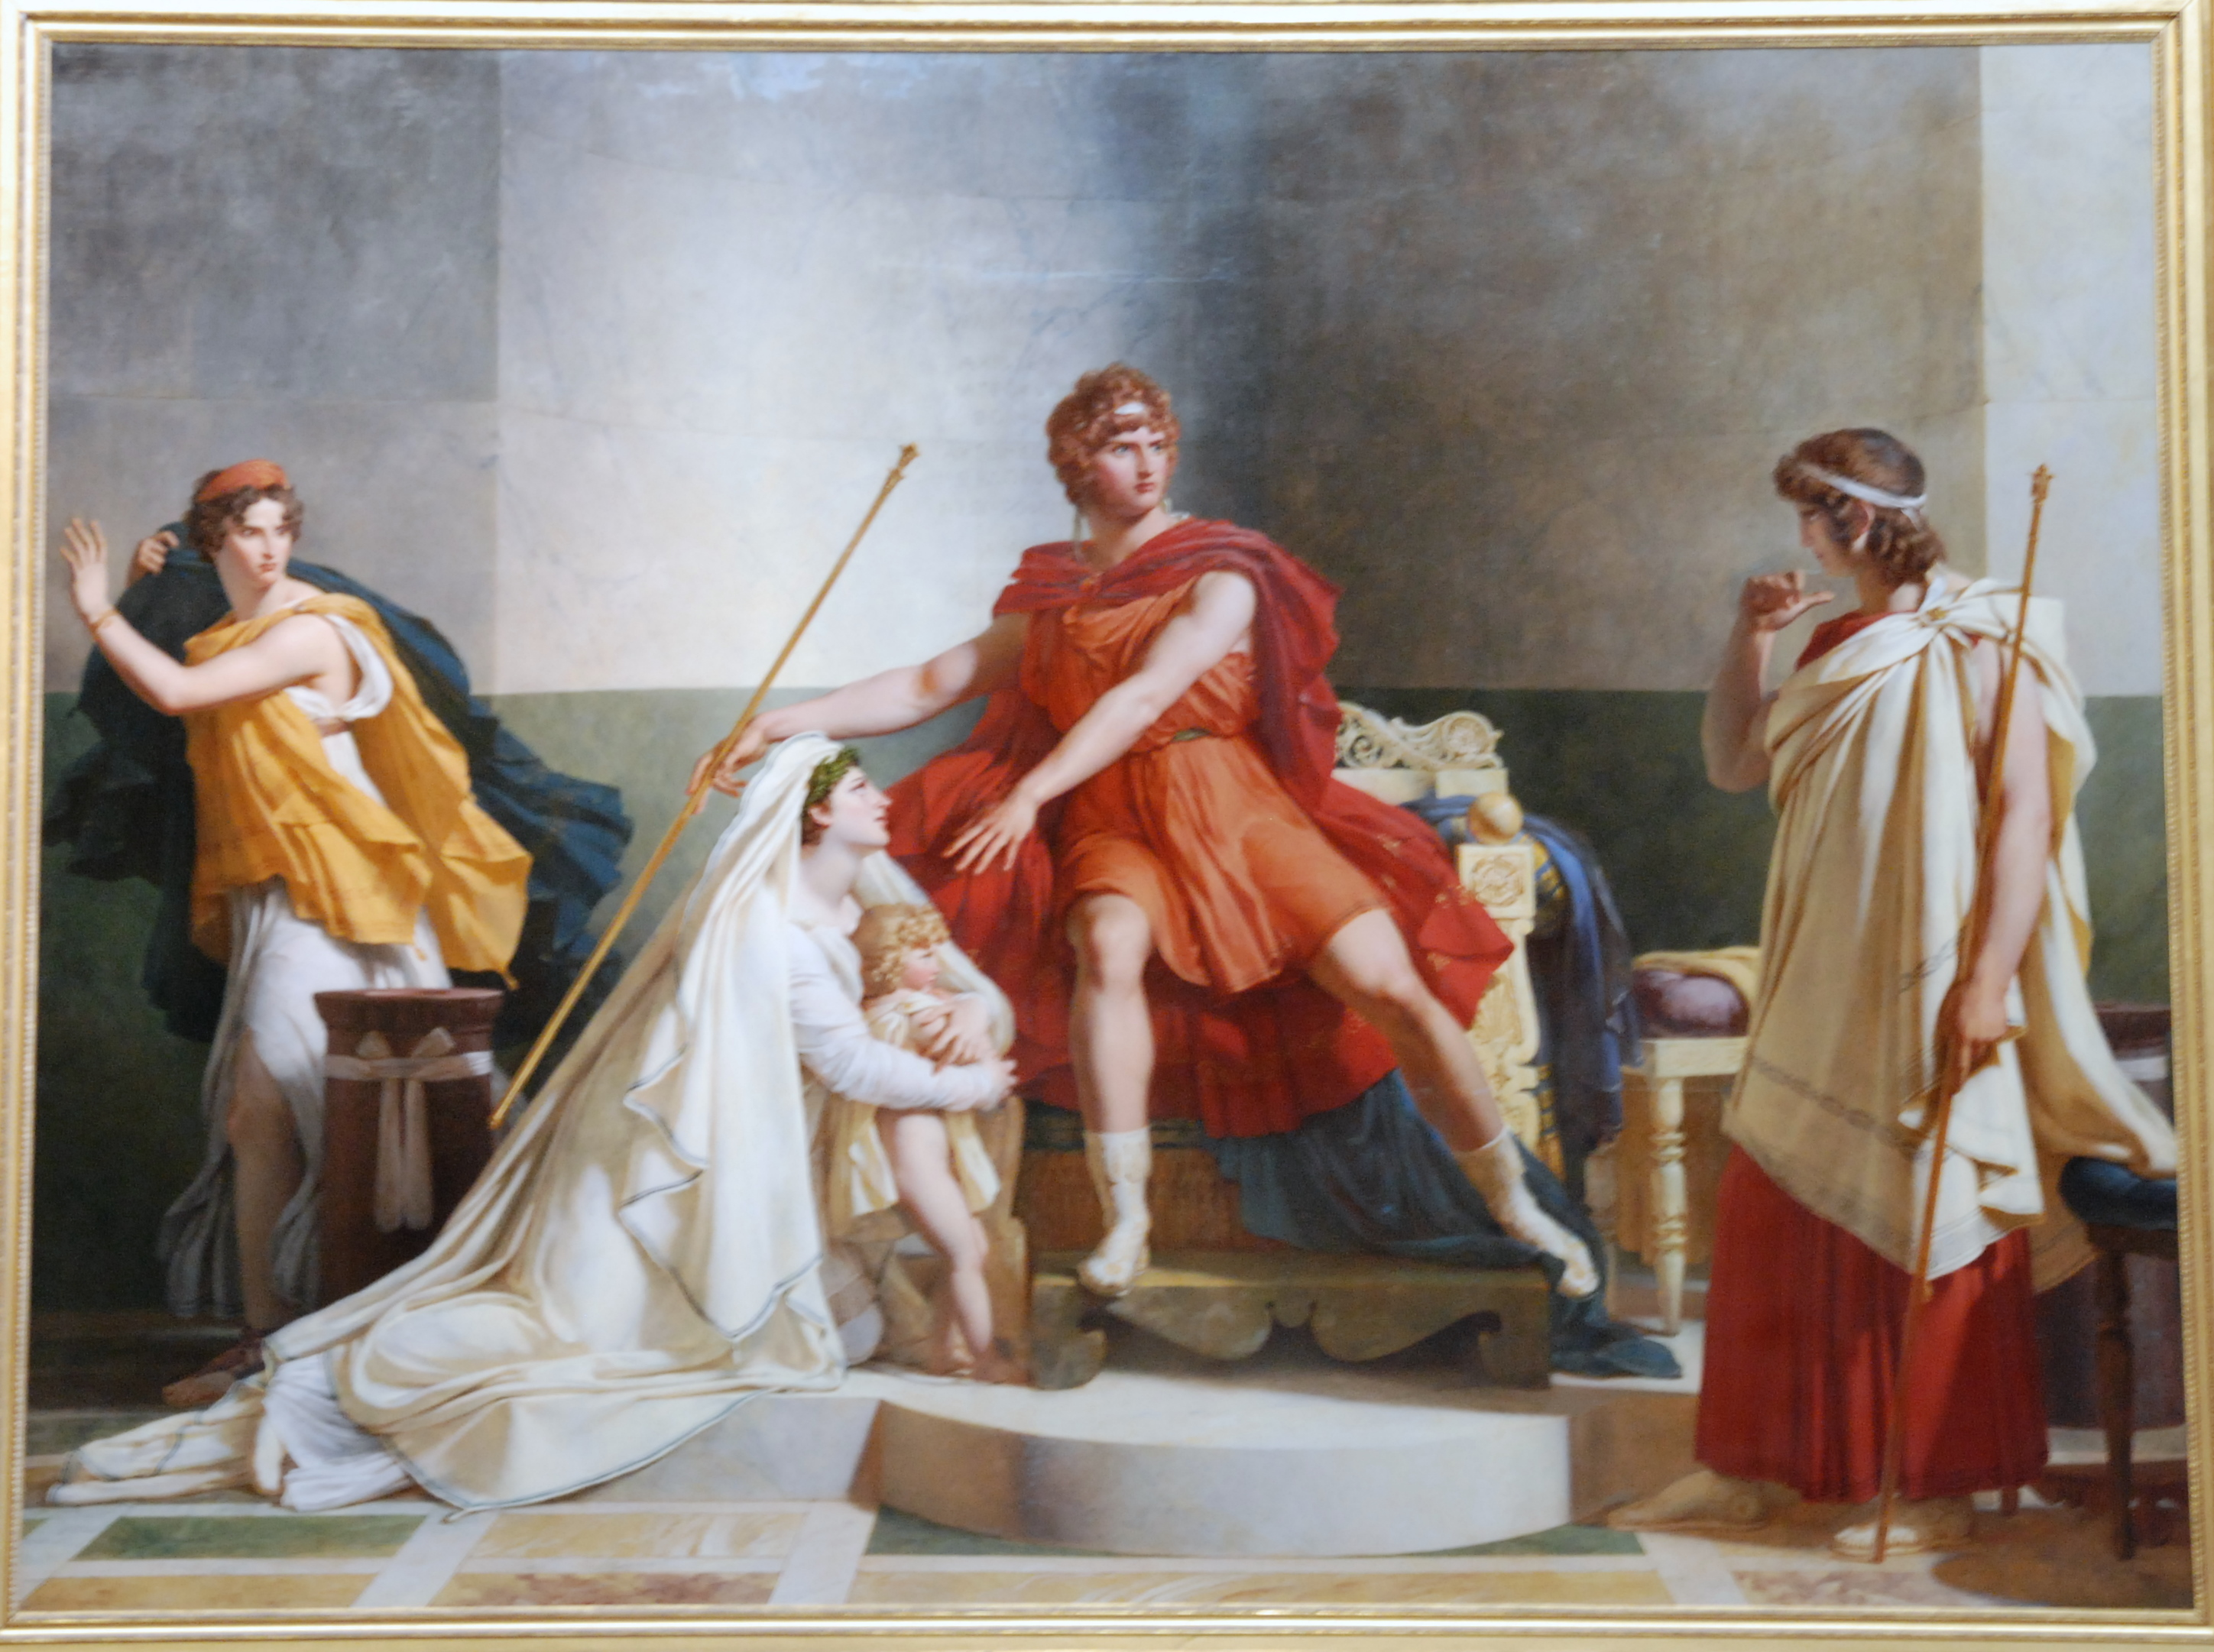
\includegraphics[height=0.15\textheight]{./img/pierre-narcisse-guerin_not-detected.jpg}}\\
	    \subfloat[Romanticismo]{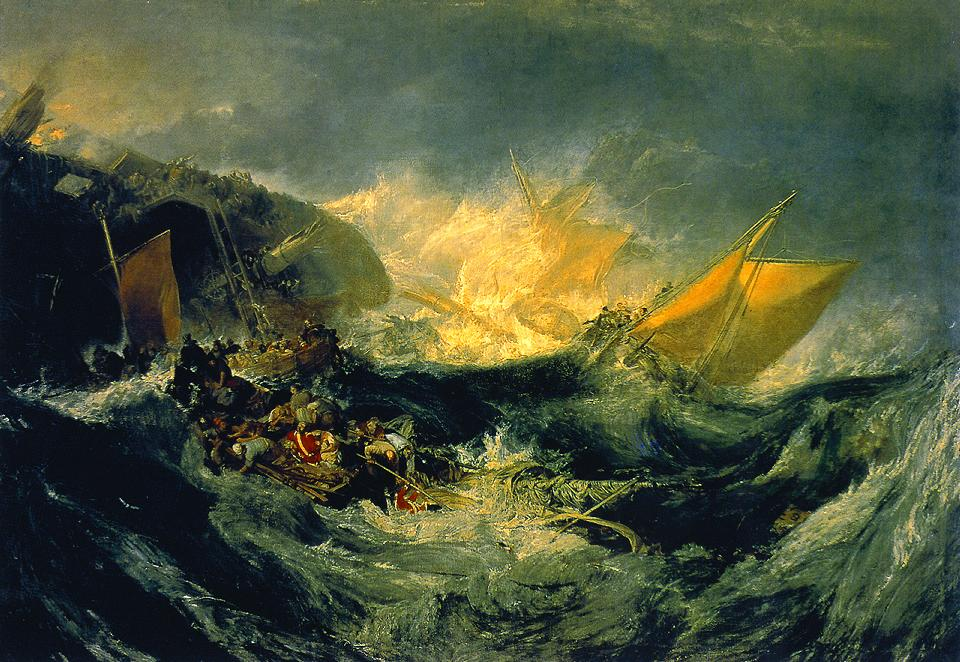
\includegraphics[height=0.15\textheight]{./img/shipwreck.jpg}}
	    & \subfloat[Barroco]{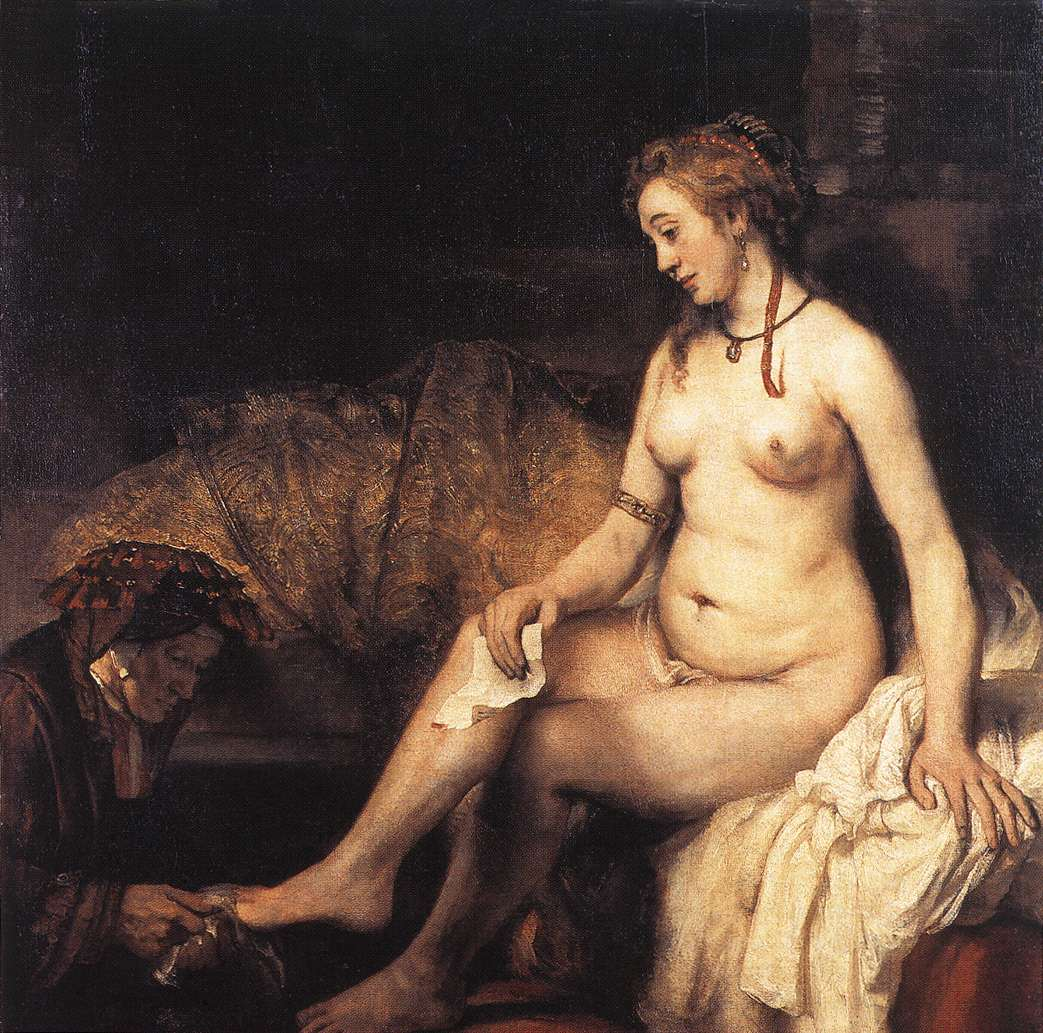
\includegraphics[height=0.15\textheight]{./img/rembrandt_bathsheba-bathing.jpg}}\\
	    \subfloat[Realismo]{\includegraphics[height=0.15\textheight]{./img/vincent-van-gogh_cart-with-red-and-white-ox.jpg}}
	    & \subfloat[Expresionismo]{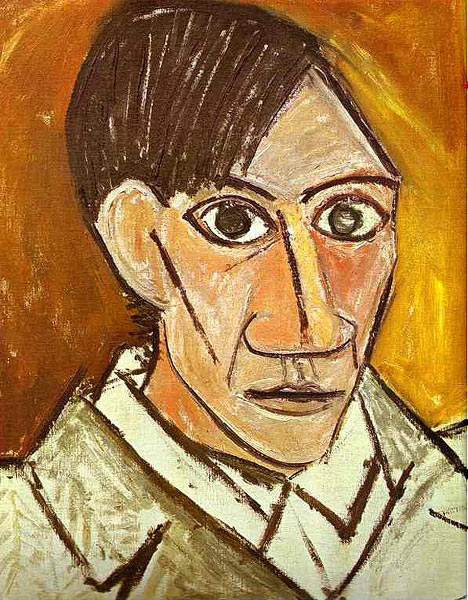
\includegraphics[height=0.15\textheight]{./img/picasso_selfport.jpg}}\\
	  \end{tabular}

	  \end{tabularx}

	  \caption{Ejemplos de obras de arte correspondientes a los estilos seleccionados}\label{mosaico_estilos}
	  \end{center}

	\end{figure}

      \subsubsection{Recolección y construcción del conjunto datos}
	El proceso de recoleccion y construccion de datos consistio en distintas etapas:
	\begin{enumerate}
	 \item Definir los 10 principales estilos de los que se dispongan mayor cantidad de obras, enumeradas anteriormente.
	 \item Descargar cada una de las obras de arte de todos los estilos seleccionados.
	 \item Verificar que la descarga haya sido exitosa y el archivo obtenido este en condiciones para ser utilizado en el proceso.
	 \item Ordenar los archivos segun el estilo al que pertenecen.
	 \end{enumerate}
	Luego de realizado este proceso, el conjunto de datos generado queda conformado por 68807 imagenes.

    \subsection{Detalles de implementación}
      Para realizar el ajuste fino, sobre este conjunto de datos generado, se utilizo la arquitectura de la red AlexNet \cite{AlexNet}, reemplazando la ultima capa por una capa que
      aprenda a reconocer entre los posibles estilos. Los valores con los que se inicializo la red, eran los valores obtenidos al entrenar AlexNet para el reconocimiento de objetos de ImageNet.
      Para reentrenar la red ajustando los valores para el reconocimiento de estilo, se le proveyo el conjunto de datos generado, y se definio realizar 50000 iteraciones para el ajuste fino.
      Para realizar el ajuste fino se utilizó las librerías Caffe y OpenCV en Python, y para el reentrenamiento fue requerido el uso de una GPU GTX 680.

    \subsection{Resultados de clasificación}
    La red obtuvo un 92 \% de precisión en el conjunto de entrenamiento al reconocer estilos.

  \section{Elección del número de iteraciones empleando el módulo de reconocimiento}
    Este experimento consiste en realizar un analisis empirico de la evolucion de los puntajes de clasificacion de estilo a medida que aumenta el numero de iteraciones
    que se ejecuta el modulo de generacion de imagenes.
    \subsection{Conjunto de datos}
      Para ejecutar el procedimiento, es necesario disponer de 2 conjuntos de imagenes, uno correspondiente a las imagenes de contenido y otro correspondiente a las imagenes de estilo.
      Para el conjunto de imagenes de contenido fueron elegidas 5 imagenes, de las cuales 2 son retratos de personas y las 3 restantes son fotografias de paisajes.
      Con respecto al conjunto de imagenes de estilo, para cada uno de los estilos fueron elegidas 3 imagenes aleatoriamente.
    \subsection{Detalles de implementación}
      El proceso consistio en aplicar el algoritmo de transferencia de estilo combinando cada una de las fotos del conjunto de contenido con cada una de las fotos del conjunto de estilo,
      y guardando el resultado cada 10 iteraciones, hasta llegar a las 1000 iteraciones para cada uno de los procesos particulares.
      Ademas para cada combinacion de imagen de estilo e imagen de contenido el algoritmo se ejecuto 2 veces, una comenzando desde la imagen de contenido y otra comenzando desde una imagen de ruido.
      Finalmente todo el conjunto de imagenes obtenido es evaluado por el modulo de reconocimiento de estilo, que otorga un puntaje de la imagen para cada uno de los estilos.
      \subsubsection{Algoritmo de Transferencia de estilo}
	Existen una gran variedad de implementaciónes de código abierto que implementan el algoritmo de transferencia de estilo definido por Gatys.
	La que se decidió utilizar fue la de Justin Jhonson \cite{Johnson:Neural_Style}, la cual posee el mayor grado de aceptación en la industria.
	La principal tecnología utilizada en esta implementación es el Framework Torch, que utiliza como lenguaje de programación a Lua.
	La implementacion  utilizada, permite controlar algunas otras variables mediante hiperparametros extras a lo requerido por el algoritmo originalmente:
	Los principales hiperparámetros adicionales a los requeridos por el algoritmo son:
	\begin{itemize}
	  \item Modelo de Red Neuronal Convolucional preentrenada que se utilizará (existen una variedad de CNN presentadas anteriormente) junto con las capas que se utilizarán de la
	  respectiva red tanto para calcular el estilo como el contenido.
	  \item Imagen desde la cual comenzar la optimización, es posible comenzar desde una imagen de ruido, desde la imagen de contenido.
	  \item Método de optimización a utilizar.
	  \item Tamaño de la imagen generada
	  \item Peso de funciones de perdida de estilo y contenido en la funcion de perdida total \FIXME{esto lo requiere el algoritmo}
	  \item Tasa de aprendizaje para el optimizador
	\end{itemize}


    \subsection{Número de iteraciones vs. Puntaje de clasificación}
      Luego de generar distintas imagenes para cada uno de los estilos, variando entre imagenes de retratos y paisajes como imagenes de contenido, se realizó un analisis
      de la evolucion de los puntajes obtenidos por estas imagenes, a medida que el numero de iteraciones va aumentando. En esta seccion se presentan algunos casos de ejemplo
      que permiten ilustrar lo sucedido en la mayoria de los casos del conjunto de datos generado.
      
      El primer caso presentado en la figura \ref{fig:caso1_tubingen} es el mas simple, como imagen de estilo se utiliza The Shipwreck of the Minotaur, Joseph Mallord William Turner, 1805 (a),
      el cual pertenece al Romanticismo, y como imagen de contenido se utiliza una fotografia de un paisaje de la ciudad de Tubingen, Alemania (b).
      En la imagen (c) se puede observar el resultado obtenido partiendo desde una imagen de ruido, luego de 620 iteraciones y en la imagen (d) se puede observar el resultado partiendo desde
      la imagen de contenido, luego de 600 iteraciones.
      La diferencia entre ambos resultados en este caso es sutil, pero al comenzar desde la imagen de contenido, los bordes y contornos de esta, son mas notorios en el resultado
      que al comenzar desde ruido.
        \begin{figure}[H]
	  \def\tabularxcolumn#1{m{#1}}
	  \begin{tabularx}{\textwidth}{@{}cXX@{}}
	  \begin{tabular}{cc}
	    \subfloat[Imagen de Estilo: Shipwreck, Turner, 1805]{\includegraphics[height=0.2\textheight]{./img/shipwreck.jpg}}
	    & \subfloat[Imagen de Contenido: Fotografia de Tubingen]{\includegraphics[height=0.2\textheight]{./img/tubingen.jpg}}\\
	    \subfloat[Resultado comenzando desde ruido]{\includegraphics[ height=0.2\textheight]{./img/tubingen_shipwreck_620_random.png}}
	    & \subfloat[Resultado comenzando desde el contenido]{\includegraphics[height=0.2\textheight]{./img/tubingen_shipwreck_600_image.png}}\\
	  \end{tabular}
	  \end{tabularx}

	  \caption{Ejemplos de obras de arte correspondientes a los estilos seleccionados}\label{fig:caso1_tubingen}
	\end{figure}
	En cuanto a la evolucion de los puntajes de clasificación, como se puede observar en la figura \ref{fig:puntajes_caso1}, en este caso se cumple con la hipotesis de que el
	estilo predicho para el resultado coincide con el estilo de la imagen de estilo (Romanticismo), al partir desde una imagen de ruido, en las primeras 200 iteraciones el
	clasificador no logra reconocer un claro estilo, pero luego se va normalizando hasta obtener una predicción confiable, ya que la diferencia con los otros estilos es notoria.
	\begin{figure}[H]
	  \begin{center}
	    \subfloat[Evolucion de los puntajes comenzando desde ruido]{\includegraphics[ height=0.35\textheight]{./img/tubingen_shipwreck_random_scores.png}}\\
	    %\subfloat[Evolucion de los puntajes comenzando desde contenido]{\includegraphics[height=0.4\textheight]{./img/tubingen_shipwreck_image_scores.png}}\\
	  \end{center}
	  \caption{Evolucion de los puntajes}
	  \label{fig:puntajes_caso1}
	\end{figure}

	Como segundo caso de analisis se eligio una situacion en la que la prediccion de la imagen resultante coincide con el estilo de la imagen de estilo provista, si se comienza
	el procedimiento desde la imagen de ruido, pero esto no ocurre si se comienza desde la imagen de contenido.
	Para este caso exhibido en la figura \ref{fig:caso2_scream}, como imagen de estilo se utilizo El grito, de Edward Munch, 1893 correspondiente al Expresionismo (a) y como imagen de contenido una fotografia del Golden Gate, un
	icono de la ciudad de San Francisco, Estados Unidos (b). En la imagen (c) se muestra el resultado partiendo desde ruido y en la (d) desde la imagen de contenido, ambas luego de
	540 iteraciones, desde el aspecto visual estos resultados son muy similares, pero para el clasificador son muy distintos como luego de muestra en la figura \ref{fig:puntajes_caso2}.

      	\begin{figure}[H]
	  \def\tabularxcolumn#1{m{#1}}
	  \begin{tabularx}{\textwidth}{@{}cXX@{}}
	  \begin{tabular}{cc}
	    \subfloat[Imagen de Estilo: The Scream]{\includegraphics[height=0.2\textheight]{./img/the_scream.jpg}}
	    & \subfloat[Imagen de Contenido: Fotografia del Golden Gate]{\includegraphics[height=0.2\textheight]{./img/golden_gate.jpg}}\\
	    \subfloat[Resultado comenzando desde ruido]{\includegraphics[ height=0.2\textheight]{./img/golden_gate_the_scream_540_random.png}}
	    & \subfloat[Resultado comenzando desde el contenido]{\includegraphics[height=0.2\textheight]{./img/golden_gate_the_scream_540_image.png}}\\
	  \end{tabular}
	  \end{tabularx}
	  \caption{Ejemplos de obras de arte correspondientes a los estilos seleccionados}\label{fig:caso2_scream}
	\end{figure}

      Al analizar la evolucion de los puntajes predichos por el clasificador nos encontramos con la sorpresa de que el puntaje maximo de clasificación varia dependiendo de la imagen
      en la cual comienza el proceso de tranferencia de estilo, como se puede ver en la figura \ref {fig:puntajes_caso2}, en el grafico (a) se muestra la evolucion de los puntajes
      partiendo de la imagen de ruido, que luego de las 200 iteraciones se termina normalizando al Expresionismo como predicción, lo cual coincide con la imagen de estilo provista.
      Sin embargo, en el grafico (b) se muestra la evolucion de los puntajes de predicción partiendo de la imagen de contenido, en la cual se exhibe al Simbolismo como prediccion
      mayoritaria.

      \begin{figure}[H]
	\begin{center}
	  \subfloat[Evolucion de los puntajes comenzando desde ruido]{\includegraphics[height=0.4\textheight]{./img/golden_gate_thescream_random_scores.png}}\\
	  \subfloat[Evolucion de los puntajes comenzando desde contenido]{\includegraphics[height=0.4\textheight]{./img/golden_gate_thescream_image_scores.png}}\\
	\end{center}
	\caption{Evolucion de los puntajes}
	\label{fig:puntajes_caso2}
      \end{figure}

    \subsection{Validacion de hipotesis para criterio de seleccion}
      Luego se realizar un analisis en varios graficos como los presentados en la seccion anterior se concluyo que la hipotesis sobre que el el puntaje de clasificacion de la imagen
      de estilo y el puntaje de la imagen generada coinciden es falsa, debido a que esto no ocurre en todos los casos analizados, dependiendo de la imagen de contenido el estilo
      que obtiene mayor puntaje de clasificacion puede ser distinto al estilo de la imagen de estilo, ya que la imagen de contenido puede influir en el puntaje de clasificacion de estilo
      de la imagen generada, aunque en mucho menor proporción respecto a la imagen de estilo. Este resultado avala la idea que presenta Gatys acerca de que el estilo y el contenido de una
      imagen no son absolutamente separables.
      
      Debido a esto, el criterio de seleccion que se definio para elegir la imagen optima fue el siguiente: el estilo objetivo, en lugar de ser el estilo correspondiente a la imagen de estilo
      provista para la transferencia de estilo, se definio como el estilo que tiene asignada una mayor
      probabilidad de reconocimiento luego de 1000 iteraciones. Una vez definido el estilo objetivo, se definen los intervalos donde el puntaje obtenido por el estilo objetivo
      supera al puntaje del resto de los estilos. La imagen optima elegida es la correspondiente al numero de iteraciones medio del intervalo donde el estilo objetivo es el maximo. En caso de que haya mas de un de
      un intervalo que cumpla con este requisito, se devuelve una imagen optima de cada intervalo como posibles imagenes optimas para que el usuario elija cual es la optima segun su criterio
      cualitativo.


\chapter{Conclusiones, Perspectivas y trabajos a futuro}
  \section{Conclusiones}
  \section{Trabajos a futuro}
    \FIXME{ \url{https://dailyvisionblog.wordpress.com/2016/07/31/notes-on-texture-networks-feed-forward-synthesis-of-textures-and-stylized-images-and-style-transfer-related-papers/}}
    \subsection{Reconocimiento de Estilos}
      Basandose en la misma idea de entrenar una red convolucional para reconocer solo 10 estilos, se podria extender esto a todos los estilos y utilizando todas las imagenes disponibles
      en WikiArt.
    \subsection{Automatizacion de hiperparámetros}
      Se podría realizar una especie de predefinición del número de iteraciones que requiere cada estilo, ejecutando el algoritmo una gran cantidad de veces y definiendo este valor
      estadisticamente, aunque esto puede llegar a no funciónar correctamente en todos los casos ya que dependiendo de la imagen de contenido, el estilo objetivo podria variar.
    \subsection{Compresion de CNN}
      A partir del articulo presentado por Gatys, se fueron publicando una serie de articulos que presentaban mejoras u optimizaciones al algortimo, ademas de buscar comprimir la red,
      para que una vez entrenada en un dispositivo de gran capacidad de computo, luego pueda ser insertado y ejecutado para transferir estilo en dispositivo menor como lo son los smartphones.
      Por ejemplo se lograron entrenar modelos que transfieran el estilo de una obra de arte en particular, que puede ser ejecutado en un smartphone

\printindex
\bibliography{./tex/biblio}        %use a bibtex bibliography file refs.bib
\bibliographystyle{unsrt}
\end{document}
